%%%%%%%%%%%%%%%%%%%%%%%%%%%%%%%%%%%%%%%%%%%%%%%%%%%%%%%%%%%%%%%%%%%%%%%%
%
% Template latex file for a common article class for class notes
% and write ups. Additional Configuration and styling options are 
% commented out. ex. Table of Contents and Title page
% 
% Author: Amy Bui
% 
%%%%%%%%%%%%%%%%%%%%%%%%%%%%%%%%%%%%%%%%%%%%%%%%%%%%%%%%%%%%%%%%%%%%%%%%
 
\documentclass[12pt]{article}
\usepackage[utf8]{inputenc}
\usepackage{parskip}
\usepackage{tabularx}
\usepackage{array}
\usepackage{appendix}
% \usepackage[showframe=true]{geometry}
\usepackage{changepage}
% \usepackage{csvsimple}
% \usepackage[framemethod=tikz]{mdframed}
% \usepackage[color, leftbars]{changebar}
% \usepackage[inkscapeformat=png]{svg}
% \usepackage{svg}
% \usepackage[inkscape={/Applications/Inkscape.app/Contents/Resources/bin/inkscape -z -C}]{svg}

% Important Configurations
 
%%%%%%%%%%%%%%%%%%%%%%%%%%%%%%%%%%%%%%%%%%%%%%%%%%%%%%%%%%%%%%%%%%%%%%%%
% Reduce margin
%
% \addtolength{\oddsidemargin}{-.85in}
% \addtolength{\evensidemargin}{-.85in}
% \addtolength{\textwidth}{1in}

% \addtolength{\topmargin}{-.85in}
% \addtolength{\textheight}{1in}

% Page format commands:
% Override normal article margins,
% making the margins smaller
\setlength{\textwidth}{6.5in}
\setlength{\textheight}{9in}
\setlength{\oddsidemargin}{0in}
\setlength{\evensidemargin}{0in}
\setlength{\topmargin}{-0.6in}

\setlength{\parindent}{0pt}
%%%%%%%%%%%%%%%%%%%%%%%%%%%%%%%%%%%%%%%%%%%%%%%%%%%%%%%%%%%%%%%%%%%%%%%%


%%%%%%%%%%%%%%%%%%%%%%%%%%%%%%%%%%%%%%%%%%%%%%%%%%%%%%%%%%%%%%%%%%%%%%%%
% Math Symbols
\usepackage{mathtools}
\usepackage{amssymb}
% \usepackage{epsfig}
\usepackage{amsmath,amsthm}
\usepackage{amscd,amsxtra,latexsym}


% add floor and ceiling symbol. Usage: \ceil*{}, \floor*{}
\DeclarePairedDelimiter\ceil{\lceil}{\rceil}
\DeclarePairedDelimiter\floor{\lfloor}{\rfloor}

% multiset \langle ... \rangle
\def\multiset#1#2{\ensuremath{\left(\kern-.3em\left(\genfrac{}{}{0pt}{}{#1}{#2}\right)\kern-.3em\right)}}



%%%%%%%%%%%%%%%%%%%%%%%%%%%%%%%%%%%%%%%%%%%%%%%%%%%%%%%%%%%%%%%%%%%%%%%%

%%%%%%%%%%%%%%%%%%%%%%%%%%%%%%%%%%%%%%%%%%%%%%%%%%%%%%%%%%%%%%%%%%%%%%%%
% Code Sample Styling

% use \lstinline! xxx ! or \begin{lstlisting} ... \end{lstlisting}
\usepackage{listings}

\usepackage{color}
\definecolor{light-gray}{gray}{0.97} % shade of grey
\definecolor{dkgreen}{rgb}{0,0.6,0}
\definecolor{gray}{rgb}{0.5,0.5,0.5}
\definecolor{mauve}{rgb}{0.58,0,0.82}

% \begin{lstlisting}[...] ... \end{lstlisting}
\lstset{frame=none,
    language=Verilog,
    aboveskip=3mm,
    belowskip=3mm,
    stepnumber=0, % set to 0 if you don't like line nums
    showstringspaces=false,
    columns=flexible,
    basicstyle={\small\ttfamily},
    numbers=left,
    numberstyle=\color{black},
    keywordstyle=\color{blue},
    commentstyle=\color{dkgreen},
    stringstyle=\color{mauve},
    backgroundcolor=\color{light-gray},
    breaklines=true,
    breakatwhitespace=false,
    tabsize=2
}

% \newcommand\mylstcaption{}

% \mdfdefinestyle{mymdstyle}{
% hidealllines=true,
% middleextra={
%   \node[anchor=west] at (O|-P)
%     {\lstlistingname~\thelstlisting\  (Cont.):~\mylstcaption};},
% secondextra={
%   \node[anchor=west] at (O|-P)
%     {\lstlistingname~\thelstlisting\  (Cont.):~\mylstcaption};},
% splittopskip=2\baselineskip
% }

% \surroundwithmdframed[style=mymdstyle]{lstlisting}
% \newmdenv[style=mymdstyle]{mdlisting}



%%%%%%%%%%%%%%%%%%%%%%%%%%%%%%%%%%%%%%%%%%%%%%%%%%%%%%%%%%%%%%%%%%%%%%%%

%%%%%%%%%%%%%%%%%%%%%%%%%%%%%%%%%%%%%%%%%%%%%%%%%%%%%%%%%%%%%%%%%%%%%%%%
\usepackage{xcolor}
%% https://tex.stackexchange.com/questions/401750/quick-and-short-command-for-coloring-one-word
\newcommand\shorthandon{\catcode`@=\active \catcode`^=\active \catcode`*=\active }
\newcommand\shorthandoff{\catcode`@=12 \catcode`^=7 \catcode`*=12 }
\shorthandon
\def@#1@{\textcolor{red}{#1}}%
\def^#1^{\textcolor{blue}{#1}}%
\def*#1{\string#1}
\shorthandoff
%% useage: \textcolor{red}{text here}
% \shorthandon
% This is a @test@ of the ^emergency^ bro*@dcast system.
% \shorthandoff
%%%%%%%%%%%%%%%%%%%%%%%%%%%%%%%%%%%%%%%%%%%%%%%%%%%%%%%%%%%%%%%%%%%%%%%%


%%%%%%%%%%%%%%%%%%%%%%%%%%%%%%%%%%%%%%%%%%%%%%%%%%%%%%%%%%%%%%%%%%%%%%%%

%Commands below change page margins (this much space at the titlepage, etc)
\newlength{\toppush}
\setlength{\toppush}{2\headheight}
\addtolength{\toppush}{\headsep}

% Section header Styling
% The commands below change the bold text where it says "Section" into "Question"
% \usepackage{titlesec}
% \titleformat{\section}
% {\normalfont\Large\bfseries}{Question~\thesection:}{1em}{}

% I added this command below to chance "subsections numbers" to be "Question [subsection number]" -AB 1/31/2021
% \titleformat{\subsection}
% {\normalfont\bfseries}{\thesubsection:}{1em}{}

% Page head Styling
% Name and subject of the class
\def\subjnum{EE 156}          % Class Number
\def\subjname{Advance Topics in Computer Architecture}       % Class Name

% Name of the student, university name and which semester
\def\doheading#1#2#3{\vfill\eject\vspace*{-\toppush}%
  \vbox{\hbox to\textwidth{{\bf} \subjnum: \subjname \hfil Amy Bui}%
    \hbox to\textwidth{{\bf} Tufts University, Spring 2023 \hfil#3\strut}%
    \hrule}}

%Command for the title of the document (Homework 0)
\newcommand{\htitle}[1]{\vspace*{1.25ex plus 1ex minus 0ex}%
\begin{center}
    {\large\bf #1}
\end{center}} 
%%%%%%%%%%%%%%%%%%%%%%%%%%%%%%%%%%%%%%%%%%%%%%%%%%%%%%%%%%%%%%%%%%%%%%%%



%%%%%%%%%%%%%%%%%%%%%%%%%%%%%%%%%%%%%%%%%%%%%%%%%%%%%%%%%%%%%%%%%%%%%%%%
% Misc
\usepackage{graphicx} % graphics
\usepackage{enumitem} % listing style (bullet lists)

% below helps with trying to get figures in a row
\usepackage{caption}
\usepackage{subcaption}

% hyperlink styling
% use \href{} and \url{}, and colors table of contents links
% use \href{} and \url{}
% \label{sec:name}
% \hyperref[label]{text}
\usepackage{hyperref}
\hypersetup{
    colorlinks=true,
    linkcolor=blue, % was previously black
    filecolor=magenta,
    urlcolor=blue,
    pdftitle={Template}
}
\urlstyle{same}

% A command for primes (')
\newcommand{\p}%
    {\ensuremath{^{\prime}}}

% a command for double primes ('')
\newcommand{\pp}%
    {\ensuremath{^{\prime \prime}}}

% A command for the Kleene star
\newcommand{\str}%
    {\ensuremath{^{\star}}}

% a command for the double star
\newcommand{\sstr}%
    {\ensuremath{^{\star\star}}}
%%%%%%%%%%%%%%%%%%%%%%%%%%%%%%%%%%%%%%%%%%%%%%%%%%%%%%%%%%%%%%%%%%%%%%%%

% Options for title page, use \maketitle in document
% \author{Amy Bui}
% \title{COMP160 - Algorithms: Class Notes and Practice}


\begin{document}
%% create title page
% \title{(g)ROOT \\ Language Reference Manual}
% \author{Samuel Russo \quad Amy Bui \quad Eliza Encherman \\ Zachary Goldstein \quad Nickolas Gravel}
% \date{\today}
% \maketitle

\doheading{2}{title}{Lab 1}

    %%%%%%%%%%%%%%%%%%%%%%%%%%%%%%%%%%%%%%%%%%%%%%%%%%%%%%%%%%%%%%%%%%%%%%%%
    % Table of Contents
    \setcounter{tocdepth}{2}
    \tableofcontents
    % \pagebreak
    %%%%%%%%%%%%%%%%%%%%%%%%%%%%%%%%%%%%%%%%%%%%%%%%%%%%%%%%%%%%%%%%%%%%%%%%

    \begin{thebibliography}{1}
        \bibitem[1]{sniper}\href{https://snipersim.org/w/The_Sniper_Multi-Core_Simulator}{The Sniper Multi-Core Simulator}
        \bibitem[2]{parallel}O. Tange (2011): \href{https://www.gnu.org/software/parallel/parallel_tutorial.html}{GNU Parallel}  - The Command-Line Power Tool
        \bibitem[3]{splash2}S. C. Woo, M. Ohara, E. Torrie, J. P. Singh and A. Gupta, \href{https://citeseerx.ist.psu.edu/viewdoc/download?doi=10.1.1.48.2356&rep=rep1&type=pdf}{The SPLASH-2 Programs: Characterizaion and Methodological Considerations}, Proceedings 22nd Annual International Symposium on Computer Architecture, Santa Margherita Ligure, Italy, 1995, pp. 24-36
        \bibitem[4]{npb}Bailey DH, Barszcz E, Barton JT, et al. \href{https://www.nas.nasa.gov/software/npb.html}{The Nas Parallel Benchmarks}. The International Journal of Supercomputing Applications. 1991;5(3):63-73. doi:\url{10.1177/109434209100500306}
        \bibitem[5]{book}John L. Hennessy and David A. Patterson. 2017. Computer Architecture, Sixth Edition: A Quantitative Approach (6th. ed.). Morgan Kaufmann Publishers Inc., San Francisco, CA, USA.
        \bibitem[6]{parallelenergy}S. M. Londono and J. P. de Gyvez, "Extending Amdahl's law for energy-efficiency," 2010 International Conference on Energy Aware Computing, Cairo, Egypt, 2010, pp. 1-4, doi: 10.1109/ICEAC.2010.5702300.
        \bibitem[7]{lab0}Bui, Amy. EE156 Lab0 Report. 2023.
    \end{thebibliography}
    \clearpage

    \section{Intro}
        % Notes:
        % \begin{itemize}
        %     \item Study the effects of cache associativity and replacement policy on performance and energy
        % \end{itemize}

        This experiement sweeps different test applications (benchmarks) across different configurations of L3 cache associativity and replacement policy, in order to see effects on power and performance. We analyze the affects of L3 cache associativity and replacement policy on instructions per clock cycle (IPC), energy consumption, and miss rates. It is observed that these sweeps had little effect on energy consumption, and close to none on IPC; variations were seen between the differences in the individual benchmarks when comparing their types of operations. Finally, miss rate appears to decrease with high associativity; however, parallelism does not improve it when the workload is memory intensive.  
        
        % \emph{(Note observations here (i.e. conclusions from Analysis. 1-3 sentences))}

        % It is observed that as L2 cache size increases, total energy consumption of a test application also increases slightly, but the L2 energy consumption increases more noticeably. L2 cache size also affects performance (measured by IPC here) differently depending on how much time a process spends on certain types of instructions; L2 cache size is likely to affect IPC if a benchmark substantially relied on memory access operations. 

    %     The purpose of this experiement is to sweep different test applications (benchmarks) across different configurations of L2 cache sizes, in order to learn the \texttt{SniperSim} tool. We analyze the affects of L2 cache sizes on instructions per clock cycle (IPC) and energy consumption. It is observed that as L2 cache size increases, total energy consumption of a test application also increases slightly, but the L2 energy consumption increases more noticeably. L2 cache size also affects performance (measured by IPC here) differently depending on how much time a process spends on certain types of instructions; L2 cache size is likely to affect IPC if a benchmark substantially relied on memory access operations. 
    % \clearpage

    \section{Experimental Setup}
    \label{sec:setup}
        \begin{table}
        \begin{center} 
            \begin{tabular}{c||c||c}
                \begin{tabular}{|l|}
                    \hline
                    \textbf{Benchmark} \\ 
                    \hline 
                    \hline
                    \texttt{splash2-ocean.cont} \\ 
                    \texttt{splash2-radix}\\
                    \texttt{npb-is}\\
                    \hline 
                \end{tabular}
                & 
                \begin{tabular}{|l|}
                    \hline
                    \textbf{L3 Associativity} \\ 
                    \hline 
                    \hline
                    8 \\ 
                    16 \\
                    32 \\
                    \hline 
                \end{tabular}
                &
                \begin{tabular}{|l|}
                    \hline
                    \textbf{L3 Eviction Policy} \\ 
                    \hline 
                    \hline
                    \texttt{LRU} \\ 
                    \texttt{SRRIP}\\
                    \texttt{Round Robin}\\
                    \hline 
                \end{tabular}
            \end{tabular}
            \caption{Configuration parameters and values swept in the experiment.}
            \label{table:configurations}
        \end{center}
        \end{table}

        Simulations ran for an x86 architecture simulator, Sniper 7.3 \cite{sniper}. Each were configured with 4 cores and the same L1, L2, and L3 cache sizes (64 KB, 128 KB, and 512 KB, respectively, each using 64 byte blocks); remaining relevant configuration values were set in the \texttt{gainestown.cfg}. Input size used for all tests was preset \texttt{large}. Figure \ref{topology} visualizes the topologies for all simulations since cache sizes remained constant. 

        Three different L3 cache associativities, three different L3 replacement policies, and three benchmarks were swept in this experiment, for a total of 27 simulations (see Table \ref{table:configurations}). L3 is the largest and slowest cached memory unit compared to L1 and L2; it is also shared across the four cores, while each core has their own L1 and L2 caches. Therefore, we picked the lowest performing cache level used by the processing unit to sweep because it is likely to have common impact on performance and energy that is observable on all four cores. The different configurations were simulated with two \texttt{splash2} benchmarks (\texttt{ocean.cont} and \texttt{radix} \cite{splash2}) and one NAS parallel benchmark (\texttt{npb}) (\texttt{is} \cite{npb}). The workloads are briefly described as follow:

        \begin{description}
            \item[\textbf{splash2-ocean.cont}]: The \texttt{ocean} suite of test studies large-scale ocean movements based on currents, and uses 4D array grids and a red-black Gauss-Seidel multigrid equation solver. 
            \item[\textbf{splash2-radix}]: The \texttt{radix} suite uses an iterative radix sort algorithm that generates histograms and has each processor permute array index keys, a process that depends on processors communicating in order to determine keys thorough writes.
            \item[\textbf{npb-is}]: The NASA Advanced Supercomputing (NAS) Parallel Benchmarks (NPB) are a set of benchmarks tuned for highly parallel workloads. The \texttt{is} kernal performs a sorting operation that is important as ``particle method'' code (ex. simulations of mechanics (solid, fluid, etc.) as discrete ``particles''), testing both integer computation speed and communication performance. This benchmark excludes floating point arithmetic. 
        \end{description}

        Three varied replacement policies were chosen in order to observe the effects of different replacement models on power and performance. They are as follow:
        \begin{description}
            \item[\textbf{Least Recently Used (LRU)}]: LRU is a recency-based policy that replaces the least recently used block, which involved tracking when blocks are accessed/re-referenced.
            \item[\textbf{Static Re-Reference Interval Prediction (SRRIP)}]: SRRIP is a policy that uses a re-reference prediction value (RRPV) to ``predict'' the how likely a block will be referenced again; this policy uses 2-bit RRPV and is likely to evict recently inserted cache blocks. 
            \item[\textbf{Round Robin}]: Round robin is a queue-based policy that replaces the cache blocks in sequential order, evicting the oldest block in a set in a first-in-first-out (FIFO) manner.
        \end{description}
        

        Simulations had either 8-, 16-, or 32-way L3 set associativity in order to observe how power and performance changed with the number of ways. L1 and L2 caches remained 4- and 8-way set associative, respectively, and both used LRU by default. SniperSim McPAT could not output data for a 64-way set associativity for the given L3 cache size (512 KB) and block size (64 bytes) and so was excluded from the experiment. 

        All the simulations ran concurrently using bash script(s) and GNU \texttt{parallel} shell tool \cite{parallel}, and post processing of the data were handled with python (v2.7) and bash scripts (included separately). Simulations ran on a python virtual environment and in a detached \texttt{tmux} session, due to long duration of the experiments. Sniper provided data processing tools used were: \texttt{gen\_topology.py}, \texttt{cpi-stack.py}, and \texttt{mcpat.py}.
        
        
        \begin{figure}[hbt!] 
            \centering
            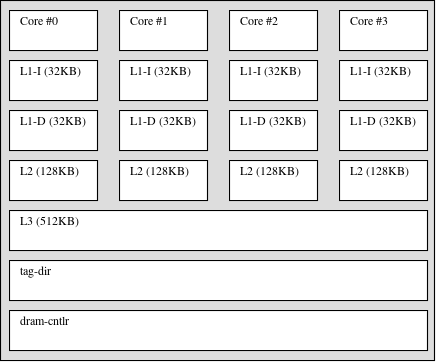
\includegraphics[width=0.5\textwidth]{output/npb-is/8way-lru/topo.png}
            \caption{Topology for \texttt{npb-is}, \texttt{splash2-ocean.cont}, and \texttt{splash2-radix} benchmark tests with all consistent cache sizes: 32 KB L1, 128 KS L2, and 512 KB L3. All benchmarks were run in \texttt{Sniper-7.3} with the \texttt{gainestown} configuration using the \texttt{--viz} and \texttt{--roi} options.}
            \label{topology} 
        \end{figure}
    \clearpage
    %%%%%%%%%%%%%%%%%%%%%%%%%%%%%%%%%%%%%%%%%%%%%%%%%%%%%%%%%%%%%%%%%%%%%%%%

    \section{Results \& Analysis}
        % Notes:
        % \begin{itemize}
        %     \item Measure Hit time and Miss rate (can either be reduces?)
        %     \item Higher associativity reduce miss rate (conflict misses), but increase hit time, and power consumption. (\cite{book}, Ch 2)
        %     \item Overall performance \emph{improvement} over benchmarks?
        %     \item Expect
        % \end{itemize}

    \subsection{Energy Consumption}
    \label{sec:energy}

        Because only associativity and replacement policy were swept across the L3 cache, energy consumption was not expected to significantly vary across an L3 sweep within an individual benchmark. These figures are in the appendix for organization purposes, but are discussed briefly here to expand on differences observed between individual benchmarks. 
        
        Total energy usage across associativity and replacement policies different by hundredths to tenths of joules. The \texttt{npb-is} benchmark had total energy consumption ranging from 16.35 J - 16.87 J, and L3 energy consumption ranging 0.20 J - 0.27 J (Fig. \ref{appfig:power:is:lru} - \ref{appfig:power:is:rr}). The \texttt{splash2-ocean.cont} benchmark had total energy consumption ranging from 61.39 J - 61.91 J, and L3 energy consumption ranging 0.86 J - 1.19 J (Fig. \ref{appfig:power:ocean:lru} - \ref{appfig:power:ocean:rr}). The \texttt{splash2-radix} benchmark had total energy consumption ranging from 1.29 J - 1.31. J, and L3 energy consumption ranging 0.02 J - 0.03 J (Fig. \ref{appfig:power:radix:lru} - \ref{appfig:power:radix:rr}). 
        
        Energy consumption within each benchmark remained consistent, however it is clear that certain workloads used more power than others. As previously observe in \cite{lab0}, \texttt{ocean.cont} consumed about 60x more energy than \texttt{radix}; from their CPI stacks (Fig. \ref{appfig:cpi:ocean:lru} - \ref{appfig:cpi:ocean:rr} and Fig. \ref{appfig:cpi:radix:lru} - \ref{appfig:cpi:radix:rr}, respectively) as well as the workload descriptions in Sec. \ref{sec:setup}, \texttt{ocean.cont} had more memory accesses than \texttt{radix}, which itself was dominated by integer and floating point operations. Fewer memory accesses resulted in less power usage. This, likewise, applies to \texttt{radix} having less power than \texttt{npb-is}, as it also has more memory accessing operations than \texttt{radix} (Fig. \ref{appfig:cpi:is:lru} - \ref{appfig:cpi:is:rr}). \texttt{ocean.cont} is seen to consume 4x more energy than \texttt{npb-is} despite having similar fractions of time spent on memory accessing operations. This is likely due to \texttt{npb-is} being a parallel workload and parallelism can be exploited for energy savings \cite{parallelenergy}. Memory accesses consuming more energy and parallelsim contributing to saving energy is also seen in Fig. \ref{fig:all:L3Peak}, where each L3 peak dynamic power of all three benchmarks are plotted together; \texttt{ocean.cont} peaked higher than the other two. 

        \begin{figure}[htb!]
            \centering
            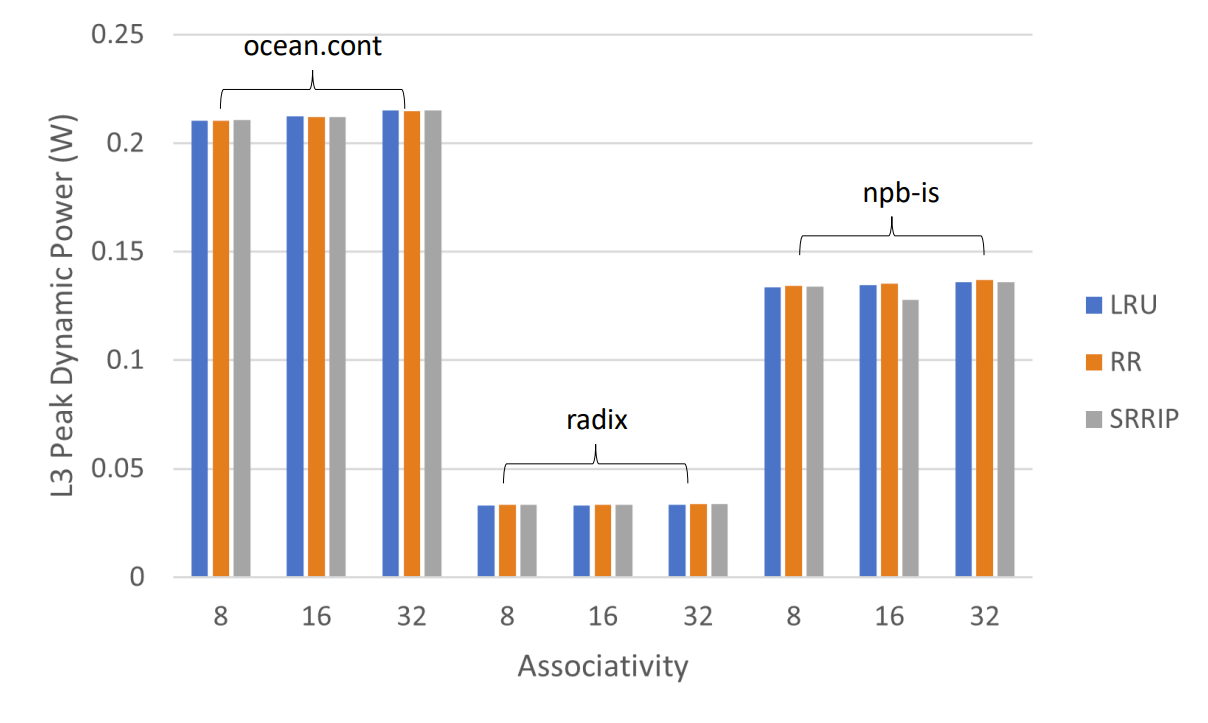
\includegraphics[width=0.8\textwidth]{./allL3PeakDynamicslabeled.png}
            \caption{L3 cache associativity and replacement policy graphed against \textbf{Peak Dynamic Power of L3} for all three benchmarks. }
            \label{fig:all:L3Peak}
        \end{figure}
        % \clearpage

        In plotting the individual \emph{peak} dynamic power across the workloads, we see that in most cases, as associativity increases, so do peak dynamic power of the processor (Fig. \ref{fig:peakDynamicProcessor}) and the L3 cache (Fig. \ref{fig:peakDynamicL3}). While this matches the general observation that higher associativity increases power consumption (\cite{book}, Ch 2), the increases are only on the order of tenths or hundreths (for processor) and thousandths (for L3) of Watts. More significant differences may be observed in tests sweeping higher associativity, block sizes, or more diverse workloads (in terms of fractions of memory accesses). 

        \begin{figure}[htb!]
            \begin{adjustwidth}{-2.75cm}{}\begin{tabular}{ccc}
                \begin{subfigure}{0.42\textwidth}
                    \centering
                    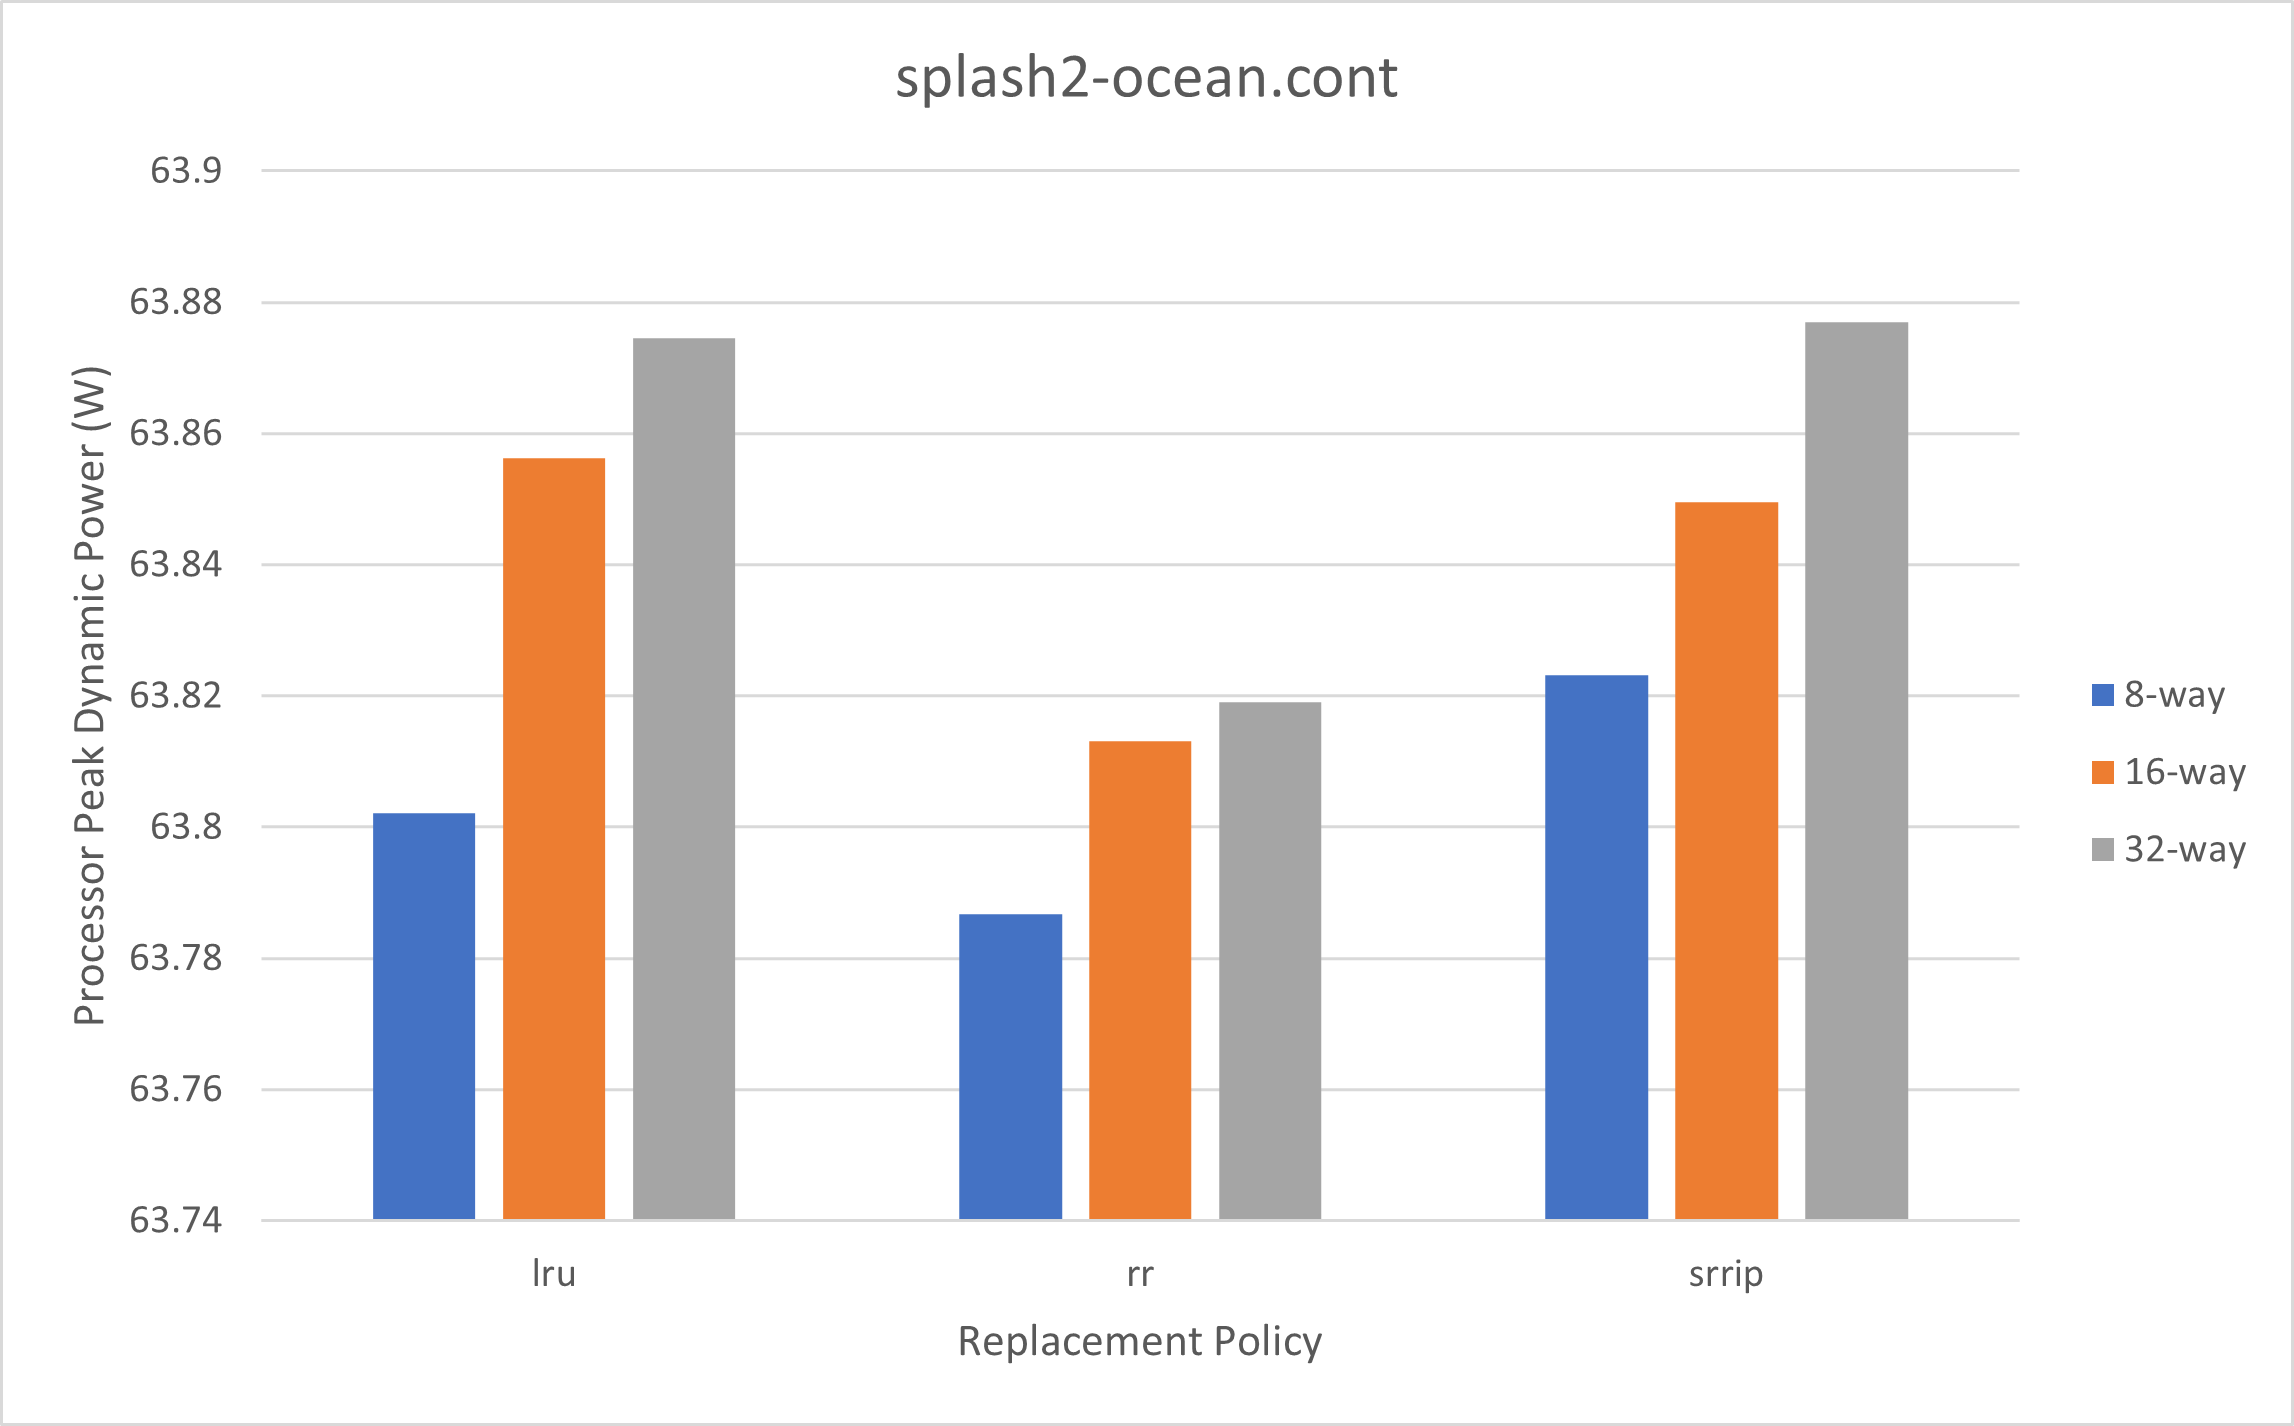
\includegraphics[width=1\textwidth]{./oceanPeakDynamicsProcessor.png}
                    \caption{}
                    \label{ProcPeak:ocean}
                \end{subfigure} &
                \begin{subfigure}{0.42\textwidth}
                    \centering
                    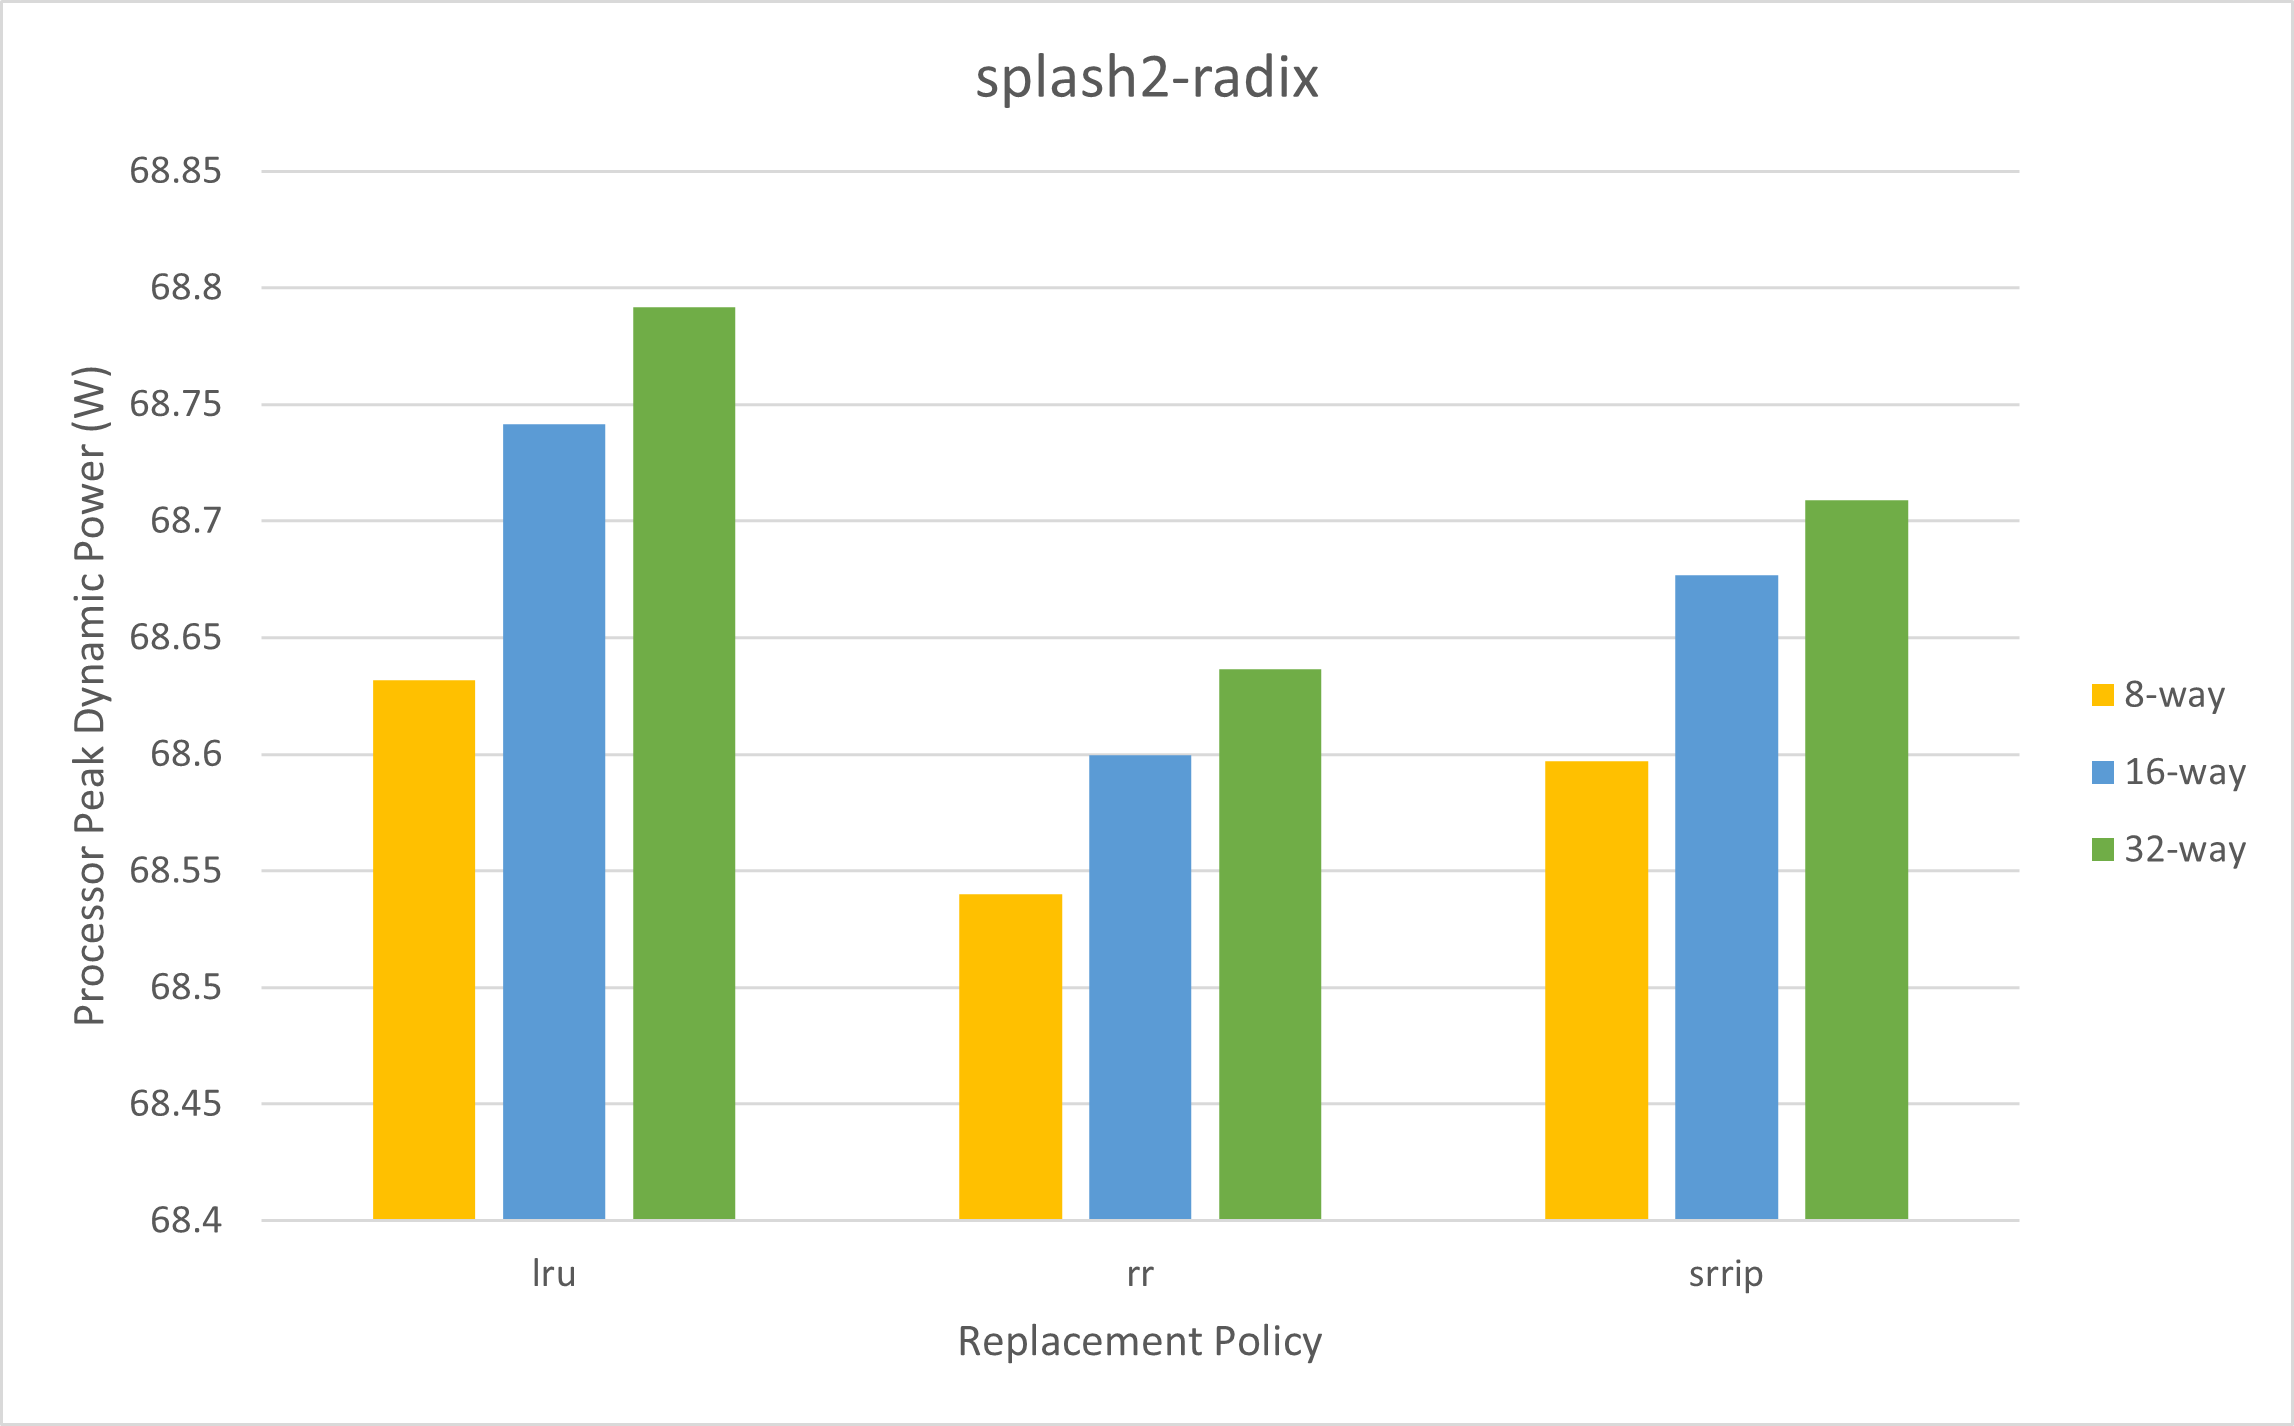
\includegraphics[width=1\textwidth]{./radixPeakDynamicsProcessor.png}
                    \caption{}
                    \label{ProcPeak:radix}
                \end{subfigure} &
                \begin{subfigure}{0.42\textwidth}
                    \centering
                    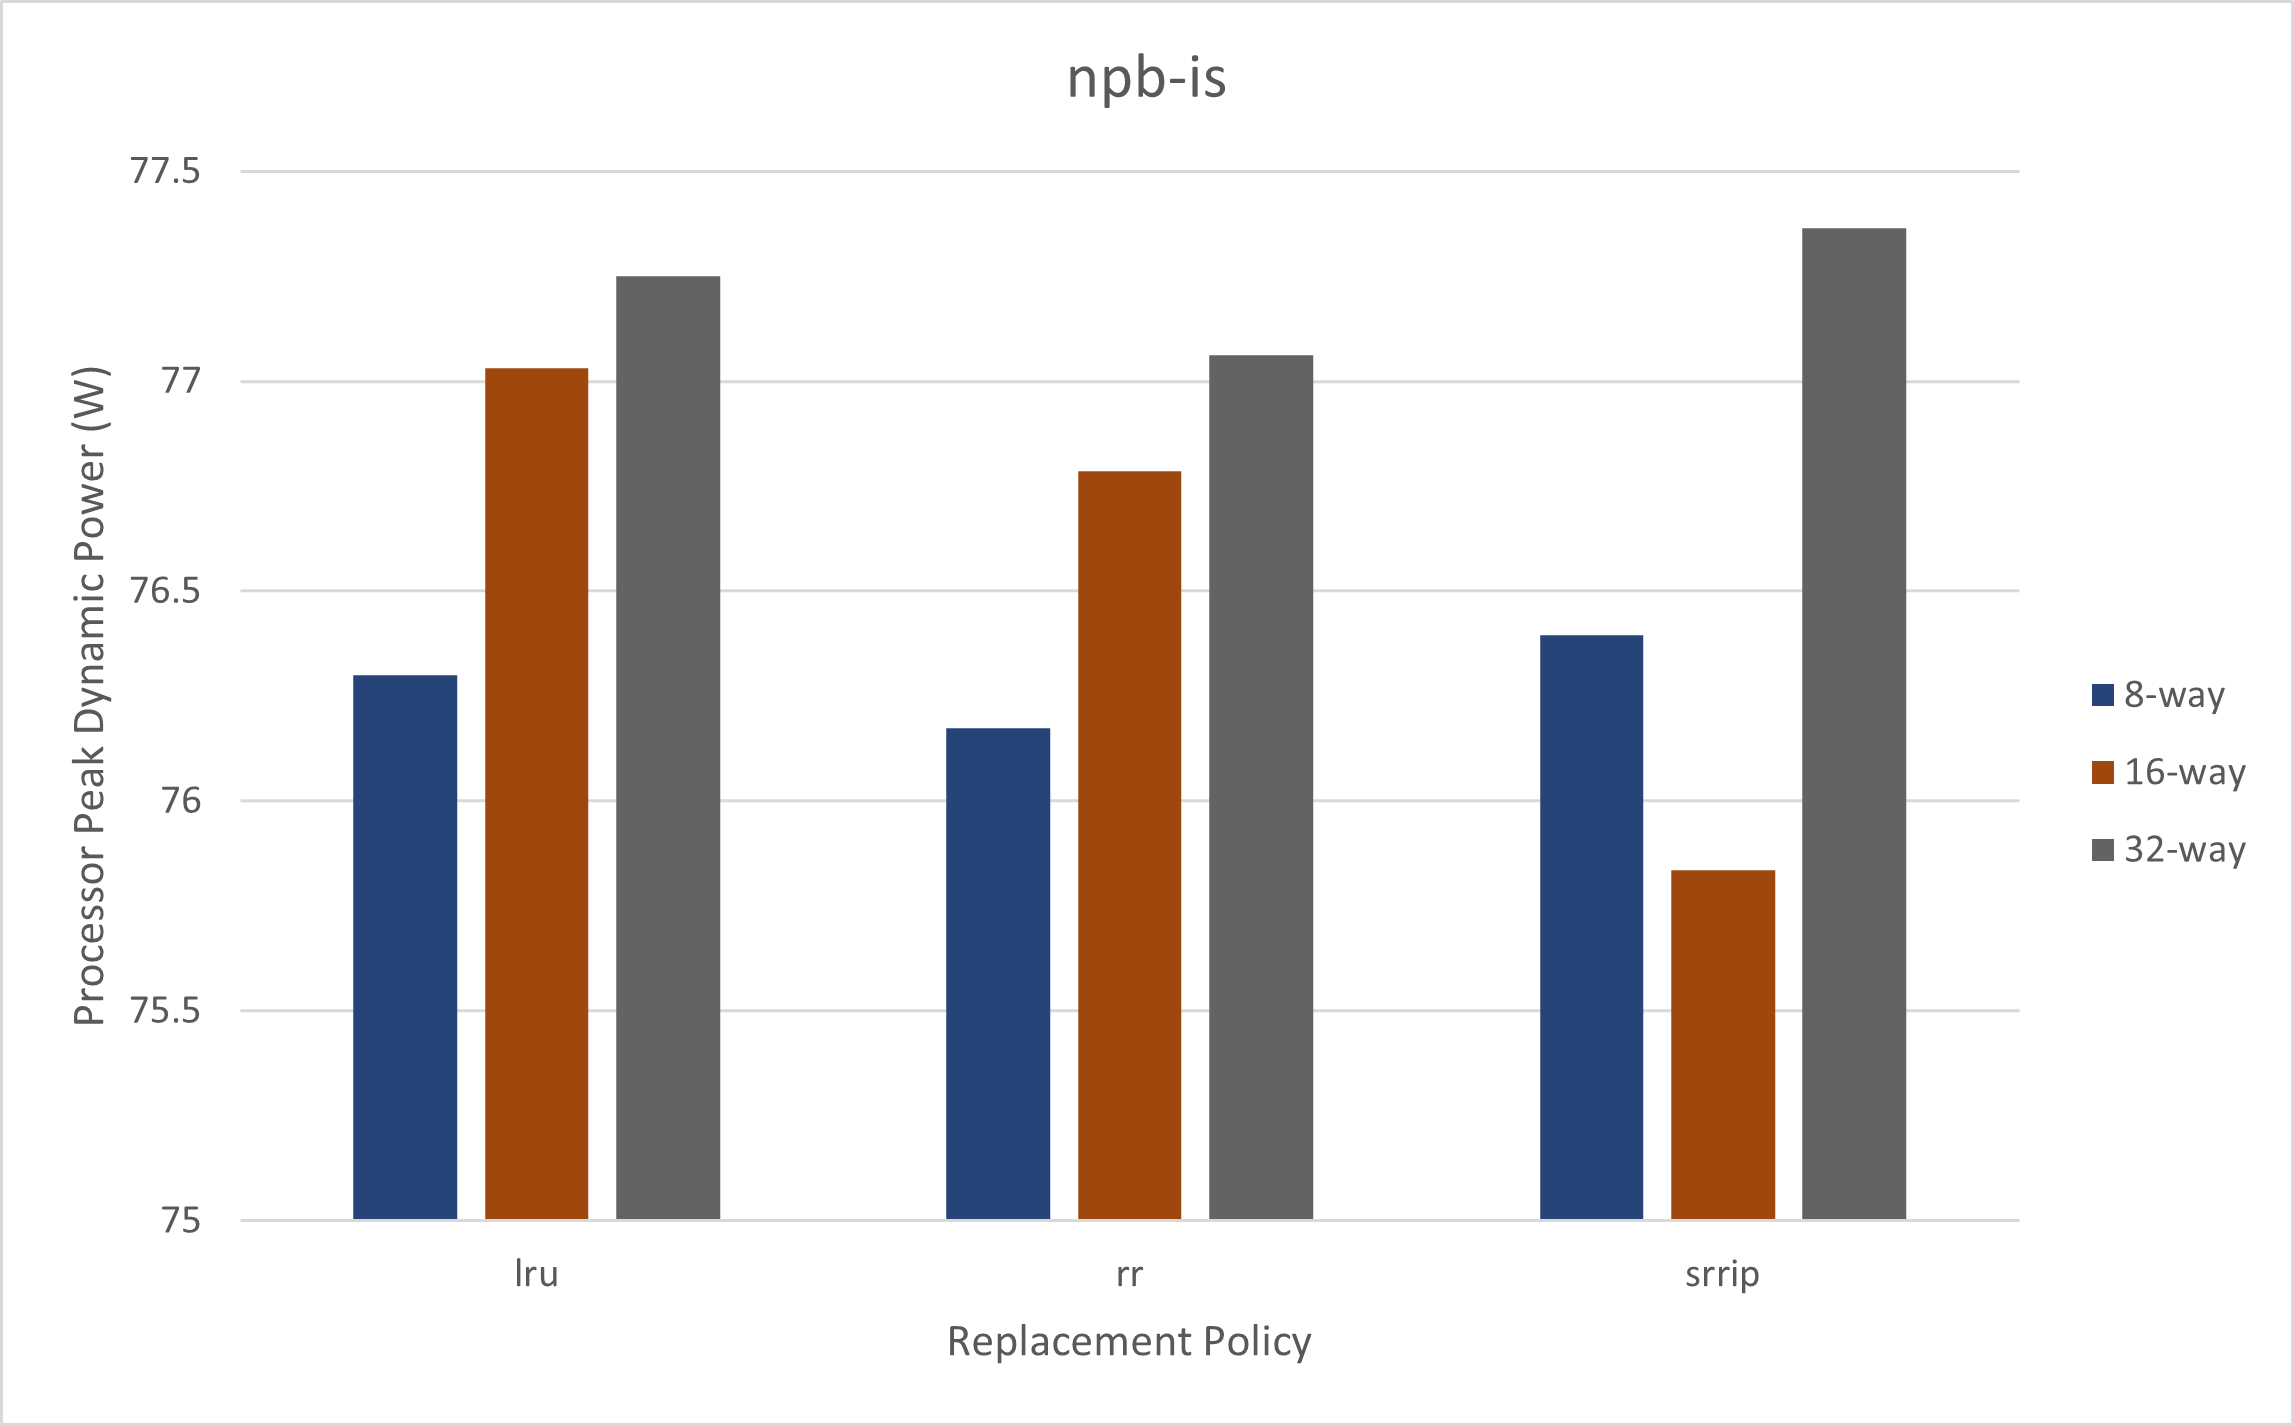
\includegraphics[width=1\textwidth]{./isPeakDynamicsProcessor.png}
                    \caption{}
                    \label{ProcPeak:is}
                \end{subfigure} 
            \end{tabular}\end{adjustwidth}
            \caption{Peak Dynamic Power of Processor across the L3 sweep.}
            \label{fig:peakDynamicProcessor}
        \end{figure}
    
        \begin{figure}[htb!]
            \begin{adjustwidth}{-2.75cm}{}\begin{tabular}{ccc}
                \begin{subfigure}{0.42\textwidth}
                    \centering
                    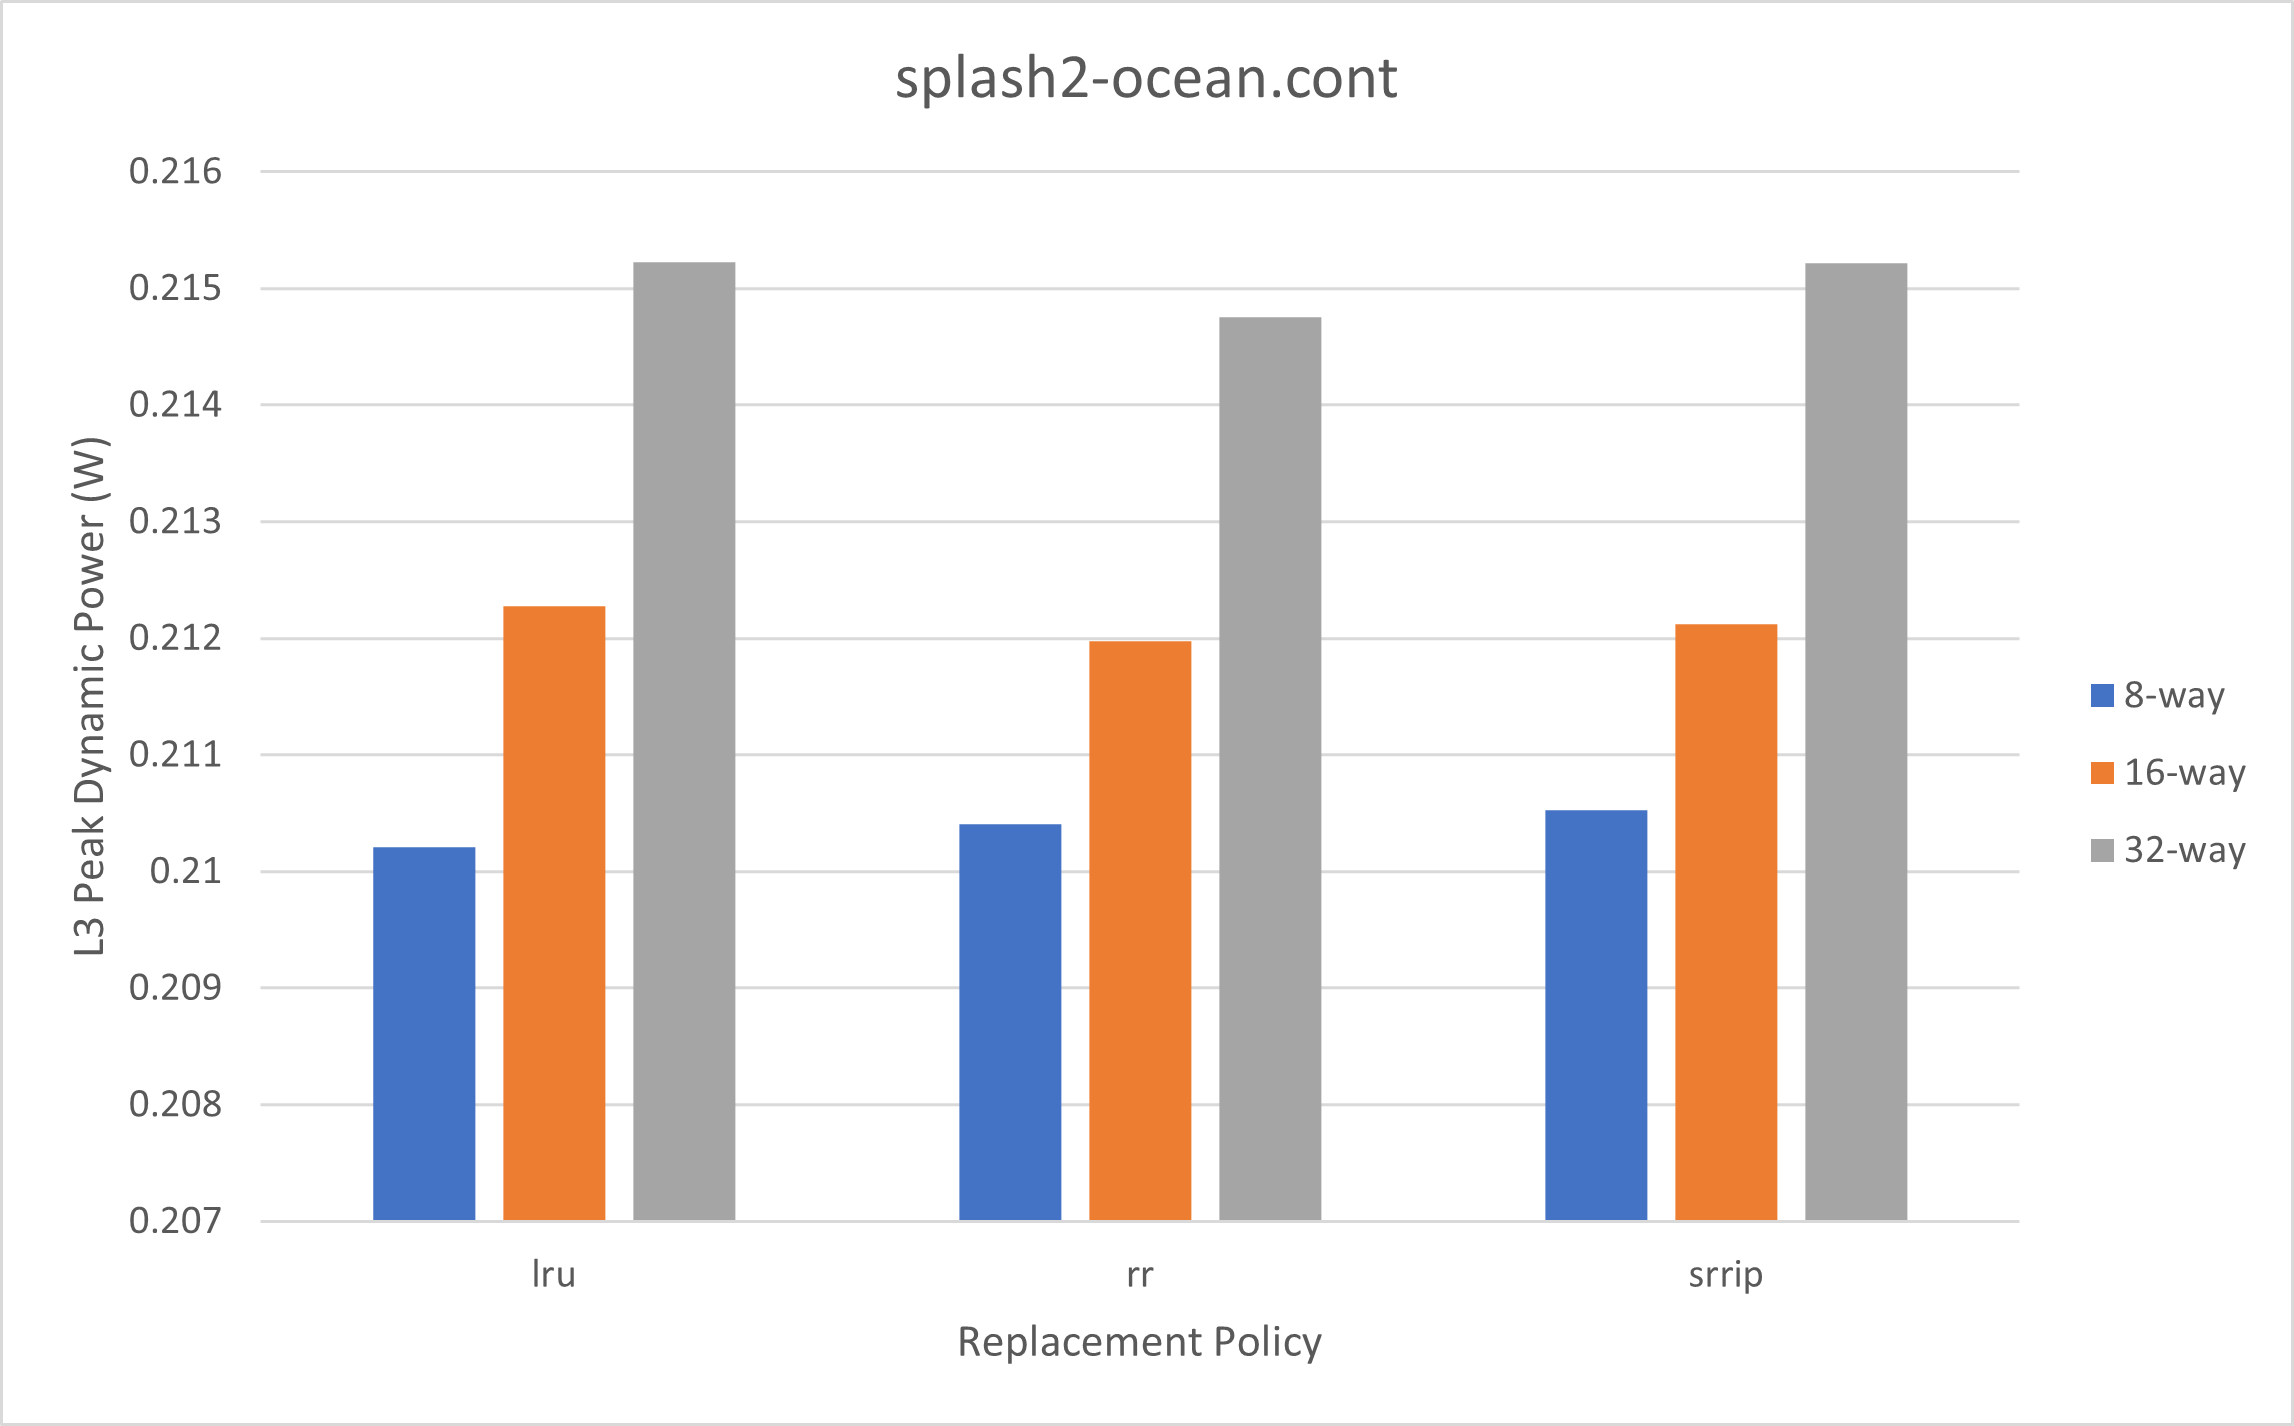
\includegraphics[width=1\textwidth]{./oceanPeakDynamics.png}
                    \caption{}
                    \label{L3Peak:ocean}
                \end{subfigure} &
                \begin{subfigure}{0.42\textwidth}
                    \centering
                    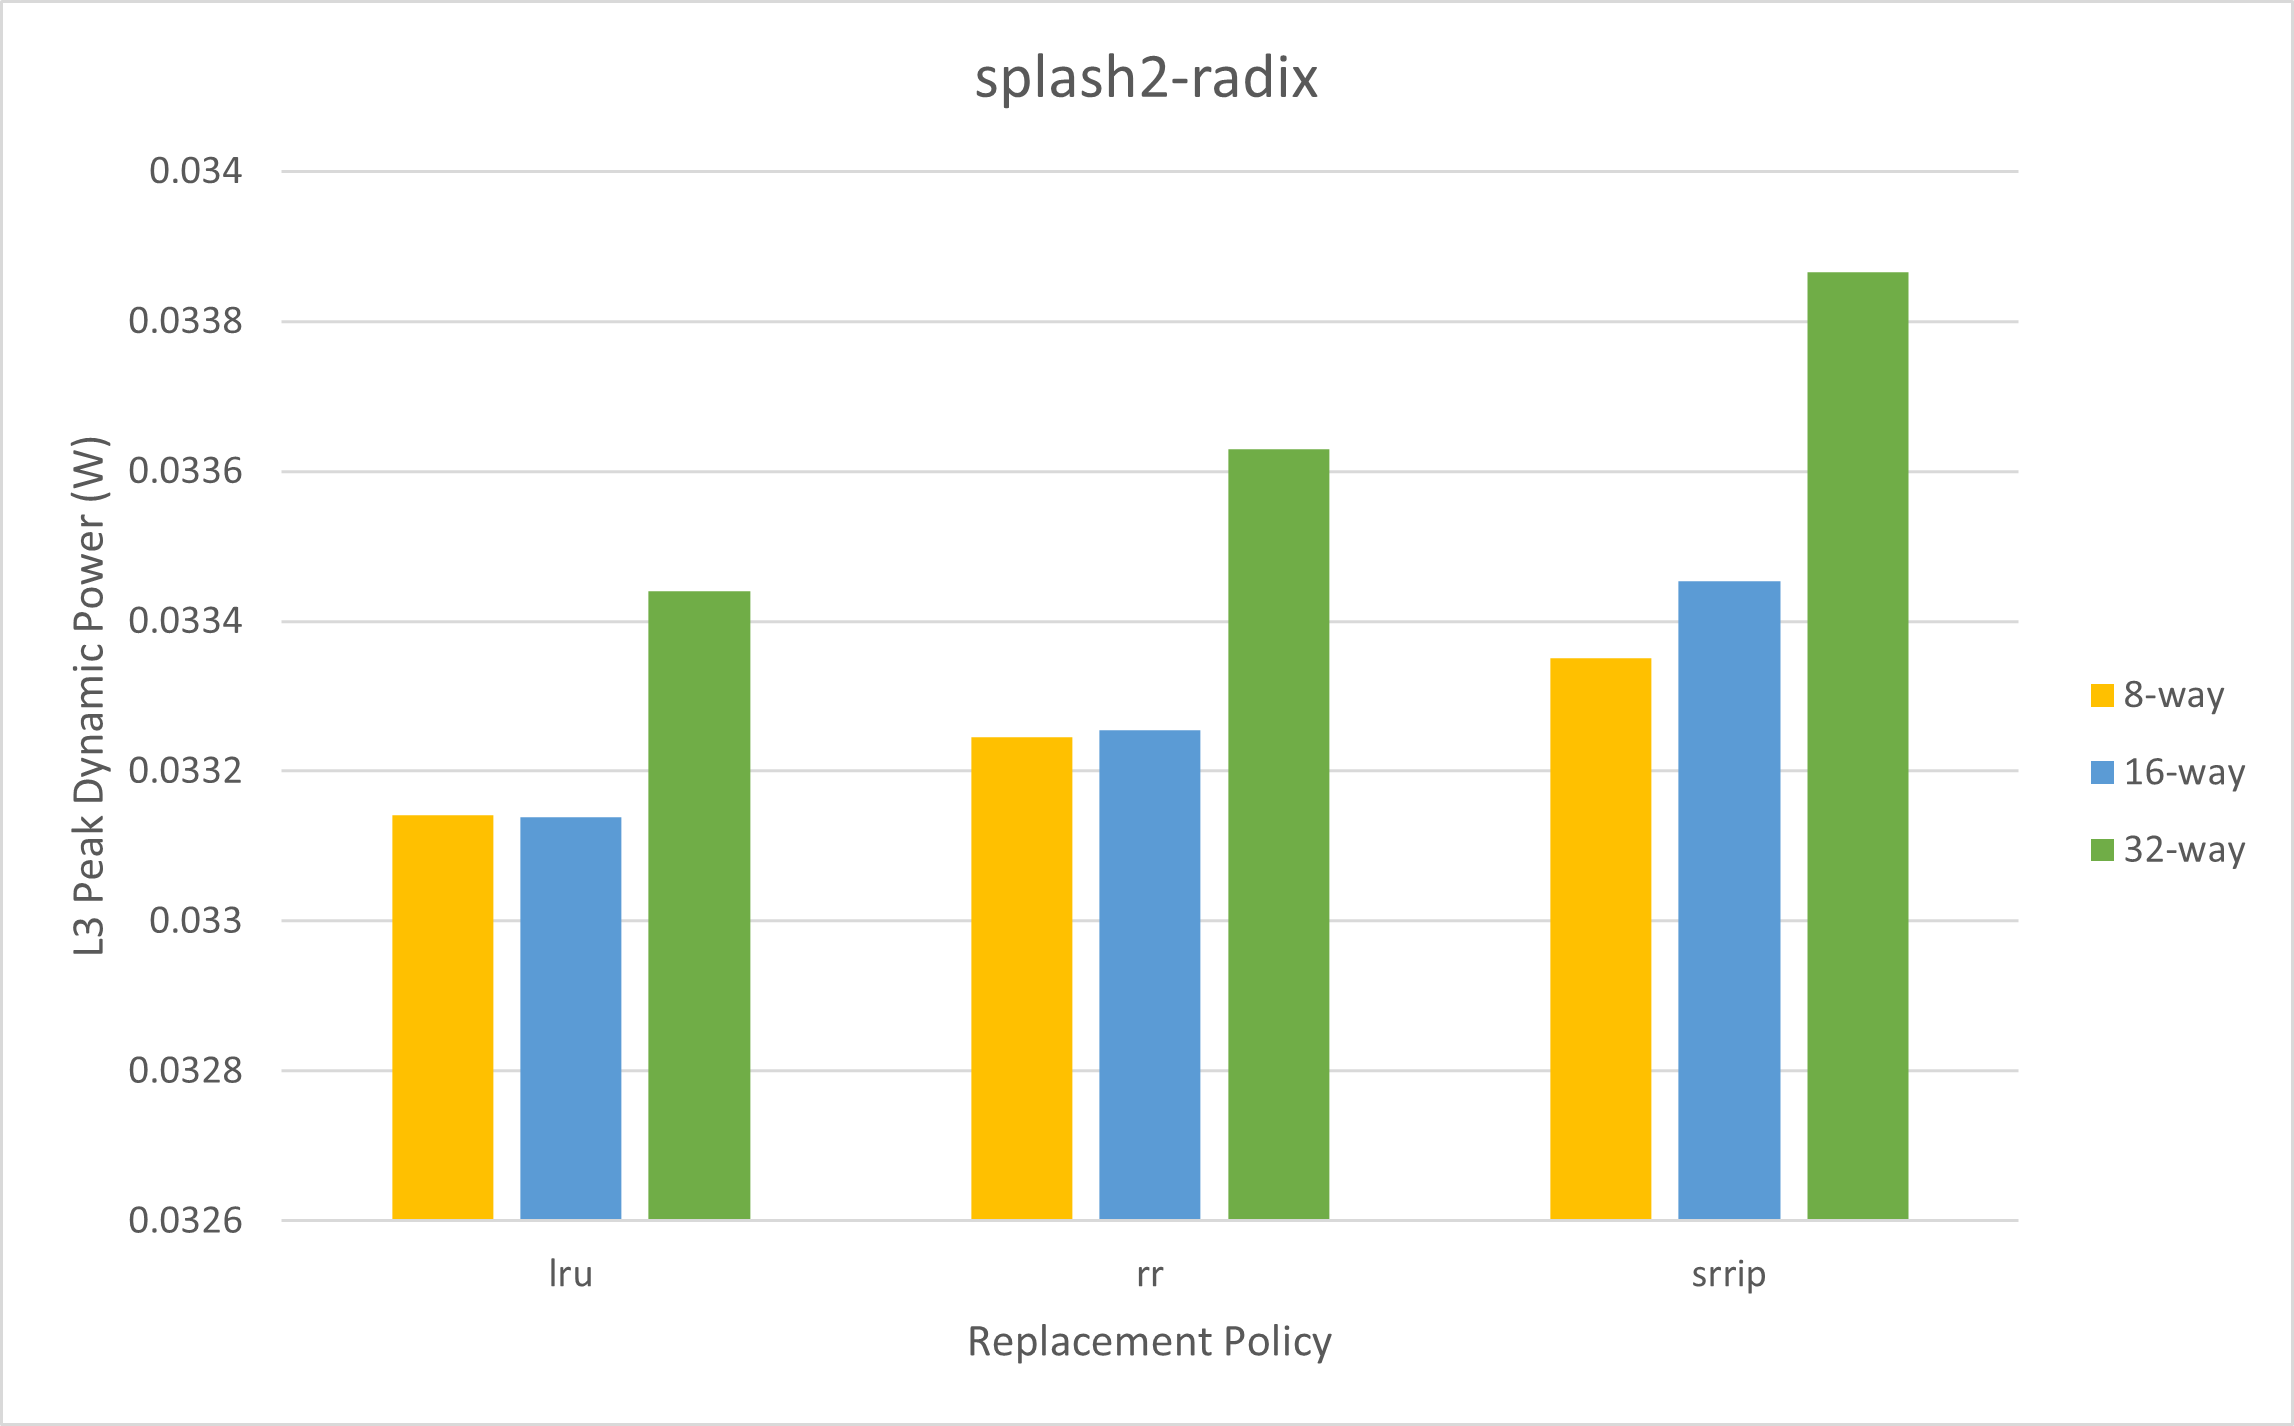
\includegraphics[width=1\textwidth]{./radixPeakDynamics.png}
                    \caption{}
                    \label{L3Peak:radix}
                \end{subfigure} &
                \begin{subfigure}{0.42\textwidth}
                    \centering
                    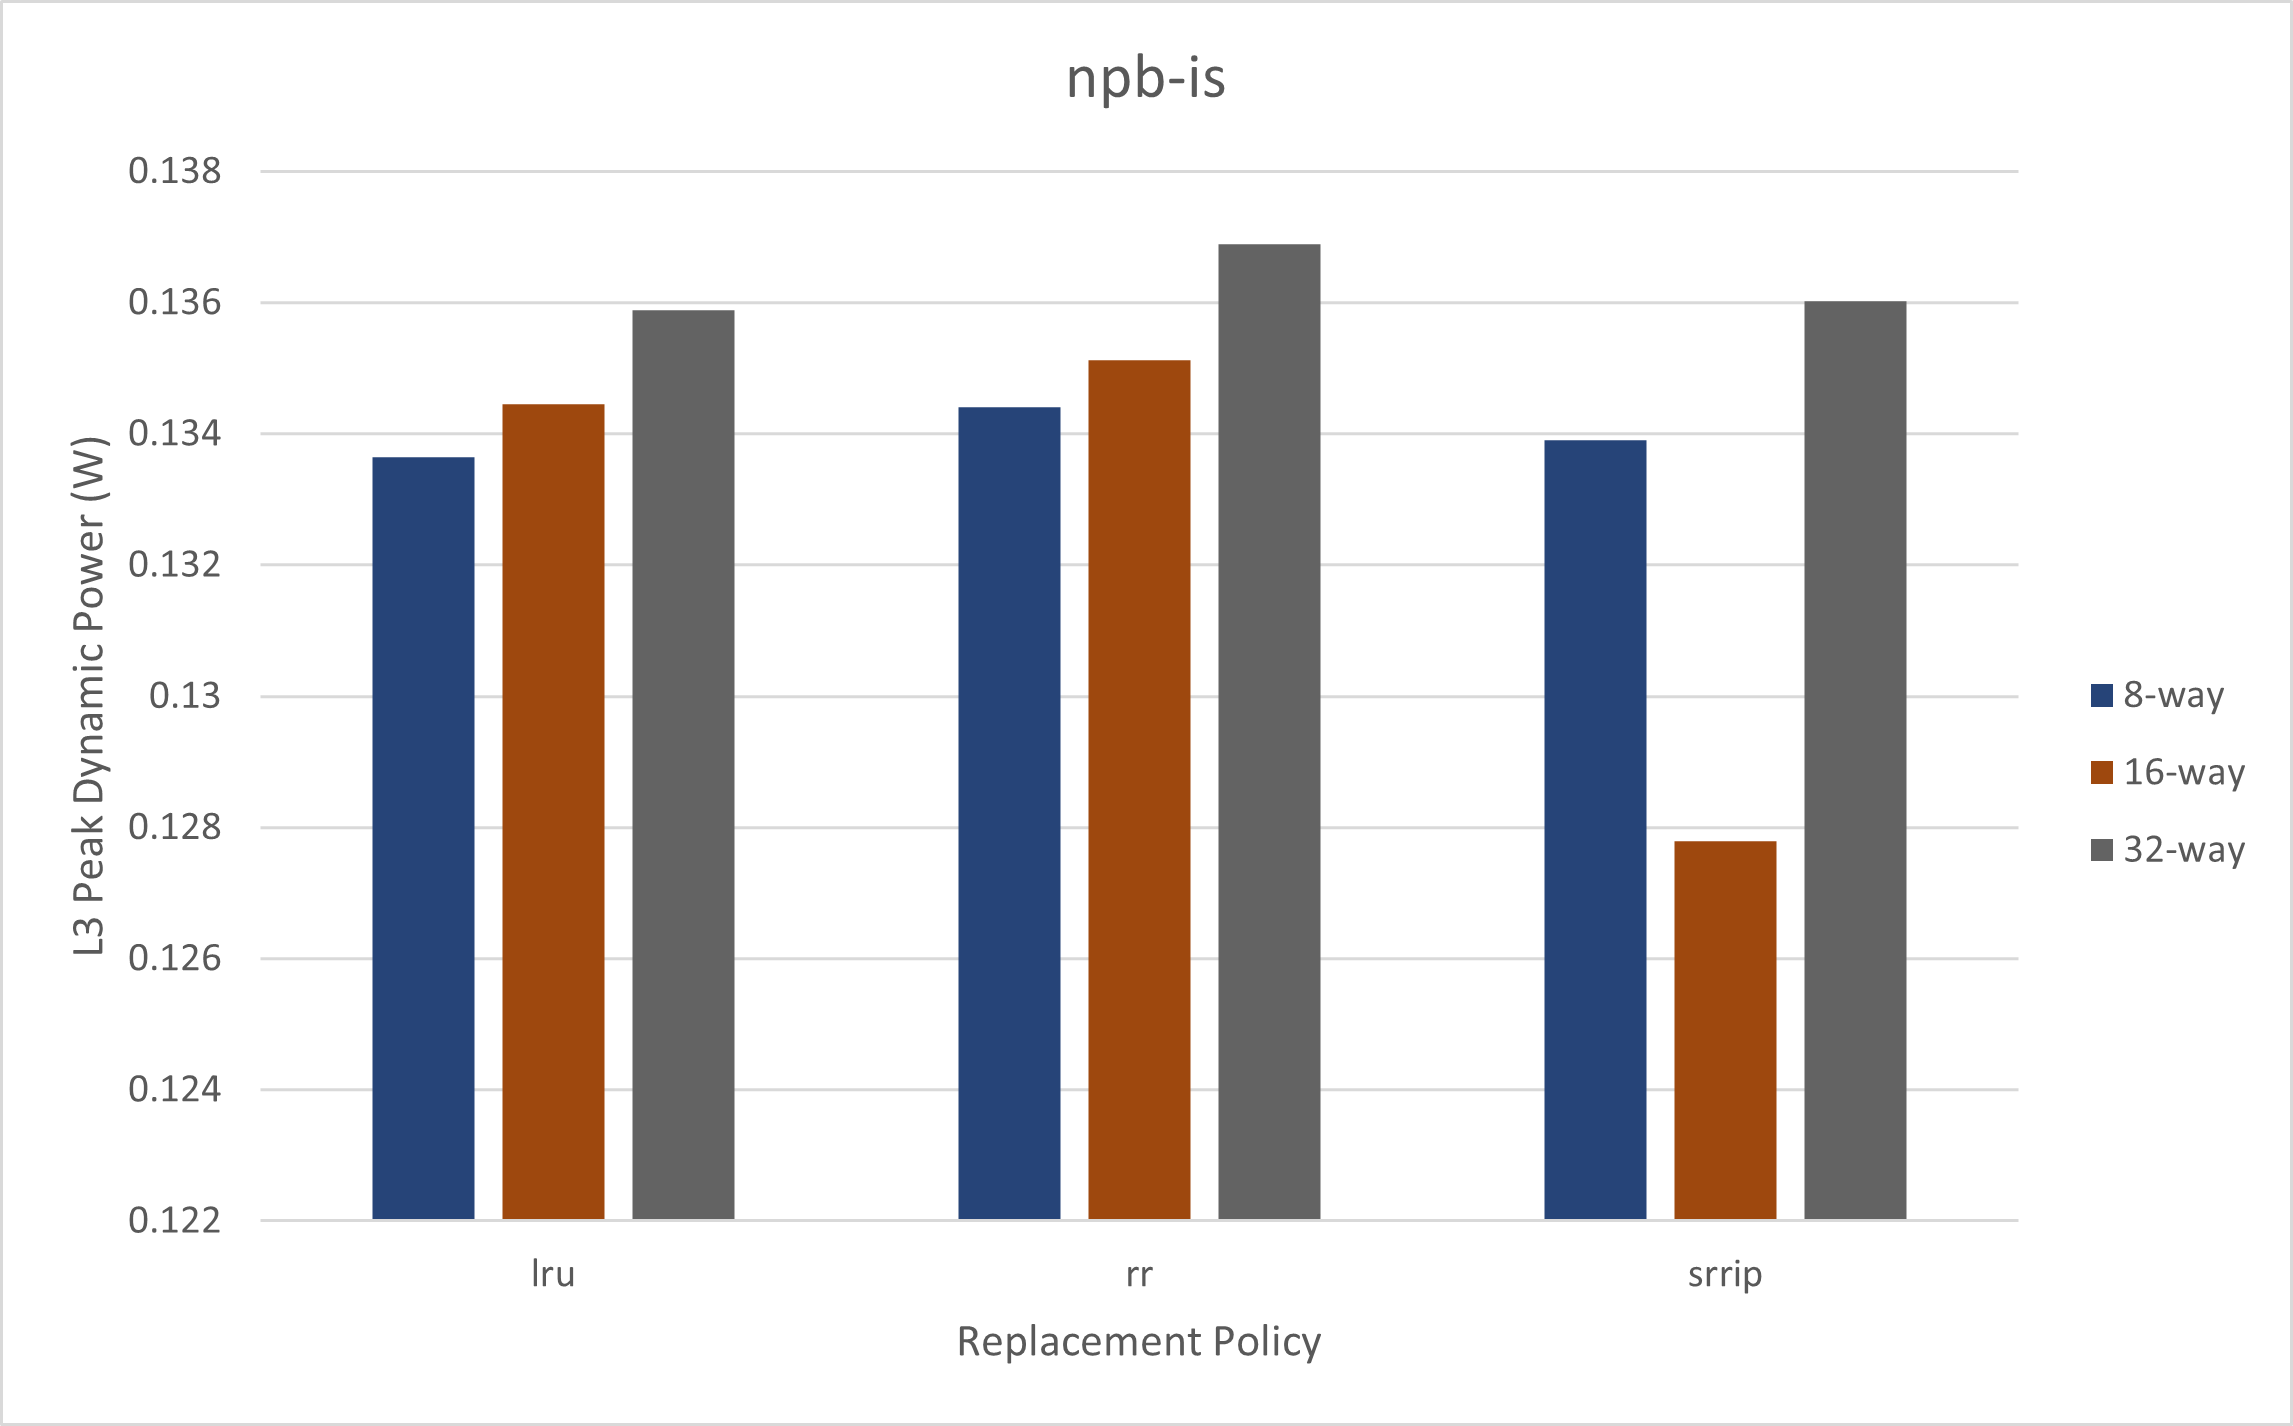
\includegraphics[width=1\textwidth]{./isPeakDynamics.png}
                    \caption{}
                    \label{L3Peak:is}
                \end{subfigure} 
            \end{tabular}\end{adjustwidth}
            \caption{Peak Dynamic Power of L3 cache across the L3 sweep.}
            \label{fig:peakDynamicL3}
        \end{figure}
        
        For the \texttt{npb-is} SRRIP tests, it is seen that 16-way set associativity had lower peak dynamic power for both processor and L3 (Fig. \ref{ProcPeak:is} and \ref{L3Peak:is}) then either of the 8- and 32-way. Since this was only observed for \texttt{npb-is} for an L3 using SRRIP replacement policy, this may be unique to a re-reference interval prediction replacement policy for parallel test applications, and would better be served in sweeping more replacement policies or a wider range of L3 associativities. Alternatively, similar to how higher block sizes do not improve performance but can degrade it pass a certain point (\cite{book}, App. B), these results could also imply that power consumptions does not improve at too low or too high associativities. 

        A few consistent effects on energy consumption were seen by replacement policy choice. In particular, round robin, a simple policy implementation, showed lower peak dynamic power for processor and L3 (Fig. \ref{fig:peakDynamicProcessor}, \ref{fig:peakDynamicL3}). This was less conistently observed for the \texttt{npb-is} benchmark (Fig. \ref{ProcPeak:is}, \ref{fig:peakDynamicL3}). These results implies that the type of workload and cache associativity affects energy consumption more than these few policy choice.  

            \clearpage

    \subsection{Performance Analysis: IPC}

        Fig. \ref{fig:IPC} shows that IPC is affected differently based on the test application swept. Replacement policy is not expected to affect IPC, however, Fig. \ref{IPC:ocean} and \ref{IPC:radix} also show that associativity does not affect it, either, for the \texttt{ocean.cont} and \texttt{radix} tests. Because this is not observed for \texttt{npb-is} (Fig. \ref{IPC:is}), this may again be due to the parallelism, because the mix of operations for \texttt{ocean.cont} and \texttt{radix} are sufficiently different (see CPI stacks in Fig. \ref{appfig:cpi:ocean:lru}, \ref{appfig:cpi:radix:lru}). For the parallel workload, IPC slightly improves with increased associativity; another exception is observed for the \texttt{npb-is} workload with an SRRIP L3 cache, in which the 16-way associativity has lower IPC than either the 8- or 32-ways. This aligns with the previously observed lower energy consumption for \texttt{npb-is} 16-way, SRRIP L3 cache test in Sec. \ref{sec:energy}, since fewer instructions execute per clock in this particular scenario.  

        Interestingly, Fig. \ref{fig:all:IPC} shows \texttt{npb-is} had higher IPC than \texttt{radix}, which itself has higher IPC than \texttt{ocean.cont} across all sweeps. This difference is explained by the parallelism since the increased instruction count per clocks comes from more executing at the same time, compared to \texttt{ocean.cont} and \texttt{radix}, which are not tuned for parallelism. 

    \begin{figure}[htb!]
        \begin{adjustwidth}{-2.75cm}{}\begin{tabular}{ccc}
            \begin{subfigure}{0.42\textwidth}
                \centering
                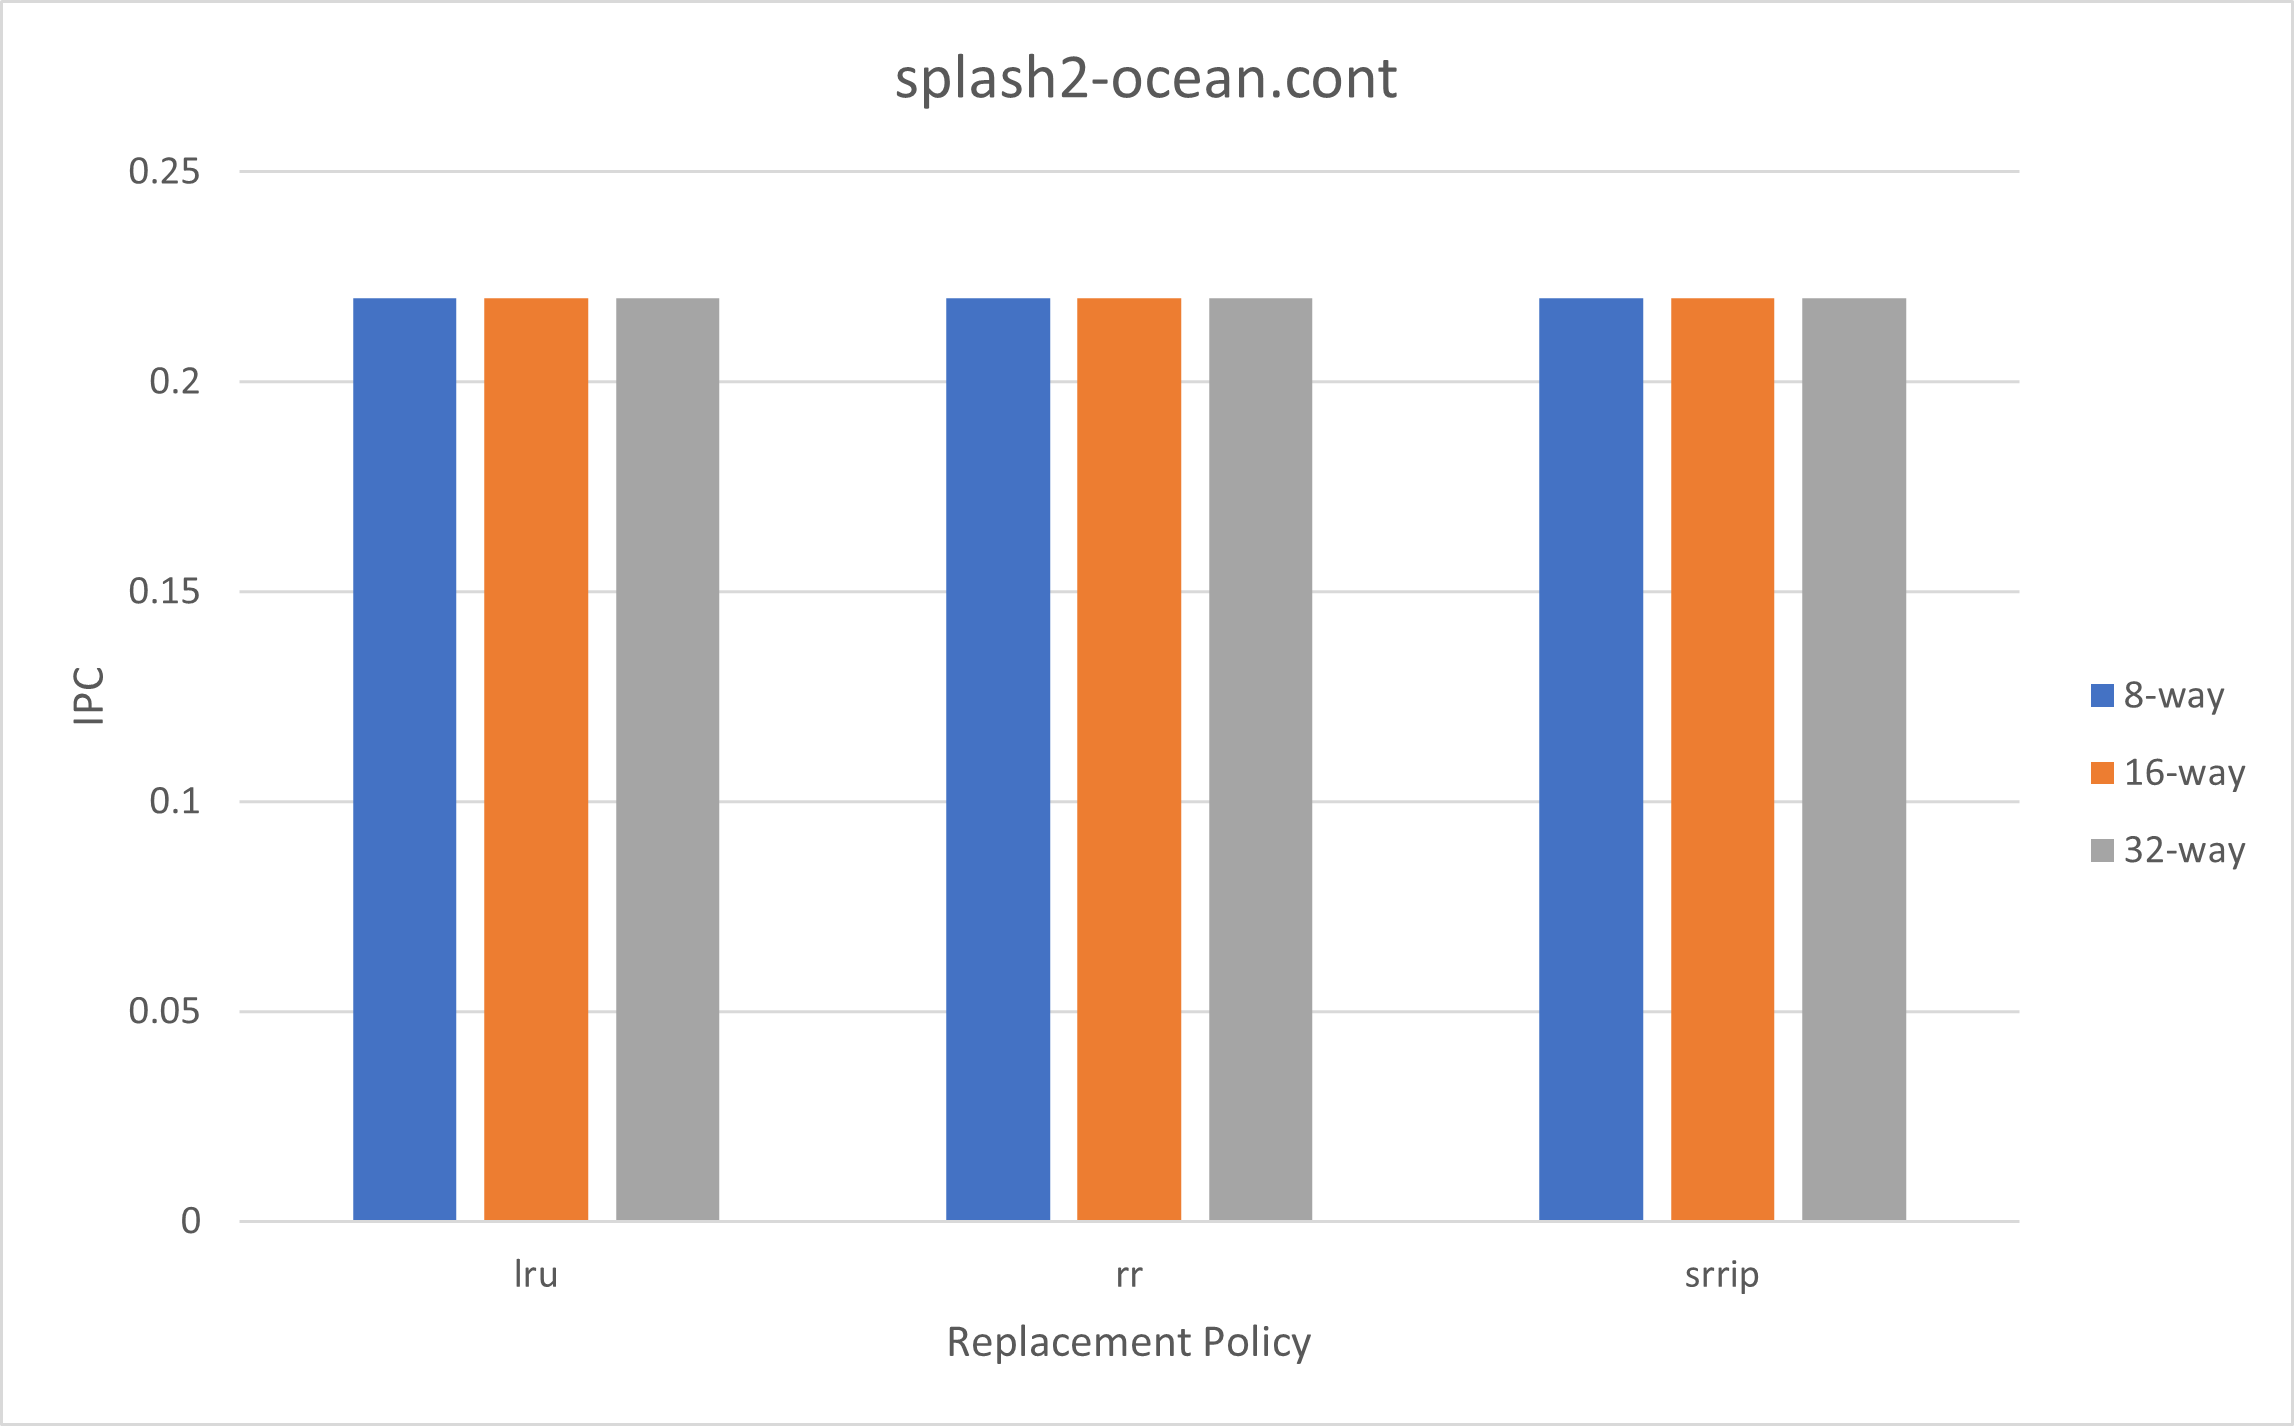
\includegraphics[width=1\textwidth]{./oceanIPC.png}
                \caption{}
                \label{IPC:ocean}
            \end{subfigure} &
            \begin{subfigure}{0.42\textwidth}
                \centering
                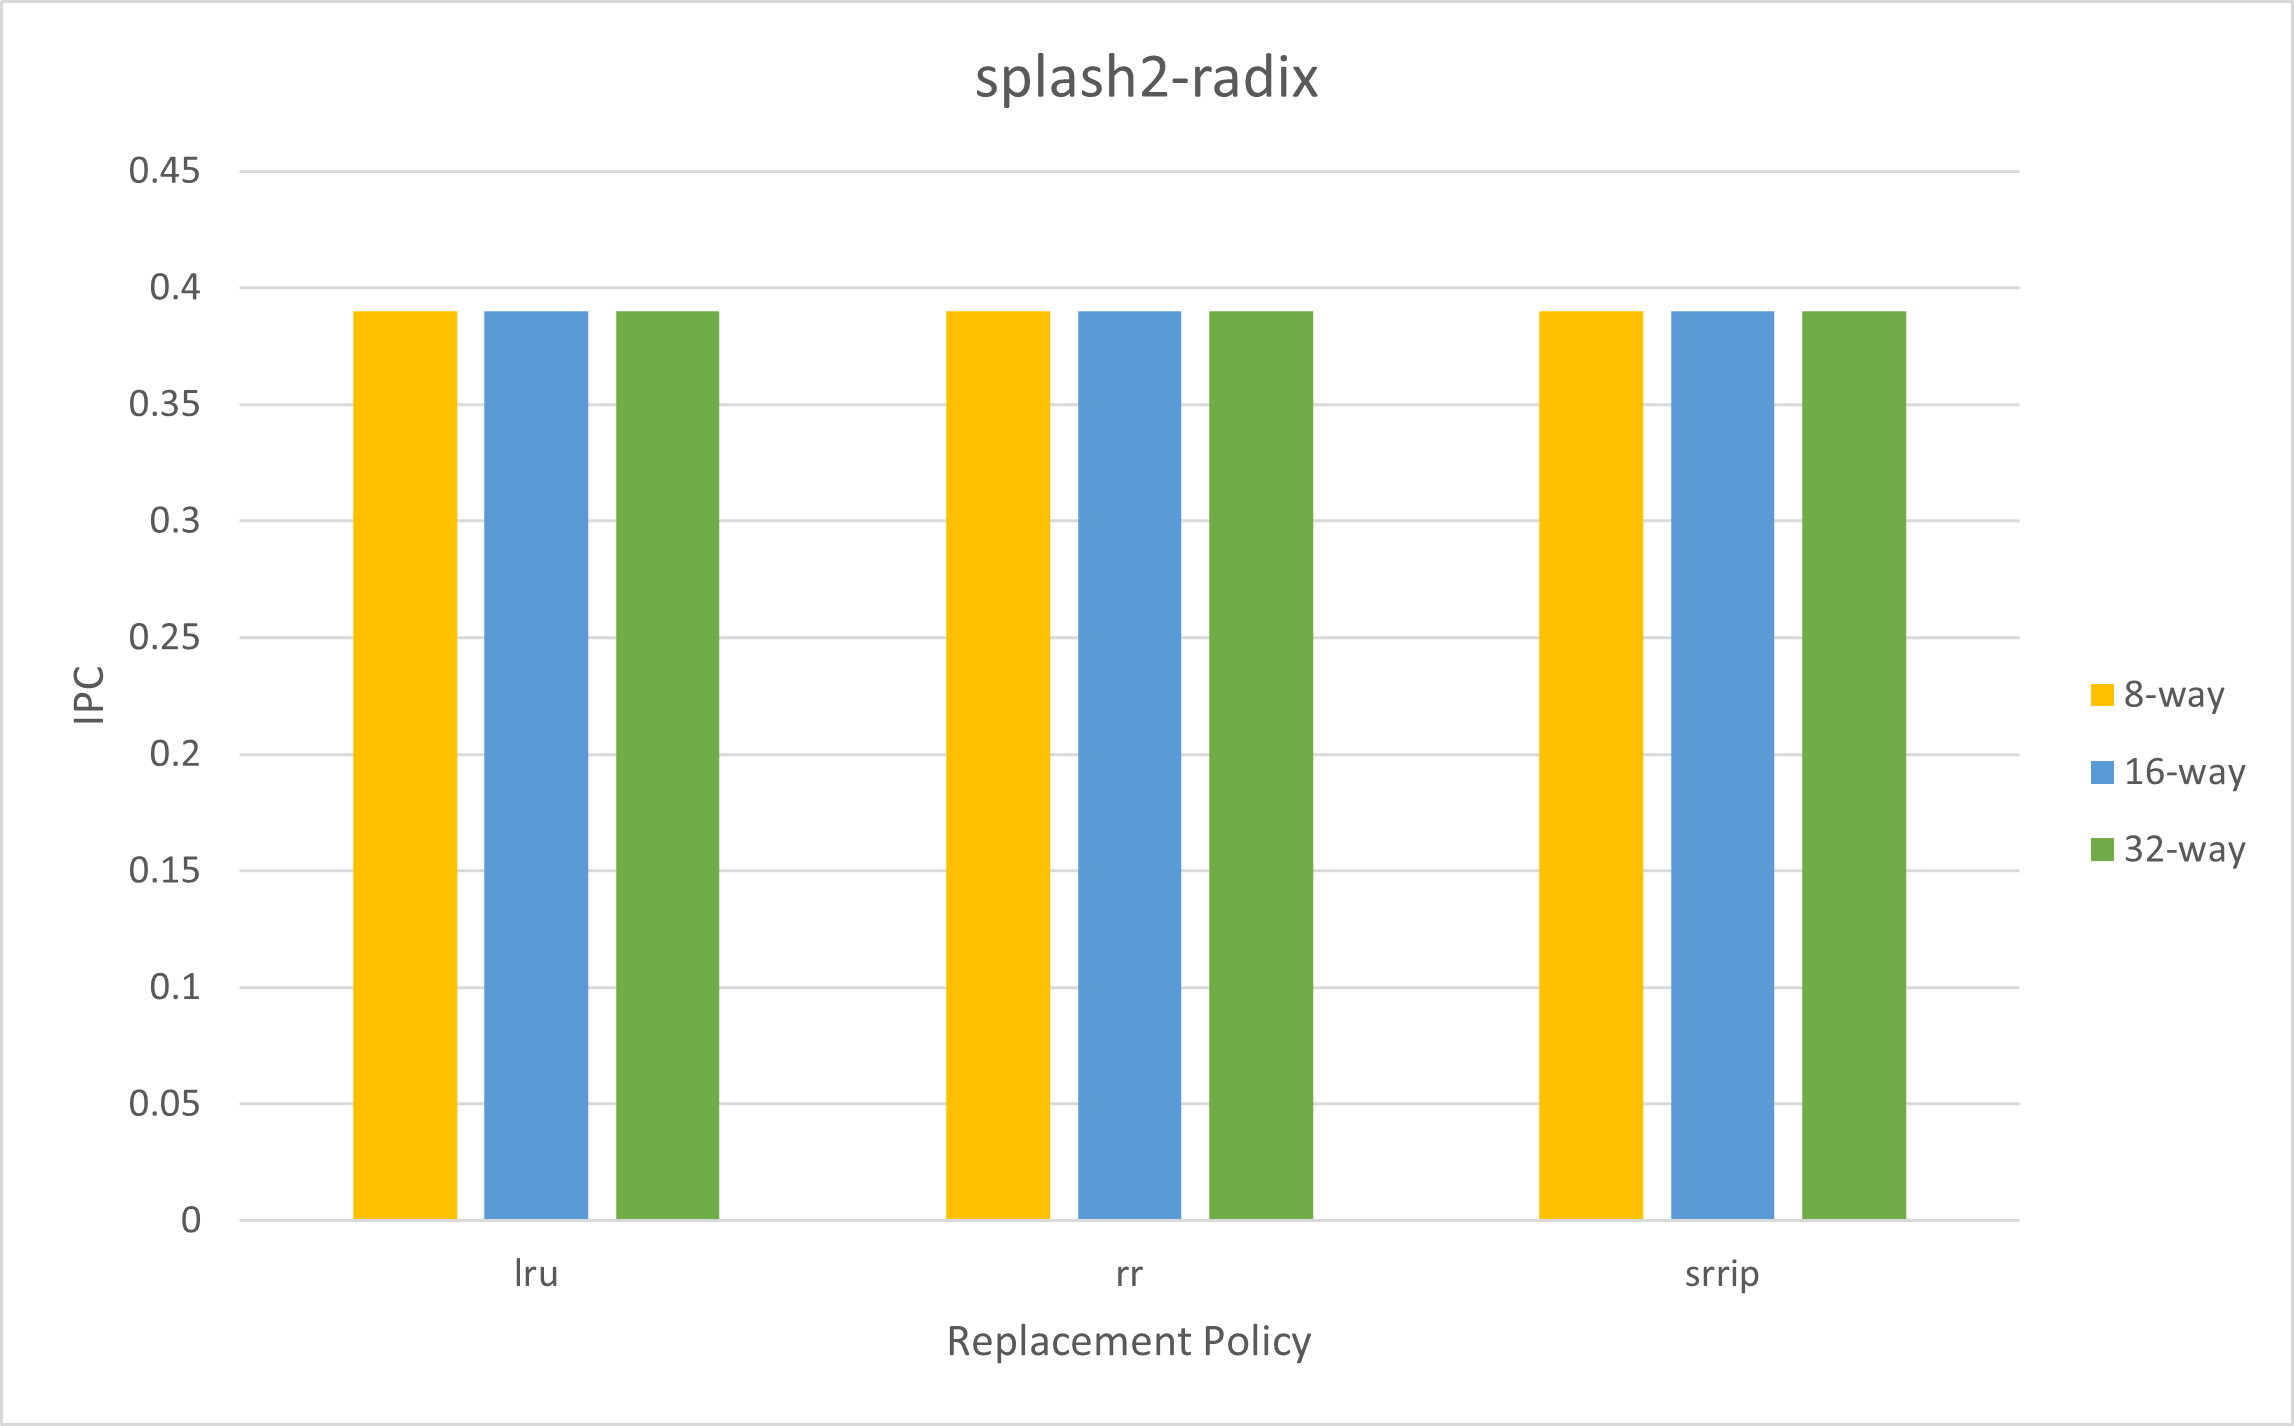
\includegraphics[width=1\textwidth]{./radixIPC.png}
                \caption{}
                \label{IPC:radix}
            \end{subfigure} &
            \begin{subfigure}{0.42\textwidth}
                \centering
                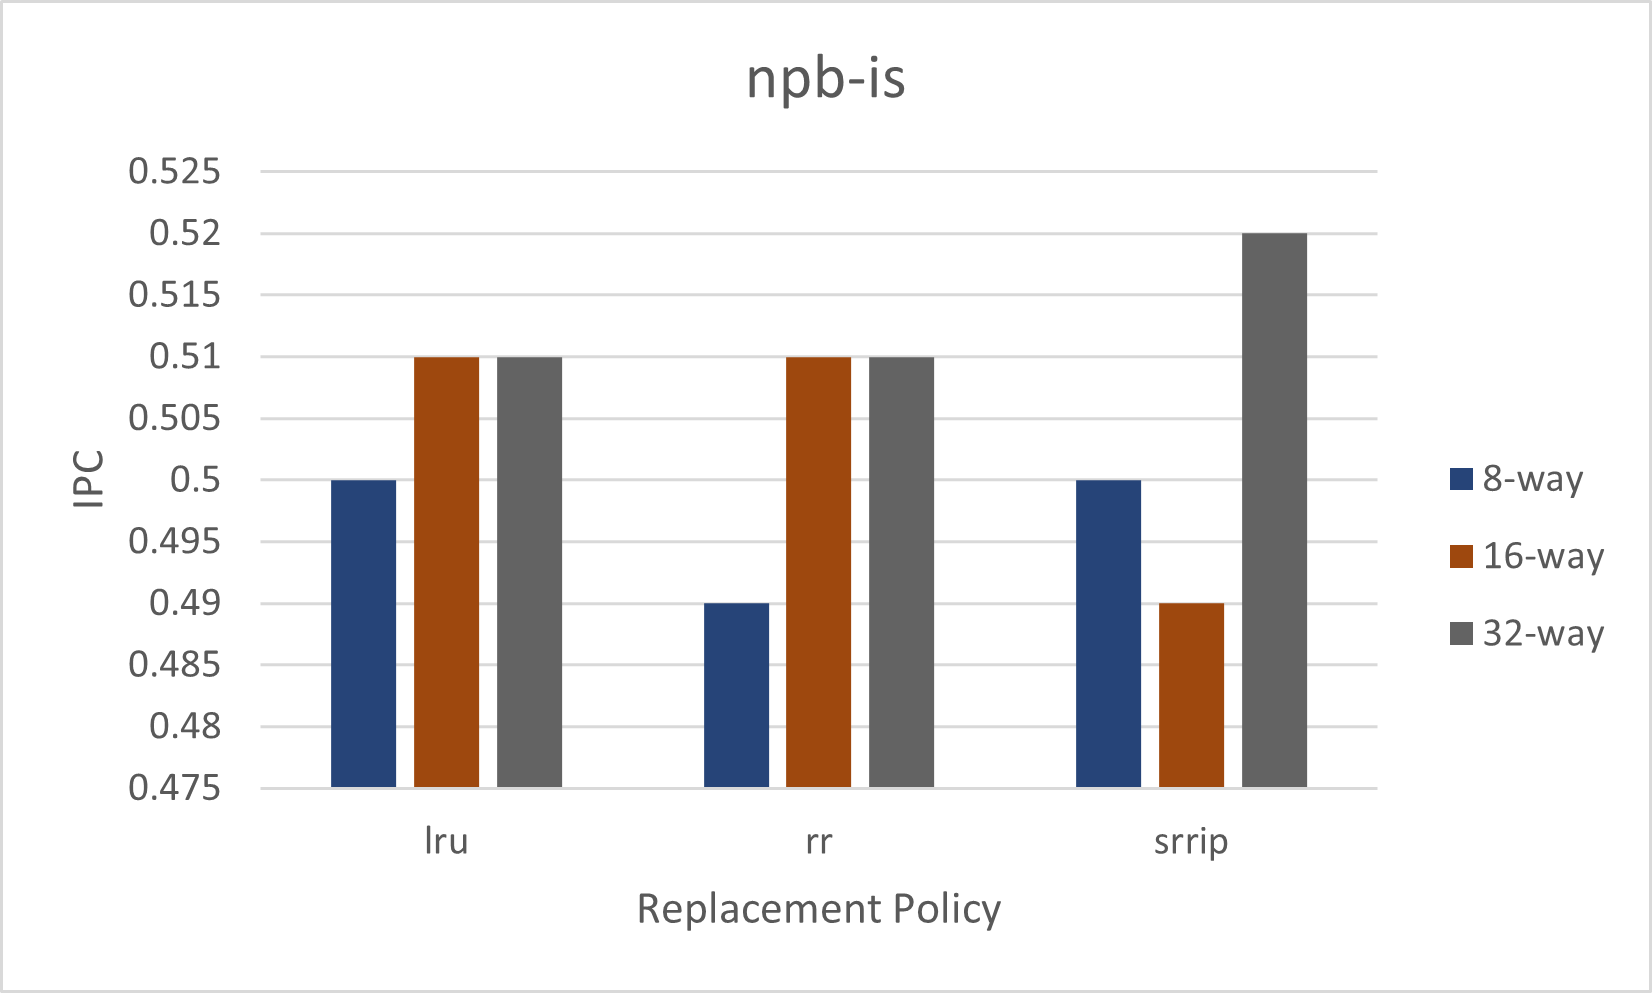
\includegraphics[width=1\textwidth]{./isIPC.png}
                \caption{}
                \label{IPC:is}
            \end{subfigure} 
        \end{tabular}\end{adjustwidth}
        \caption{IPC across the L3 sweep in separate benchmarks.}
        \label{fig:IPC}
    \end{figure}

    \begin{figure}[htb!]
        \centering
        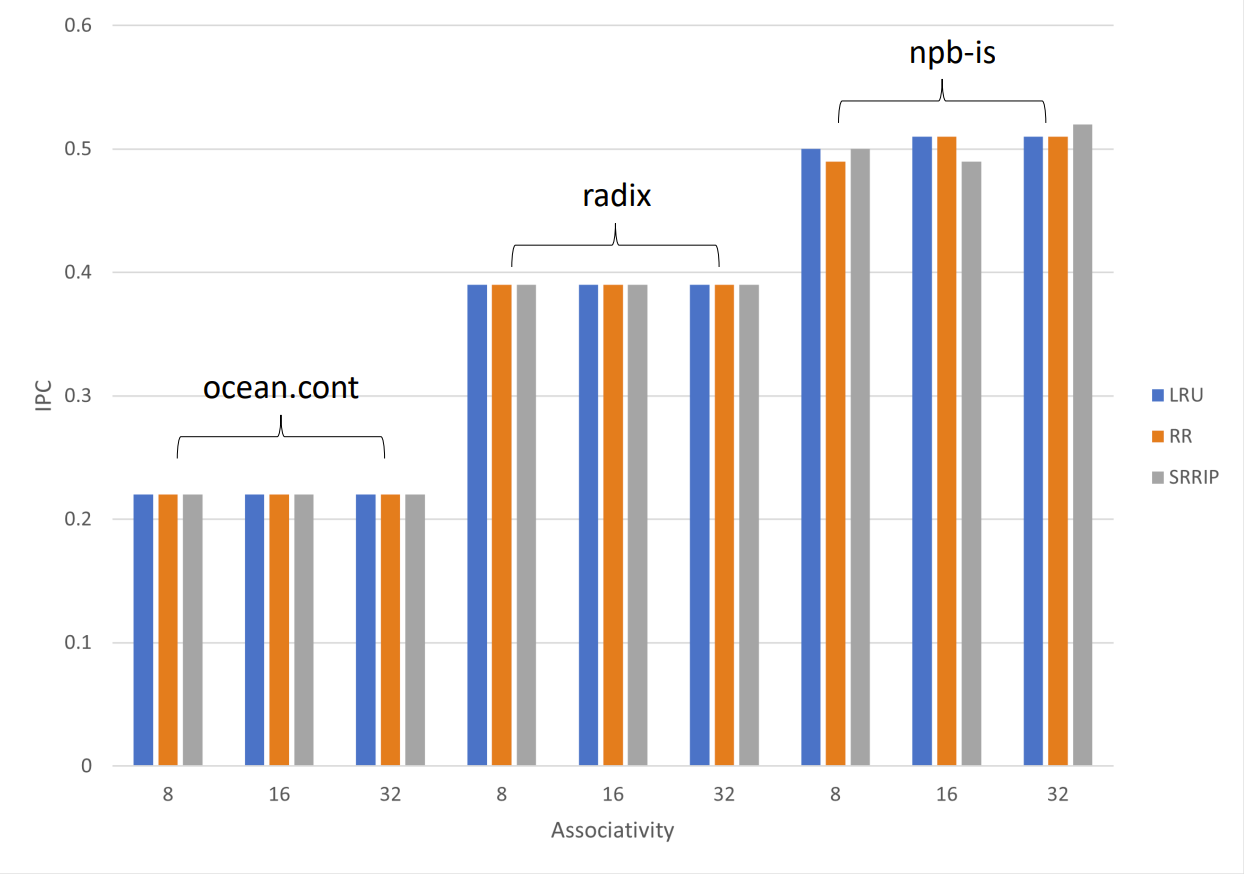
\includegraphics[width=0.6\textwidth]{./allIPClabeled.png}
        \caption{L3 cache associativity and replacement policy graphed against \textbf{IPC} for all three benchmarks. }
        \label{fig:all:IPC}
    \end{figure}

    \clearpage

    \subsection{Performance Analysis: Miss Rate}
        Fig. \ref{fig:Miss} shows that miss rate improves with higher associativity. This is because with more blocks in each set, this lowers the chance of conflict misses when memory accesses index to the same set (\cite{book}, Ch 2). However, this is also at the cost of 1) hit time, as more blocks are being searched in parallel for an access, and 2) higher power consumption (Sec. \ref{sec:energy}). When compared against each other, \texttt{npb-is} shows higher miss rate than either \texttt{ocean.cont} or \texttt{radix}; \texttt{radix} had the least memory access operations, and therefore expected to have the lowest miss rate. \texttt{nbp-is} is also more memory intensive than \texttt{ocean.cont}; despite parallelism previously shown to have helped with energy saving for overall power consumption and peak dynamic power in L3, it does not help the miss rate, as seen in how significantly higher the miss rate for \texttt{npb-is} is than for \texttt{ocean.cont} (Fig. \ref{fig:all:Miss}). 

        The type of workload also appears to have had miss rate affected differently by replacement policy. In particular, memory intensive \texttt{ocean.cont} and \texttt{npb-is} has lower miss rate with round robin, while \texttt{radix} has higher miss rate with round robin. This tells us that more complex replacement policies on memory intensive workloads are a detriment to performance, while simple replacement policies do not benefit the performance of applications with less memory access operations.


    \begin{figure}[htb!]
        \begin{adjustwidth}{-2.75cm}{}\begin{tabular}{ccc}
            \begin{subfigure}{0.42\textwidth}
                \centering
                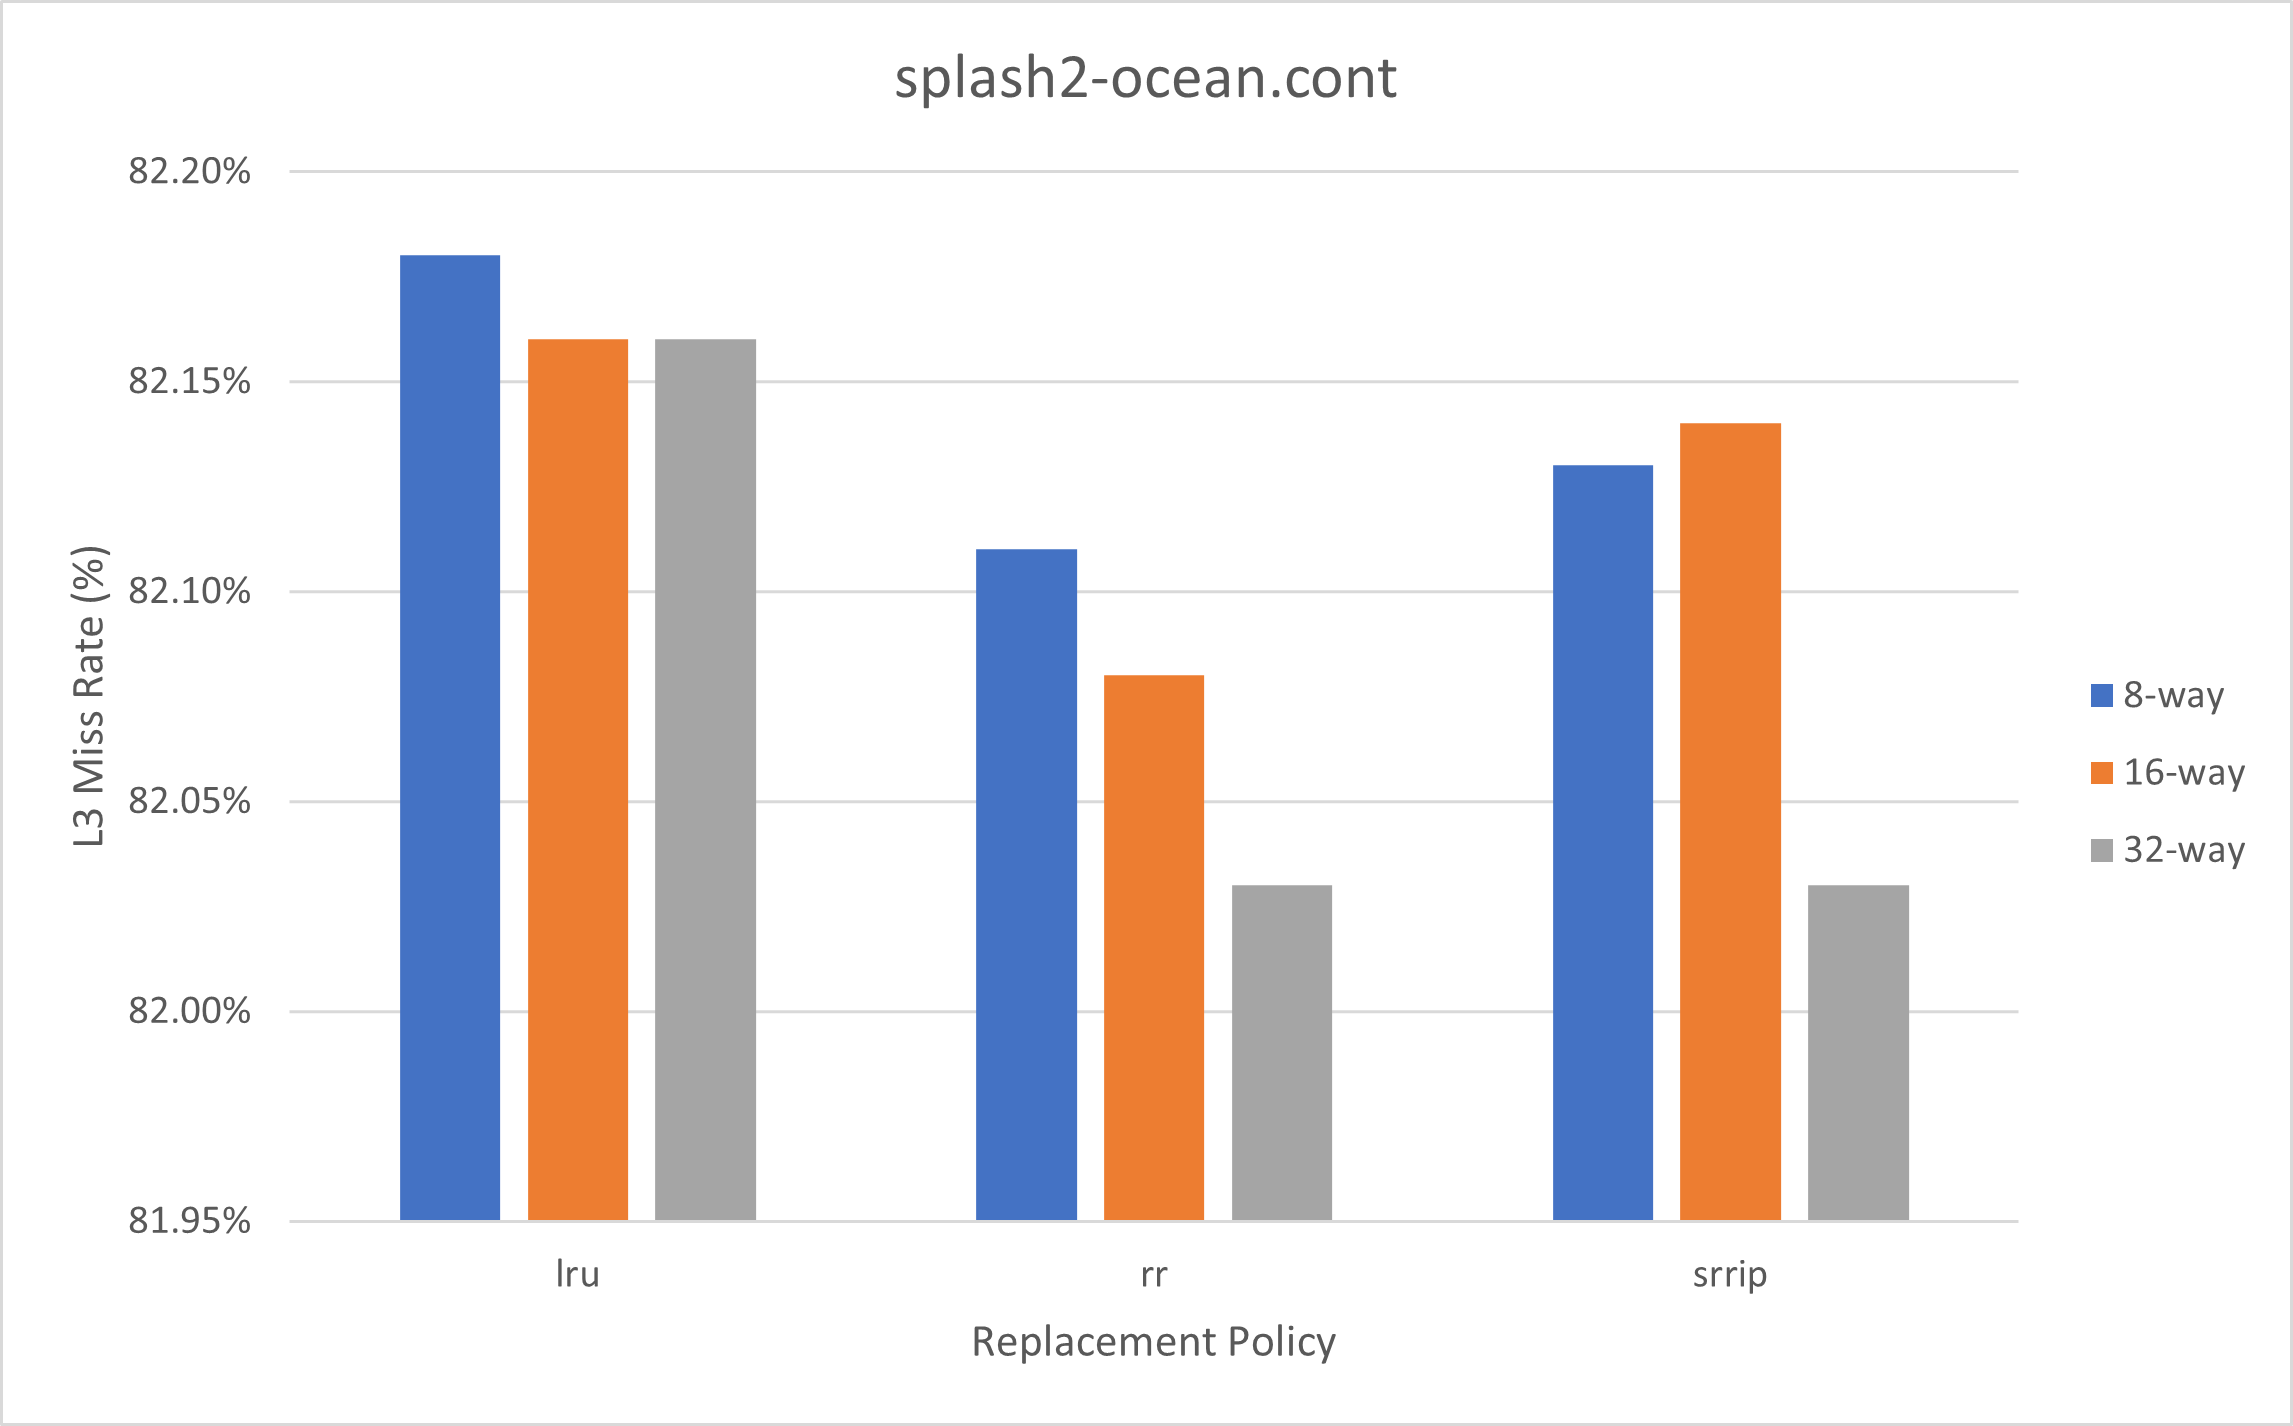
\includegraphics[width=1\textwidth]{./oceanL3Miss.png}
                \caption{}
                \label{Miss:ocean}
            \end{subfigure} &
            \begin{subfigure}{0.42\textwidth}
                \centering
                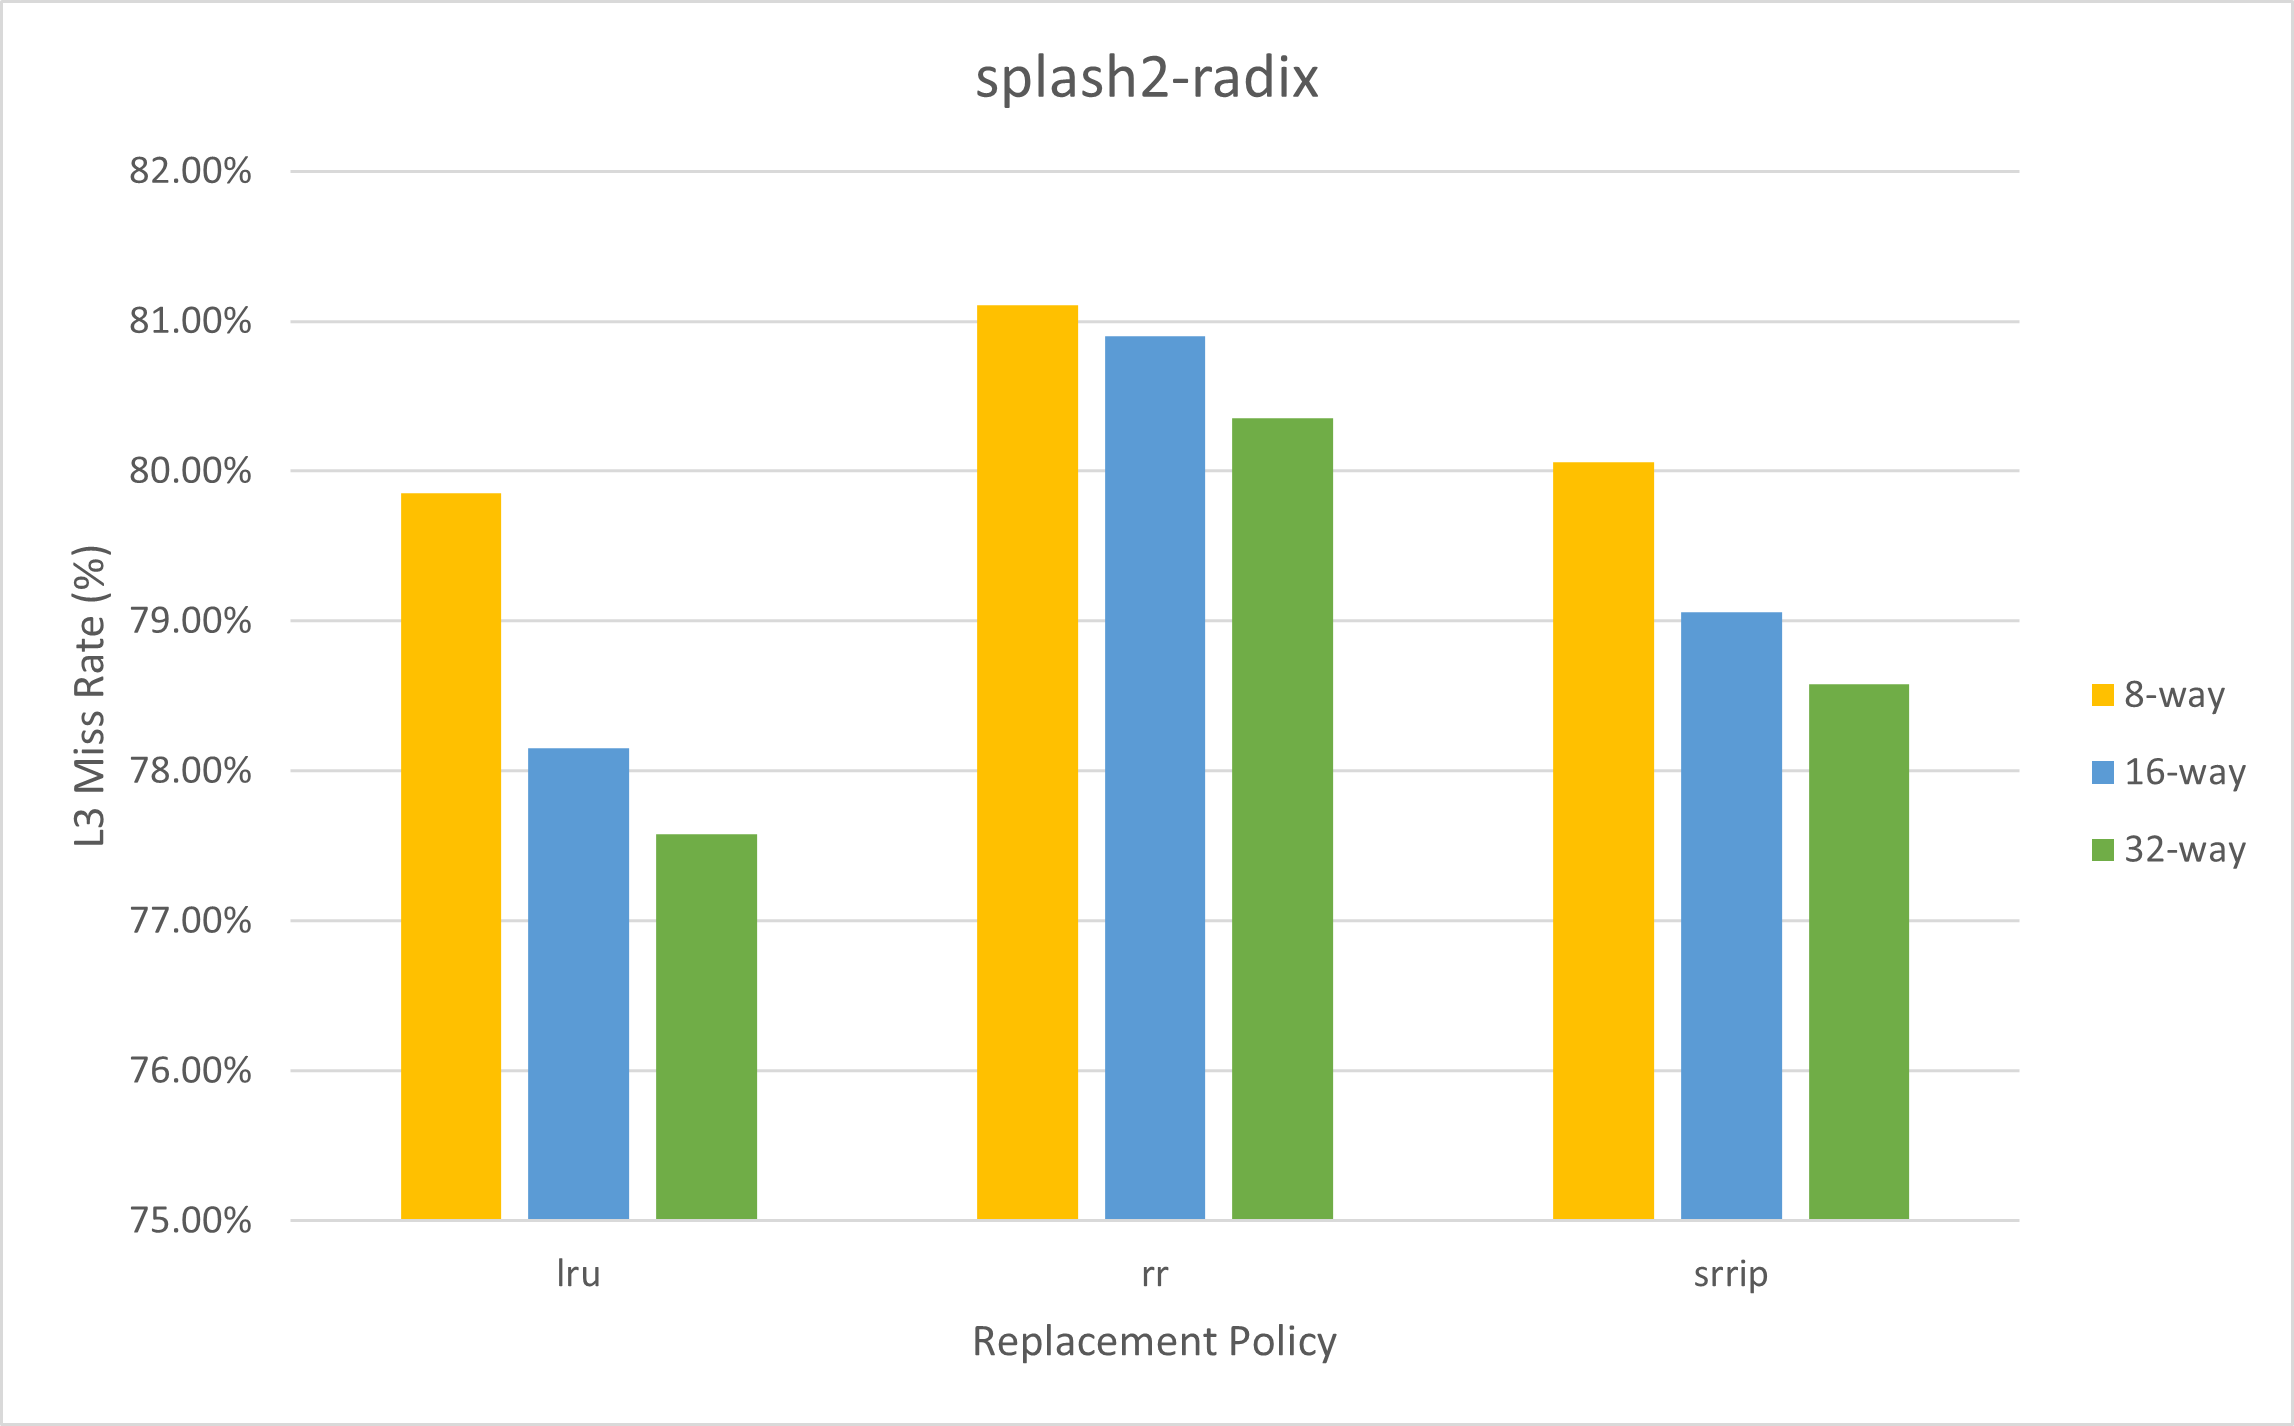
\includegraphics[width=1\textwidth]{./radixL3Miss.png}
                \caption{}
                \label{Miss:radix}
            \end{subfigure} &
            \begin{subfigure}{0.42\textwidth}
                \centering
                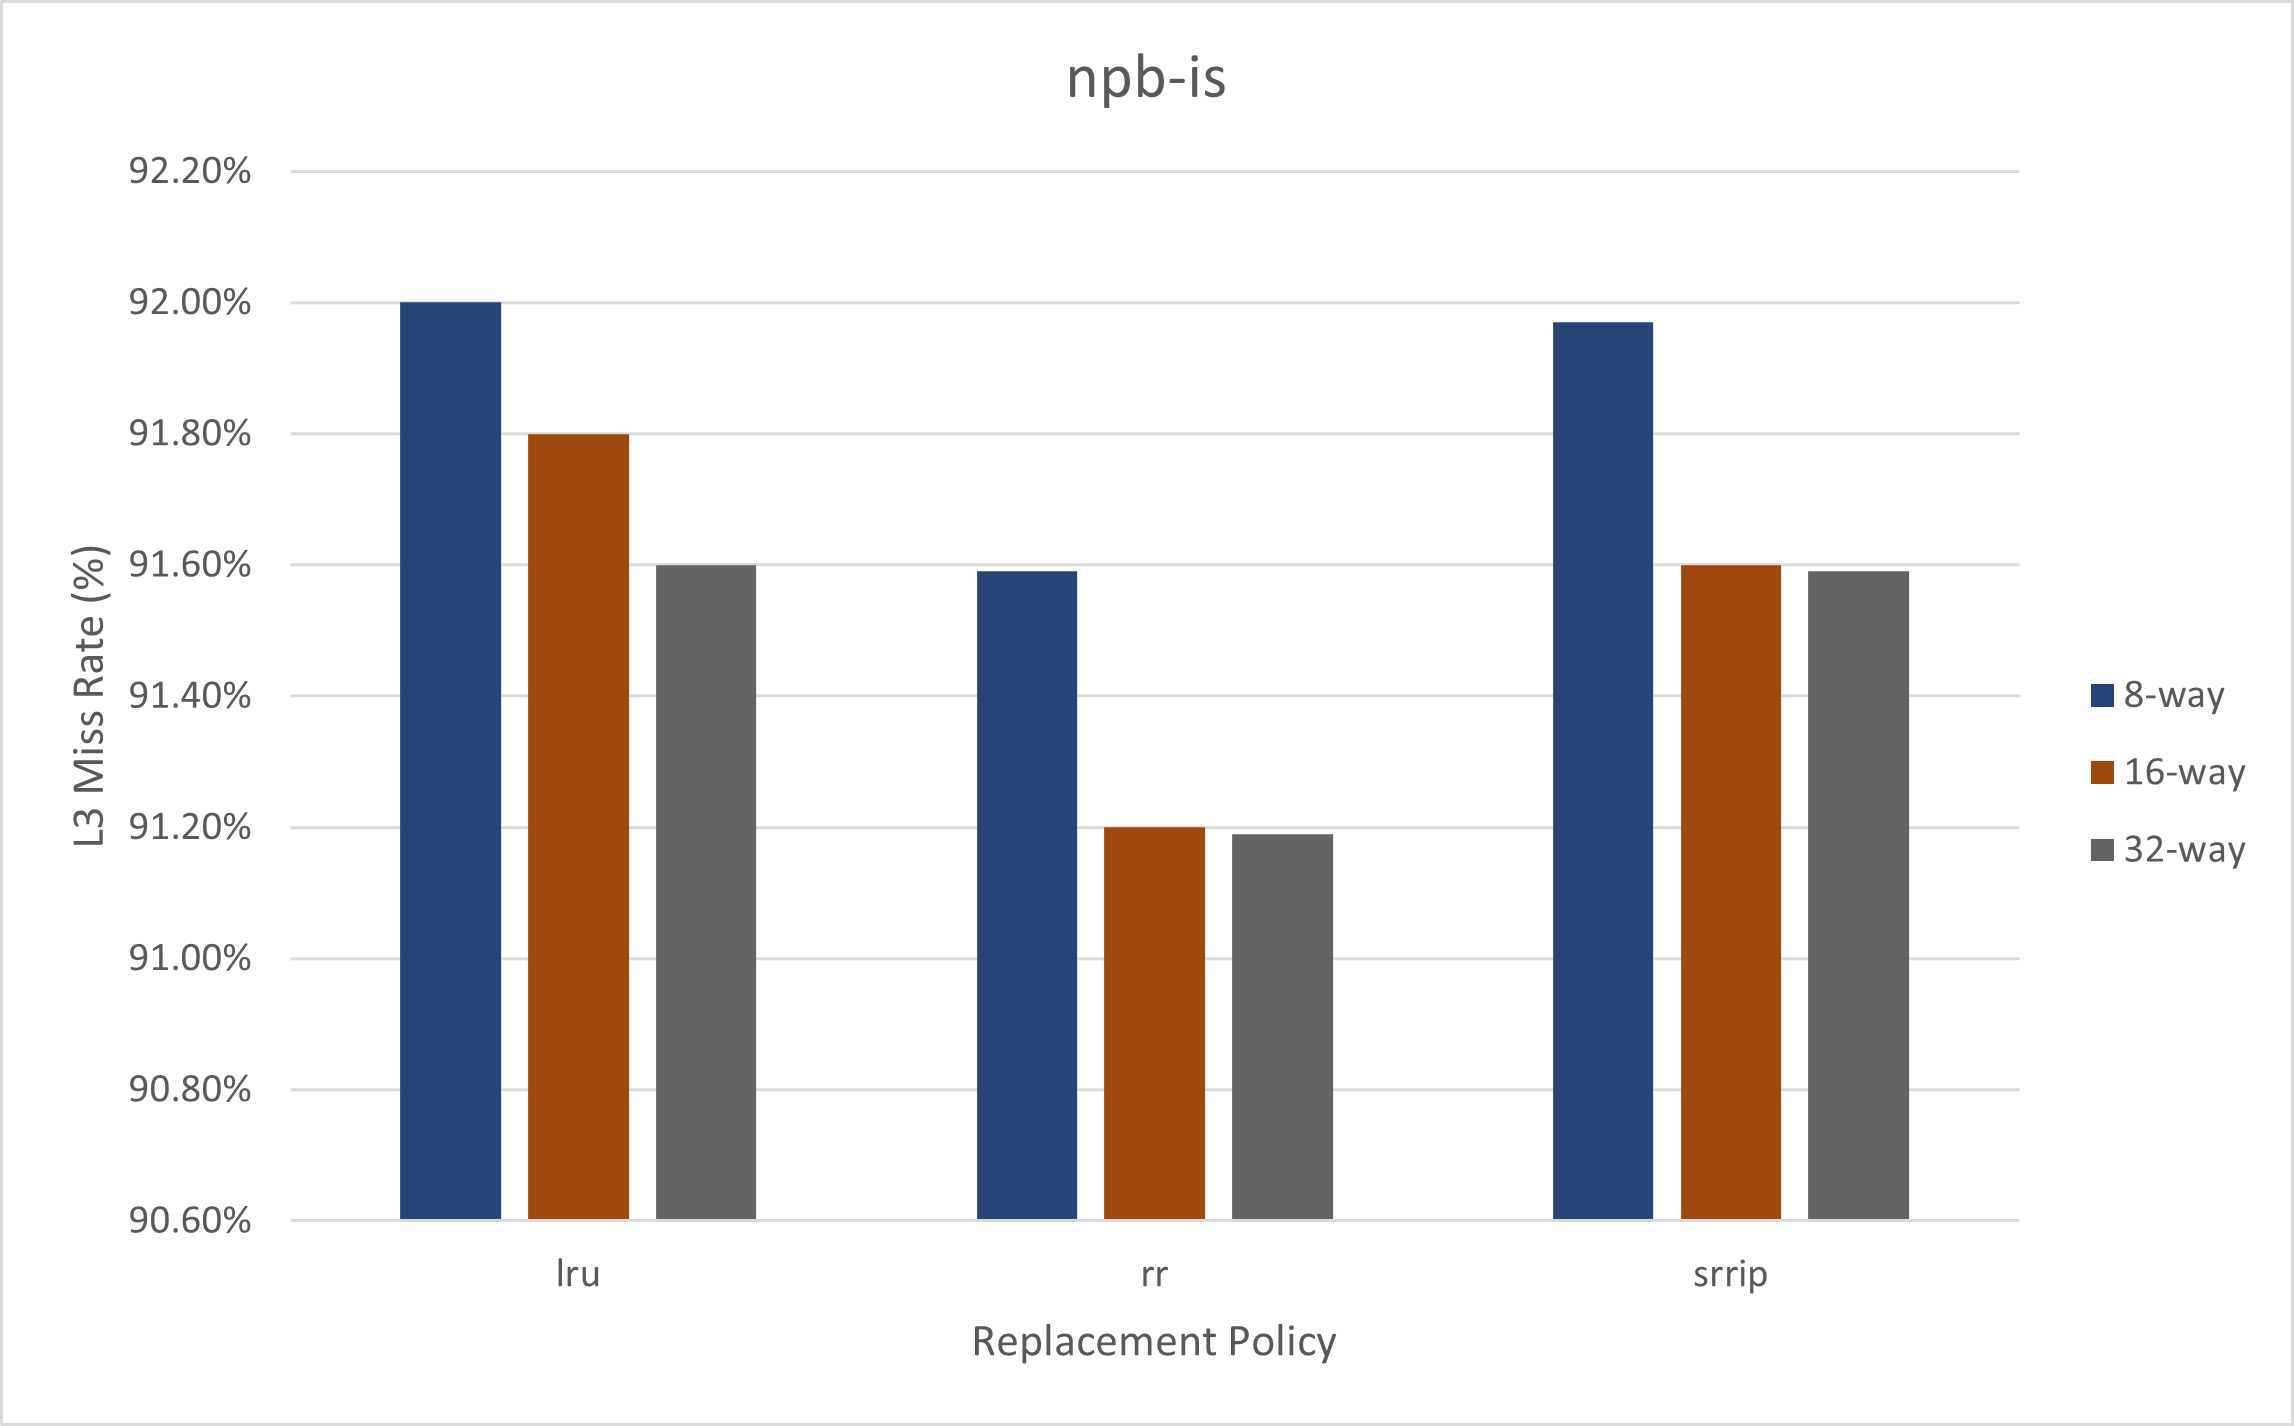
\includegraphics[width=1\textwidth]{./isL3Miss.png}
                \caption{}
                \label{Miss:is}
            \end{subfigure} 
        \end{tabular}\end{adjustwidth}
        \caption{Miss rate across the L3 sweep.}
        \label{fig:Miss}
    \end{figure}

    \begin{figure}[htb!]
        \centering
        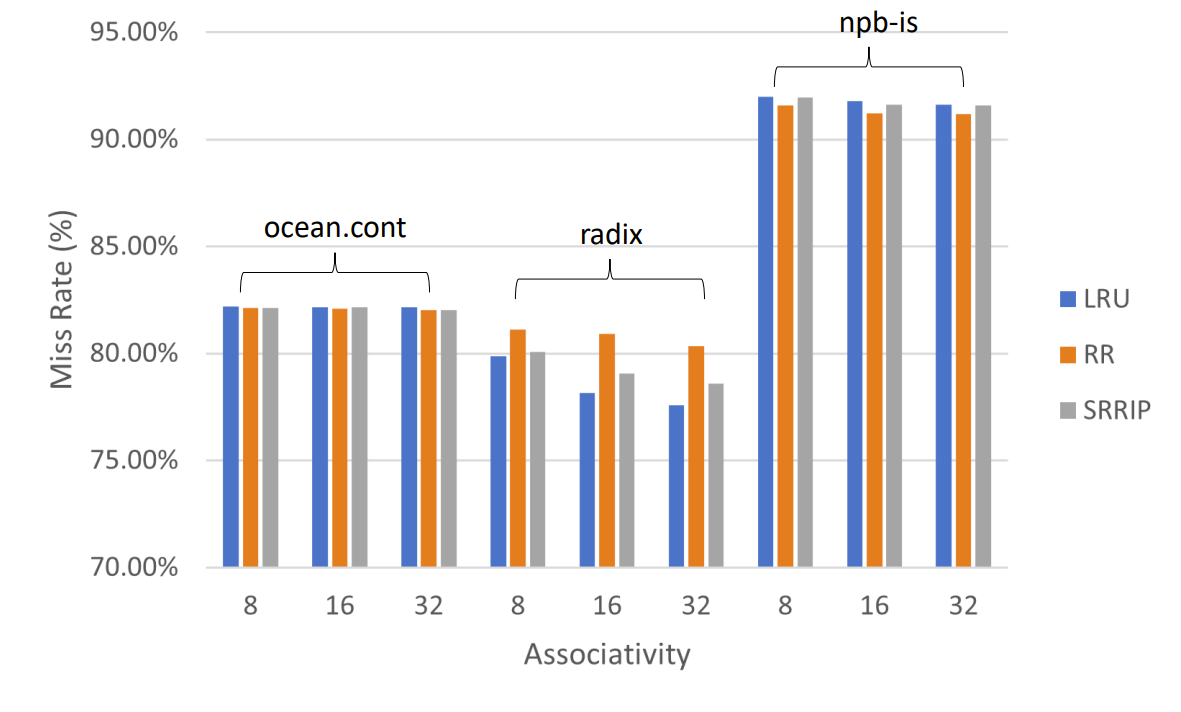
\includegraphics[width=0.8\textwidth]{./allMisslabeled.png}
        \caption{L3 cache associativity and replacement policy graphed against \textbf{miss rate} for all three benchmarks. }
        \label{fig:all:Miss}
    \end{figure}
    \clearpage


    \section{Conclusion}

        Sweeping the associativity and replacement policy of a unified last level cache show interesting effects on energy consumption and performance. While there were not huge differences in energy consumption in individual benchmarks while varying associativity and replacement policy, some of the trends of increased power were consistent with increasing associativity. More evident was that miss rate did decrease with associativity increasing. Surprisingly, IPC was not impacted by either sweeps, and those seen in the pallel application was inconsistent. And while it was clear that more memory intensive workloads (\texttt{ocean.cont} and \texttt{npb-is}) costed more in terms of energy and performance, we did observe unexpected results in the memory intense parallel benchmark, which showed that parallelism had some energy saving benefits but did not improve in miss rates for more memory intensive operations. If time permitted, this experiment could be expanded upon to included a wider range of replacement policies and associativity. I would expect to see too low and too high associativity to degrade memory performance. And we would sweep aditional parallel workloads, and those with more diverse sets of operations, given variance in the data observed for \texttt{npb-is}; it would be interesting to see if other workloads yield similar deviations or reveal new trends. 


        % Memory intense benchmarks consumed more energy, but individually, there was not a huge impact on individual work loads if we vary associativity and policy. 

        % Surprisingly. IPC was not impacted by associativity or replacement policy

        % Parallelism is a contributing factor that affects outcome of performance 

        % Miss rate generally decreases with higher associativity, but higher energy consumption was seen 



    \clearpage
    %%%%%%%%%%%%%%%%%%%%%%%%%%%%%%%%%%%%%%%%%%%%%%%%%%%%%%%%%%%%%%%%%%%%%%%%

    \section{Appendix: Raw Post Processed Data}
    \label{appendix:raw}

    \subsection{npb-is} %%%%%%%%%%%%%%%%%%%%%%%%%%%%%%%%%%%
        
        \subsubsection{Power Results} %%%%%%%%%%%%%%%%%%%%%%%%%%%%%%%%%%%

        % LRU
        \begin{figure}[hbt!]
            \centering 
            \begin{adjustwidth}{-2.75cm}{}
            \begin{tabular}{ccc}
                \begin{subfigure}{0.42\textwidth}
                    \centering
                    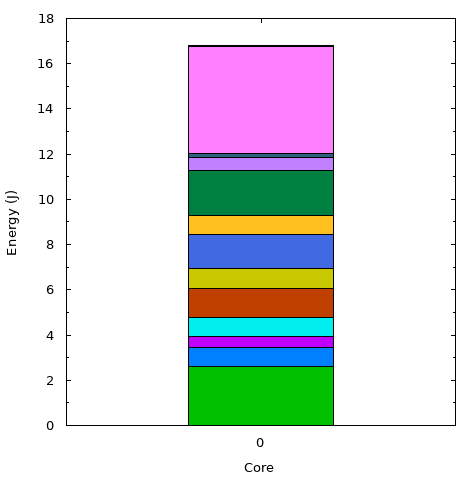
\includegraphics[width=1\textwidth]{output/npb-is/8way-lru/power-chop.png}
                    \caption{L3 energy 0.20 J; Total energy 16.79 J}
                    \label{appfig:power:is:lru:8}
                \end{subfigure} &
                \begin{subfigure}{0.42\textwidth}
                    \centering
                    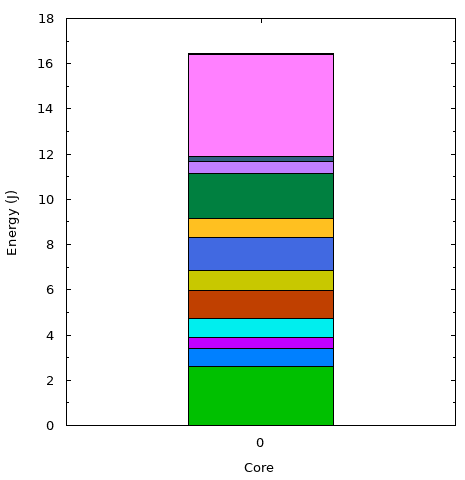
\includegraphics[width=1\textwidth]{output/npb-is/16way-lru/power-chop.png}
                    \caption{L3 energy 0.21 J; Total energy 16.43 J}
                    \label{appfig:power:is:lru:16}
                \end{subfigure} &
                \begin{subfigure}{0.42\textwidth}
                    \centering
                    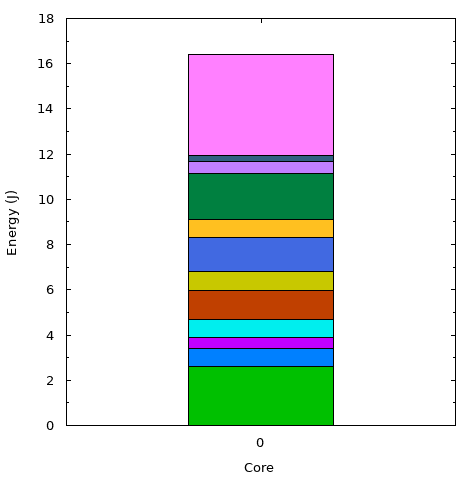
\includegraphics[width=1\textwidth]{output/npb-is/32way-lru/power-chop.png}
                    \caption{L3 energy 0.27 J; Total energy 16.40 J}
                    \label{appfig:power:is:lru:32}
                \end{subfigure} 
            \end{tabular}
            \end{adjustwidth}
            \caption{Processor power with an (\ref{appfig:power:is:lru:8}) 8-way, (\ref{appfig:power:is:lru:16}) 16-way, and (\ref{appfig:power:is:lru:32}) 32-way L3 cache using LRU replacement policy.}
            \label{appfig:power:is:lru}
        \end{figure}

        % SRRIP
        \begin{figure}[hbt!]
            \centering 
            \begin{adjustwidth}{-2.75cm}{}
            \begin{tabular}{ccc}
                \begin{subfigure}{0.42\textwidth}
                    \centering
                    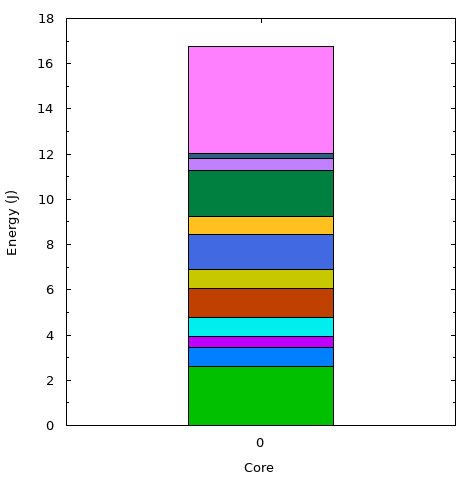
\includegraphics[width=1\textwidth]{output/npb-is/8way-srrip/power-chop.png}
                    \caption{L3 energy 0.20 J; Total energy 16.75 J}
                    \label{appfig:power:is:srrip:8}
                \end{subfigure} &
                \begin{subfigure}{0.42\textwidth}
                    \centering
                    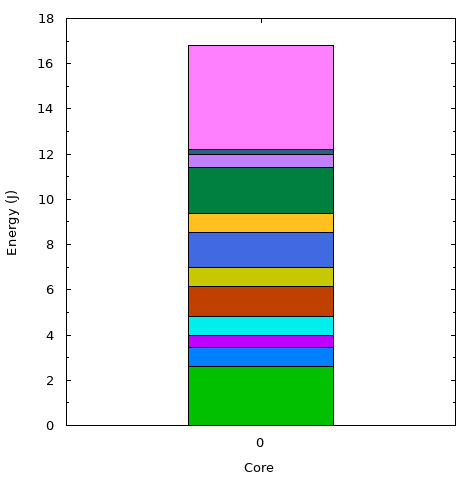
\includegraphics[width=1\textwidth]{output/npb-is/16way-srrip/power-chop.png}
                    \caption{L3 energy 0.22 J; Total energy 16.82 J}
                    \label{appfig:power:is:srrip:16}
                \end{subfigure} &
                \begin{subfigure}{0.42\textwidth}
                    \centering
                    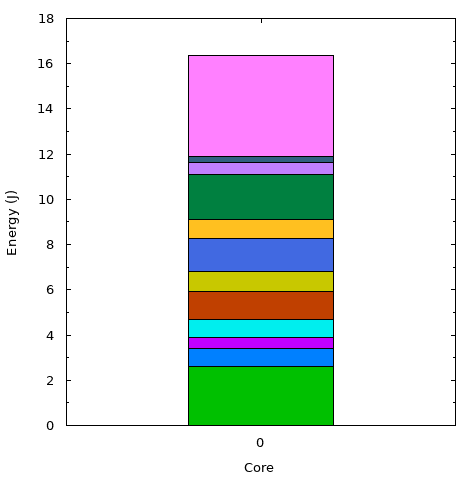
\includegraphics[width=1\textwidth]{output/npb-is/32way-srrip/power-chop.png}
                    \caption{L3 energy 0.27 J; Total energy 16.35 J}
                    \label{appfig:power:is:srrip:32}
                \end{subfigure} 
            \end{tabular}
            \end{adjustwidth}
            \caption{Processor power with an (\ref{appfig:power:is:srrip:8}) 8-way, (\ref{appfig:power:is:srrip:16}) 16-way, and (\ref{appfig:power:is:srrip:32}) 32-way L3 cache using SRRIP replacement policy.}
            \label{appfig:power:is:srrip}
        \end{figure}

        % RR
        \begin{figure}[hbt!]
            \centering 
            \begin{adjustwidth}{-2.75cm}{}
            \begin{tabular}{ccc}
                \begin{subfigure}{0.42\textwidth}
                    \centering
                    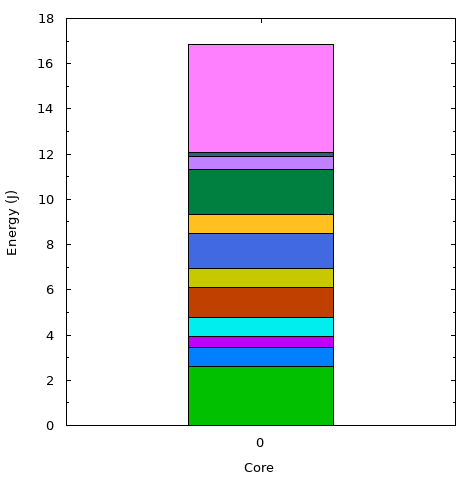
\includegraphics[width=1\textwidth]{output/npb-is/8way-rr/power-chop.png}
                    \caption{L3 energy 0.20 J; Total energy 16.87 J}
                    \label{appfig:power:is:rr:8}
                \end{subfigure} &
                \begin{subfigure}{0.42\textwidth}
                    \centering
                    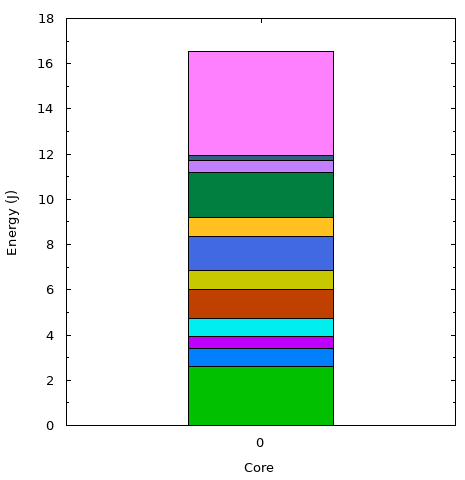
\includegraphics[width=1\textwidth]{output/npb-is/16way-rr/power-chop.png}
                    \caption{L3 energy 0.21 J; Total energy 16.56 J}
                    \label{appfig:power:is:rr:16}
                \end{subfigure} &
                \begin{subfigure}{0.42\textwidth}
                    \centering
                    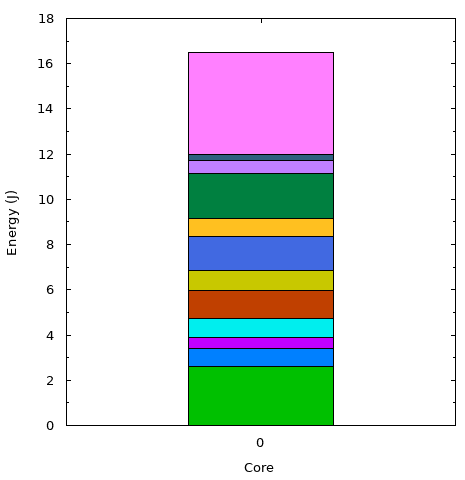
\includegraphics[width=1\textwidth]{output/npb-is/32way-rr/power-chop.png}
                    \caption{L3 energy 0.27 J; Total energy 16.51 J}
                    \label{appfig:power:is:rr:32}
                \end{subfigure} 
            \end{tabular}
            \end{adjustwidth}
            \caption{Processor power with an (\ref{appfig:power:is:rr:8}) 8-way, (\ref{appfig:power:is:rr:16}) 16-way, and (\ref{appfig:power:is:rr:32}) 32-way L3 cache using round robin replacement policy.}
            \label{appfig:power:is:rr}
        \end{figure}

        % legend
        \begin{figure}
            \centering 
            \begin{adjustwidth}{-2.75cm}{}
            \begin{tabular}{ccc}
                & & 
                \begin{subfigure}{0.33\textwidth}
                    \centering
                    \includegraphics[width=1\textwidth]{output/npb-is/8way-lru/power-legend.png}
                    % \caption{}
                    \label{appfig:power:is:legend}
                \end{subfigure} 
            \end{tabular}
        \end{adjustwidth}
        \end{figure}
        \clearpage

        \begin{figure}[hbt!]
            \centering
            \noindent\begin{subfigure}{0.75\textwidth}
            \lstinputlisting{output/npb-is/8way-lru/power.out}
            \caption{}
            \end{subfigure}%

            \noindent\begin{subfigure}{0.75\textwidth}
            \lstinputlisting{output/npb-is/16way-lru/power.out}
            \caption{}
            \end{subfigure}%
        \end{figure}
        \clearpage

        \begin{figure}[hbt!]\ContinuedFloat
            \centering
            \noindent\begin{subfigure}{0.75\textwidth}
            \lstinputlisting{output/npb-is/32way-lru/power.out}
            \caption{}
            \end{subfigure}%
            \caption{Specific values for each components' power consumption (See. Fig. \ref{appfig:power:is:lru}), for \texttt{npb-is} benchmark with (LRU) L3 associativity of (a) 8, (b) 16, and (c) 32 way.}
            \label{appfig:power:is:lru:values}
        \end{figure}
        \clearpage

        \begin{figure}[hbt!]
            \centering
            \noindent\begin{subfigure}{0.75\textwidth}
            \lstinputlisting{output/npb-is/8way-srrip/power.out}
            \caption{}
            \end{subfigure}%

            \noindent\begin{subfigure}{0.75\textwidth}
            \lstinputlisting{output/npb-is/16way-srrip/power.out}
            \caption{}
            \end{subfigure}%
        \end{figure}
        \clearpage

        \begin{figure}[hbt!]\ContinuedFloat
            \centering
            \noindent\begin{subfigure}{0.75\textwidth}
            \lstinputlisting{output/npb-is/32way-srrip/power.out}
            \caption{}
            \end{subfigure}%
            \caption{Specific values for each components' power consumption (See. Fig. \ref{appfig:power:is:srrip}), for \texttt{npb-is} benchmark with (SRRIP) L3 associativity of (a) 8, (b) 16, and (c) 32 way.}
            \label{appfig:power:is:srrip:values}
        \end{figure}
        \clearpage

        \begin{figure}[hbt!]
            \centering
            \noindent\begin{subfigure}{0.75\textwidth}
            \lstinputlisting{output/npb-is/8way-rr/power.out}
            \caption{}
            \end{subfigure}%

            \noindent\begin{subfigure}{0.75\textwidth}
            \lstinputlisting{output/npb-is/16way-rr/power.out}
            \caption{}
            \end{subfigure}%
        \end{figure}
        \clearpage

        \begin{figure}[hbt!]\ContinuedFloat
            \centering
            \noindent\begin{subfigure}{0.75\textwidth}
            \lstinputlisting{output/npb-is/32way-rr/power.out}
            \caption{}
            \end{subfigure}%
            \caption{Specific values for each components' power consumption (See. Fig. \ref{appfig:power:is:rr}), for \texttt{npb-is} benchmark with (round robin) L3 associativity of (a) 8, (b) 16, and (c) 32 way.}
            \label{appfig:power:is:rr:values}
        \end{figure}
        \clearpage


        %%%%%%%%%%%%%%%%%%%%%%%%%%%%%%%%%%%%%%%%%%%%%%%%%%%%%%%%%%%%%%%%%%%%%%

        \subsubsection{CPI Stacks} %%%%%%%%%%%%%%%%%%%%%%%%%%%%%%%%%%%
        % LRU
        \begin{figure}[hbt!]
            \centering 
            \begin{adjustwidth}{-2.75cm}{}
            \begin{tabular}{ccc}
                \begin{subfigure}{0.42\textwidth}
                    \centering
                    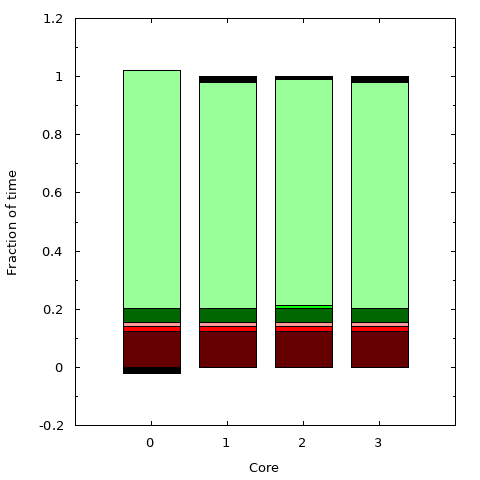
\includegraphics[width=1\textwidth]{output/npb-is/8way-lru/cpi-stack-chop.png}
                    \caption{}
                    \label{appfig:cpi:is:lru:8}
                \end{subfigure} &
                \begin{subfigure}{0.42\textwidth}
                    \centering
                    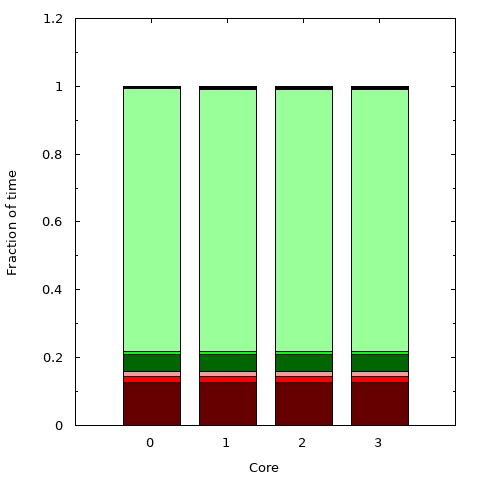
\includegraphics[width=1\textwidth]{output/npb-is/16way-lru/cpi-stack-chop.png}
                    \caption{}
                    \label{appfig:cpi:is:lru:16}
                \end{subfigure} &
                \begin{subfigure}{0.42\textwidth}
                    \centering
                    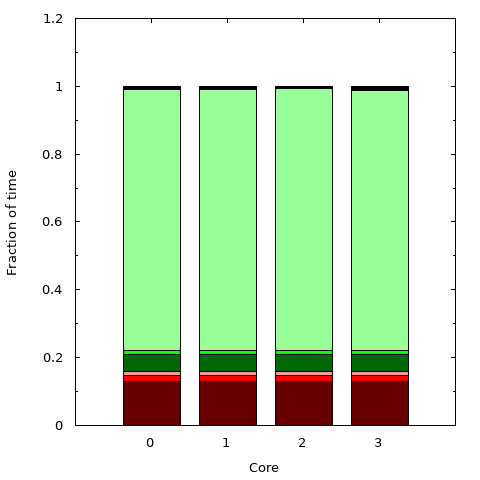
\includegraphics[width=1\textwidth]{output/npb-is/32way-lru/cpi-stack-chop.png}
                    \caption{}
                    \label{appfig:cpi:is:lru:32}
                \end{subfigure} 
            \end{tabular}
            \end{adjustwidth}
            \caption{CPI stack with an (\ref{appfig:cpi:is:lru:8}) 8-way, (\ref{appfig:cpi:is:lru:16}) 16-way, and (\ref{appfig:cpi:is:lru:32}) 32-way L3 cache using LRU replacement policy.}
            \label{appfig:cpi:is:lru}
        \end{figure}

        % SRRIP
        \begin{figure}[hbt!]
            \centering 
            \begin{adjustwidth}{-2.75cm}{}
            \begin{tabular}{ccc}
                \begin{subfigure}{0.42\textwidth}
                    \centering
                    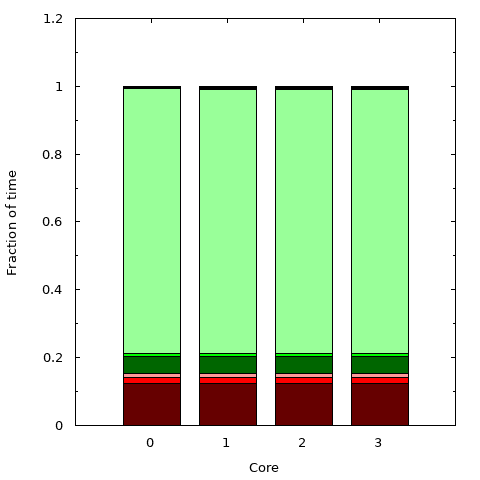
\includegraphics[width=1\textwidth]{output/npb-is/8way-srrip/cpi-stack-chop.png}
                    \caption{}
                    \label{appfig:cpi:is:srrip:8}
                \end{subfigure} &
                \begin{subfigure}{0.42\textwidth}
                    \centering
                    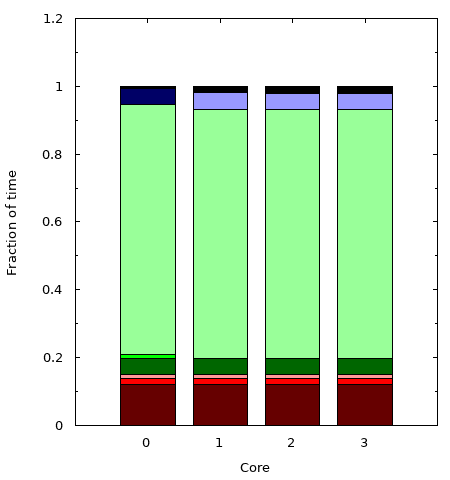
\includegraphics[width=.95\textwidth]{output/npb-is/16way-srrip/cpi-stack-chop.png}
                    \caption{}
                    \label{appfig:cpi:is:srrip:16}
                \end{subfigure} &
                \begin{subfigure}{0.42\textwidth}
                    \centering
                    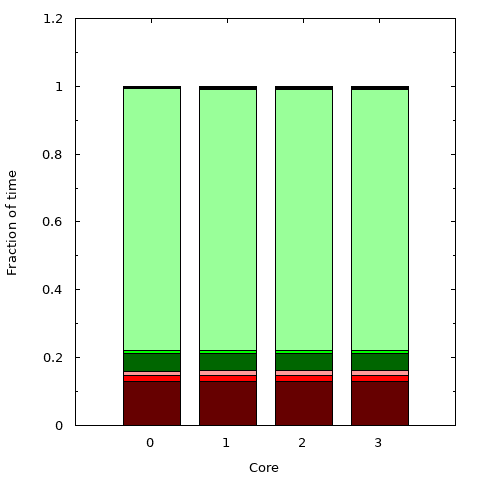
\includegraphics[width=1\textwidth]{output/npb-is/32way-srrip/cpi-stack-chop.png}
                    \caption{}
                    \label{appfig:cpi:is:srrip:32}
                \end{subfigure} 
            \end{tabular}
            \end{adjustwidth}
            \caption{CPI stack with an (\ref{appfig:cpi:is:srrip:8}) 8-way, (\ref{appfig:cpi:is:srrip:16}) 16-way, and (\ref{appfig:cpi:is:srrip:32}) 32-way L3 cache using SRRIP replacement policy.}
            \label{appfig:cpi:is:srrip}
        \end{figure}


        % RR
        \begin{figure}[hbt!]
            \centering 
            \begin{adjustwidth}{-2.75cm}{}
            \begin{tabular}{ccc}
                \begin{subfigure}{0.42\textwidth}
                    \centering
                    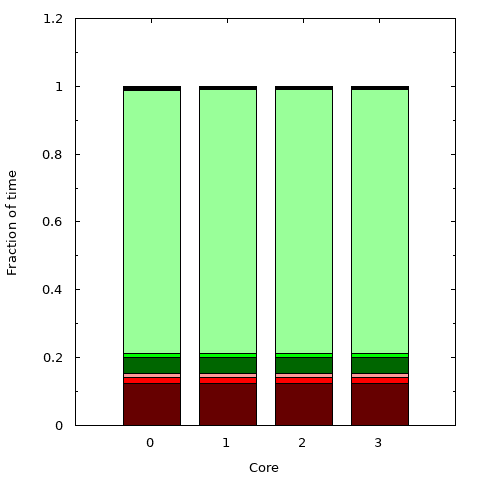
\includegraphics[width=1\textwidth]{output/npb-is/8way-rr/cpi-stack-chop.png}
                    \caption{}
                    \label{appfig:cpi:is:rr:8}
                \end{subfigure} &
                \begin{subfigure}{0.42\textwidth}
                    \centering
                    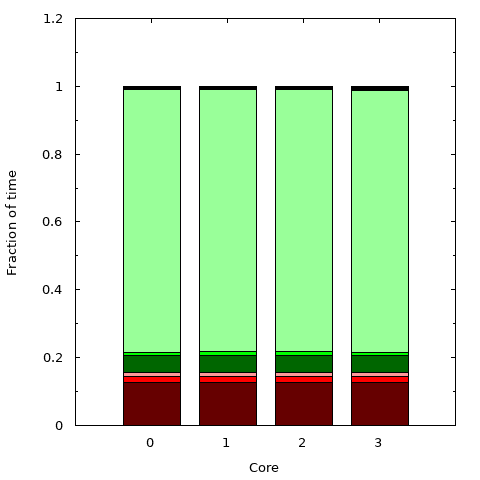
\includegraphics[width=.95\textwidth]{output/npb-is/16way-rr/cpi-stack-chop.png}
                    \caption{}
                    \label{appfig:cpi:is:rr:16}
                \end{subfigure} &
                \begin{subfigure}{0.42\textwidth}
                    \centering
                    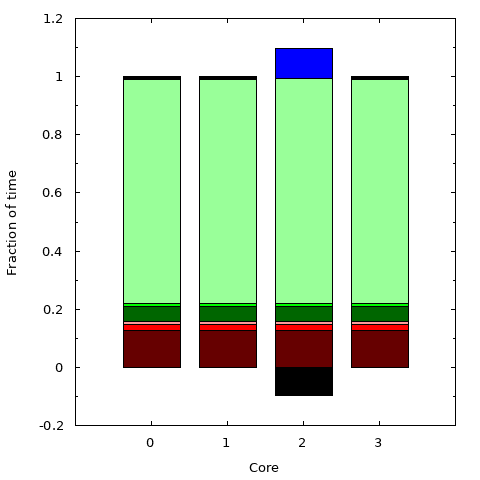
\includegraphics[width=1\textwidth]{output/npb-is/32way-rr/cpi-stack-chop.png}
                    \caption{}
                    \label{appfig:cpi:is:rr:32}
                \end{subfigure} 
            \end{tabular}
            \end{adjustwidth}
            \caption{CPI stack with an (\ref{appfig:cpi:is:rr:8}) 8-way, (\ref{appfig:cpi:is:rr:16}) 16-way, and (\ref{appfig:cpi:is:rr:32}) 32-way L3 cache using round robin replacement policy.}
            \label{appfig:cpi:is:rr}
        \end{figure}

        % legend
        \begin{figure}
            \centering 
            \begin{adjustwidth}{-2.75cm}{}
            \begin{tabular}{ccc}
                & 
                \begin{subfigure}{0.33\textwidth}
                    \centering
                    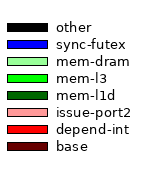
\includegraphics[width=1\textwidth]{output/npb-is/32way-rr/cpi-stack-legend.png}
                    % \caption{}
                    \label{appfig:cpi:is:legend1}
                \end{subfigure} 
                & 
                \begin{subfigure}{0.33\textwidth}
                    \centering
                    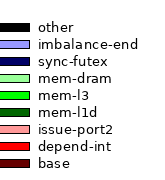
\includegraphics[width=1\textwidth]{output/npb-is/16way-srrip/cpi-stack-legend.png}
                    % \caption{}
                    \label{appfig:cpi:is:legend2}
                \end{subfigure} 
            \end{tabular}
        \end{adjustwidth}
        \end{figure}

        \begin{figure}[hbt!]
            \centering
            \noindent\begin{subfigure}{0.75\textwidth}
            \lstinputlisting{output/npb-is/8way-lru/cpi-stack.out}
            \caption{}
            \end{subfigure}%

            \noindent\begin{subfigure}{0.75\textwidth}
            \lstinputlisting{output/npb-is/16way-lru/cpi-stack.out}
            \caption{}
            \end{subfigure}%
        % \end{figure}
        % \clearpage

        % \begin{figure}[hbt!]\ContinuedFloat
        %     \centering
            \noindent\begin{subfigure}{0.75\textwidth}
            \lstinputlisting{output/npb-is/32way-lru/cpi-stack.out}
            \caption{}
            \end{subfigure}%
            \caption{Specific values for each components' CPI stack fraction of time (See. Fig. \ref{appfig:cpi:is:lru}), for \texttt{npb-is} benchmark with (LRU) L3 associativity of (a) 8, (b) 16, and (c) 32 way.}
            \label{appfig:cpi:is:lru:values}
        \end{figure}
        \clearpage

        \begin{figure}[hbt!]
            \centering
            \noindent\begin{subfigure}{0.75\textwidth}
            \lstinputlisting{output/npb-is/8way-srrip/cpi-stack.out}
            \caption{}
            \end{subfigure}%

            \noindent\begin{subfigure}{0.75\textwidth}
            \lstinputlisting{output/npb-is/16way-srrip/cpi-stack.out}
            \caption{}
            \end{subfigure}%
        % \end{figure}
        % \clearpage

        % \begin{figure}[hbt!]\ContinuedFloat
        %     \centering
            \noindent\begin{subfigure}{0.75\textwidth}
            \lstinputlisting{output/npb-is/32way-srrip/cpi-stack.out}
            \caption{}
            \end{subfigure}%
            \caption{Specific values for each components' CPI stack fraction of time (See. Fig. \ref{appfig:cpi:is:srrip}), for \texttt{npb-is} benchmark with (SRRIP) L3 associativity of (a) 8, (b) 16, and (c) 32 way.}
            \label{appfig:cpi:is:srrip:values}
        \end{figure}
        \clearpage

        \begin{figure}[hbt!]
            \centering
            \noindent\begin{subfigure}{0.75\textwidth}
            \lstinputlisting{output/npb-is/8way-rr/cpi-stack.out}
            \caption{}
            \end{subfigure}%

            \noindent\begin{subfigure}{0.75\textwidth}
            \lstinputlisting{output/npb-is/16way-rr/cpi-stack.out}
            \caption{}
            \end{subfigure}%
        % \end{figure}
        % \clearpage

        % \begin{figure}[hbt!]\ContinuedFloat
        %     \centering
            \noindent\begin{subfigure}{0.75\textwidth}
            \lstinputlisting{output/npb-is/32way-rr/cpi-stack.out}
            \caption{}
            \end{subfigure}%
            \caption{Specific values for each components' CPI stack fraction of time (See. Fig. \ref{appfig:cpi:is:rr}), for \texttt{npb-is} benchmark with (round robin) L3 associativity of (a) 8, (b) 16, and (c) 32 way.}
            \label{appfig:cpi:is:rr:values}
        \end{figure}
        \clearpage

   %%%%%%%%%%%%%%%%%%%%%%%%%%%%%%%%%%%%%%%%%%%%%%%%%%%%%%%%%%%%%%%%%%%%%%


   \subsection{splash2-ocean.cont} %%%%%%%%%%%%%%%%%%%%%%%%%%%%%%%%%%%
        
        \subsubsection{Power Results} %%%%%%%%%%%%%%%%%%%%%%%%%%%%%%%%%%%

        % LRU
        \begin{figure}[hbt!]
            \centering 
            \begin{adjustwidth}{-2.75cm}{}
            \begin{tabular}{ccc}
                \begin{subfigure}{0.42\textwidth}
                    \centering
                    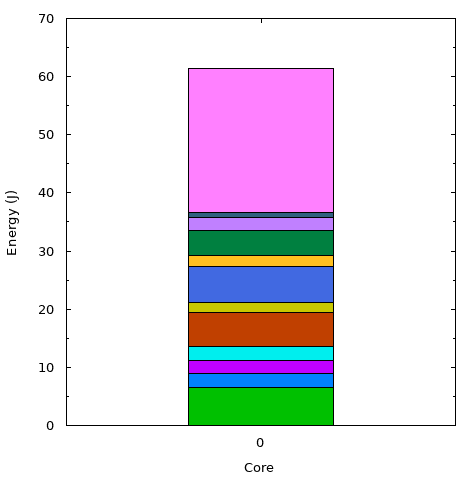
\includegraphics[width=1\textwidth]{output/splash2-ocean.cont/8way-lru/power-chop.png}
                    \caption{L3 energy 0.86 J; Total energy 61.46 J}
                    \label{appfig:power:ocean:lru:8}
                \end{subfigure} &
                \begin{subfigure}{0.42\textwidth}
                    \centering
                    \includegraphics[width=1\textwidth]{output/splash2-ocean.cont/16way-lru/power-chop.png}
                    \caption{L3 energy 0.92 J; Total energy 61.40 J}
                    \label{appfig:power:ocean:lru:16}
                \end{subfigure} &
                \begin{subfigure}{0.42\textwidth}
                    \centering
                    \includegraphics[width=1\textwidth]{output/splash2-ocean.cont/32way-lru/power-chop.png}
                    \caption{L3 energy 1.18 J; Total energy 61.74 J}
                    \label{appfig:power:ocean:lru:32}
                \end{subfigure} 
            \end{tabular}
            \end{adjustwidth}
            \caption{Processor power with an (\ref{appfig:power:ocean:lru:8}) 8-way, (\ref{appfig:power:ocean:lru:16}) 16-way, and (\ref{appfig:power:ocean:lru:32}) 32-way L3 cache using LRU replacement policy.}
            \label{appfig:power:ocean:lru}
        \end{figure}

        % SRRIP
        \begin{figure}[hbt!]
            \centering 
            \begin{adjustwidth}{-2.75cm}{}
            \begin{tabular}{ccc}
                \begin{subfigure}{0.42\textwidth}
                    \centering
                    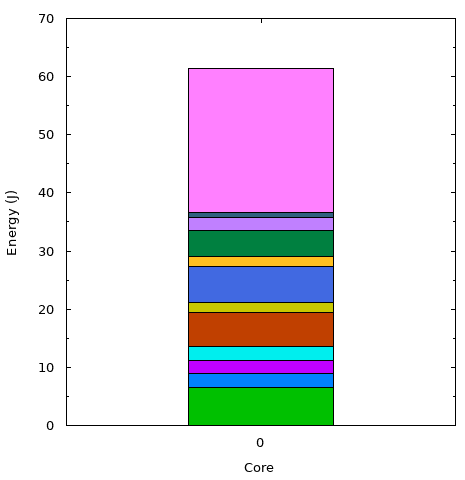
\includegraphics[width=1\textwidth]{output/splash2-ocean.cont/8way-srrip/power-chop.png}
                    \caption{L3 energy 0.86 J; Total energy 61.39 J}
                    \label{appfig:power:ocean:srrip:8}
                \end{subfigure} &
                \begin{subfigure}{0.42\textwidth}
                    \centering
                    \includegraphics[width=1\textwidth]{output/splash2-ocean.cont/16way-srrip/power-chop.png}
                    \caption{L3 energy 0.92 J; Total energy 61.41 J}
                    \label{appfig:power:ocean:srrip:16}
                \end{subfigure} &
                \begin{subfigure}{0.42\textwidth}
                    \centering
                    \includegraphics[width=1\textwidth]{output/splash2-ocean.cont/32way-srrip/power-chop.png}
                    \caption{L3 energy 1.18 J; Total energy 61.72}
                    \label{appfig:power:ocean:srrip:32}
                \end{subfigure} 
            \end{tabular}
            \end{adjustwidth}
            \caption{Processor power with an (\ref{appfig:power:ocean:srrip:8}) 8-way, (\ref{appfig:power:ocean:srrip:16}) 16-way, and (\ref{appfig:power:ocean:srrip:32}) 32-way L3 cache using SRRIP replacement policy.}
            \label{appfig:power:ocean:srrip}
        \end{figure}

        % RR
        \begin{figure}[hbt!]
            \centering 
            \begin{adjustwidth}{-2.75cm}{}
            \begin{tabular}{ccc}
                \begin{subfigure}{0.42\textwidth}
                    \centering
                    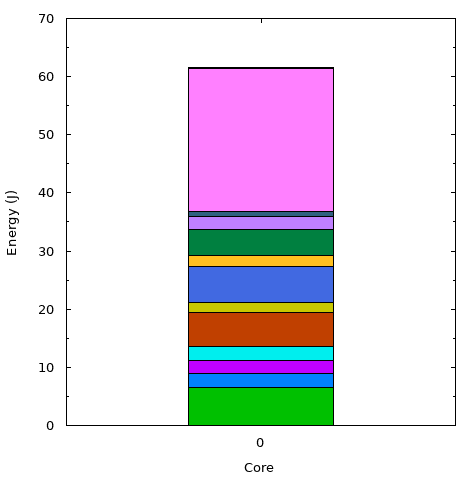
\includegraphics[width=1\textwidth]{output/splash2-ocean.cont/8way-rr/power-chop.png}
                    \caption{L3 energy 0.86 J; Total energy 61.52 J}
                    \label{appfig:power:ocean:rr:8}
                \end{subfigure} &
                \begin{subfigure}{0.42\textwidth}
                    \centering
                    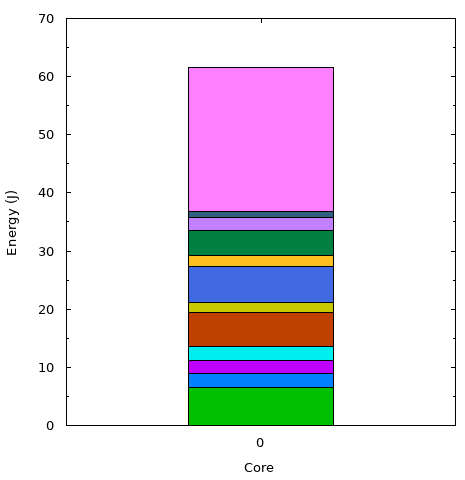
\includegraphics[width=1\textwidth]{output/splash2-ocean.cont/16way-rr/power-chop.png}
                    \caption{L3 energy 0.93 J; Total energy 61.54 J}
                    \label{appfig:power:ocean:rr:16}
                \end{subfigure} &
                \begin{subfigure}{0.42\textwidth}
                    \centering
                    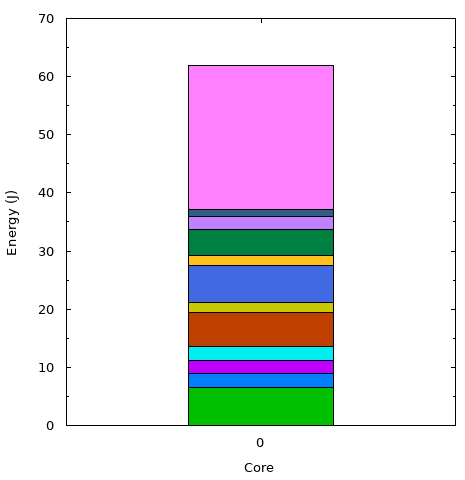
\includegraphics[width=1\textwidth]{output/splash2-ocean.cont/32way-rr/power-chop.png}
                    \caption{L3 energy 1.19 J; Total energy 61.91 J}
                    \label{appfig:power:ocean:rr:32}
                \end{subfigure} 
            \end{tabular}
            \end{adjustwidth}
            \caption{Processor power with an (\ref{appfig:power:ocean:rr:8}) 8-way, (\ref{appfig:power:ocean:rr:16}) 16-way, and (\ref{appfig:power:ocean:rr:32}) 32-way L3 cache using round robin replacement policy.}
            \label{appfig:power:ocean:rr}
        \end{figure}

        % legend
        \begin{figure}
            \centering 
            \begin{adjustwidth}{-2.75cm}{}
            \begin{tabular}{ccc}
                & & 
                \begin{subfigure}{0.33\textwidth}
                    \centering
                    \includegraphics[width=1\textwidth]{output/splash2-ocean.cont/8way-lru/power-legend.png}
                    % \caption{}
                    \label{appfig:power:ocean:legend}
                \end{subfigure} 
            \end{tabular}
        \end{adjustwidth}
        \end{figure}
        \clearpage

        \begin{figure}[hbt!]
            \centering
            \noindent\begin{subfigure}{0.75\textwidth}
            \lstinputlisting{output/splash2-ocean.cont/8way-lru/power.out}
            \caption{}
            \end{subfigure}%

            \noindent\begin{subfigure}{0.75\textwidth}
            \lstinputlisting{output/splash2-ocean.cont/16way-lru/power.out}
            \caption{}
            \end{subfigure}%
        \end{figure}
        \clearpage

        \begin{figure}[hbt!]\ContinuedFloat
            \centering
            \noindent\begin{subfigure}{0.75\textwidth}
            \lstinputlisting{output/splash2-ocean.cont/32way-lru/power.out}
            \caption{}
            \end{subfigure}%
            \caption{Specific values for each components' power consumption (See. Fig. \ref{appfig:power:ocean:lru}), for \texttt{splash2-ocean.cont} benchmark with (LRU) L3 associativity of (a) 8, (b) 16, and (c) 32 way.}
            \label{appfig:power:ocean:lru:values}
        \end{figure}
        \clearpage

        \begin{figure}[hbt!]
            \centering
            \noindent\begin{subfigure}{0.75\textwidth}
            \lstinputlisting{output/splash2-ocean.cont/8way-srrip/power.out}
            \caption{}
            \end{subfigure}%

            \noindent\begin{subfigure}{0.75\textwidth}
            \lstinputlisting{output/splash2-ocean.cont/16way-srrip/power.out}
            \caption{}
            \end{subfigure}%
        \end{figure}
        \clearpage

        \begin{figure}[hbt!]\ContinuedFloat
            \centering
            \noindent\begin{subfigure}{0.75\textwidth}
            \lstinputlisting{output/splash2-ocean.cont/32way-srrip/power.out}
            \caption{}
            \end{subfigure}%
            \caption{Specific values for each components' power consumption (See. Fig. \ref{appfig:power:ocean:srrip}), for \texttt{splash2-ocean.cont} benchmark with (SRRIP) L3 associativity of (a) 8, (b) 16, and (c) 32 way.}
            \label{appfig:power:ocean:srrip:values}
        \end{figure}
        \clearpage

        \begin{figure}[hbt!]
            \centering
            \noindent\begin{subfigure}{0.75\textwidth}
            \lstinputlisting{output/splash2-ocean.cont/8way-rr/power.out}
            \caption{}
            \end{subfigure}%

            \noindent\begin{subfigure}{0.75\textwidth}
            \lstinputlisting{output/splash2-ocean.cont/16way-rr/power.out}
            \caption{}
            \end{subfigure}%
        \end{figure}
        \clearpage

        \begin{figure}[hbt!]\ContinuedFloat
            \centering
            \noindent\begin{subfigure}{0.75\textwidth}
            \lstinputlisting{output/splash2-ocean.cont/32way-rr/power.out}
            \caption{}
            \end{subfigure}%
            \caption{Specific values for each components' power consumption (See. Fig. \ref{appfig:power:ocean:rr}), for \texttt{splash2-ocean.cont} benchmark with (round robin) L3 associativity of (a) 8, (b) 16, and (c) 32 way.}
            \label{appfig:power:ocean:rr:values}
        \end{figure}
        \clearpage


        %%%%%%%%%%%%%%%%%%%%%%%%%%%%%%%%%%%%%%%%%%%%%%%%%%%%%%%%%%%%%%%%%%%%%%

        \subsubsection{CPI Stacks} %%%%%%%%%%%%%%%%%%%%%%%%%%%%%%%%%%%
        % LRU
        \begin{figure}[hbt!]
            \centering 
            \begin{adjustwidth}{-2.75cm}{}
            \begin{tabular}{ccc}
                \begin{subfigure}{0.42\textwidth}
                    \centering
                    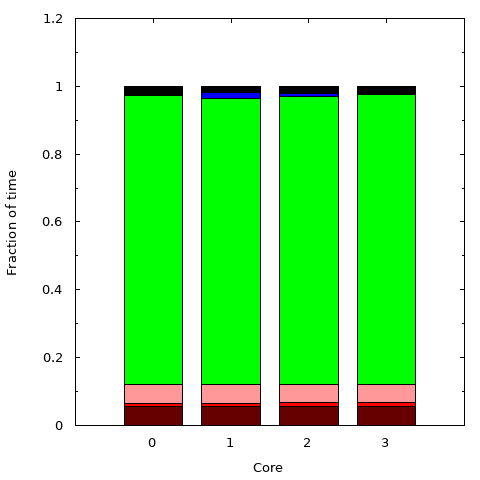
\includegraphics[width=1\textwidth]{output/splash2-ocean.cont/8way-lru/cpi-stack-chop.png}
                    \caption{}
                    \label{appfig:cpi:ocean:lru:8}
                \end{subfigure} &
                \begin{subfigure}{0.42\textwidth}
                    \centering
                    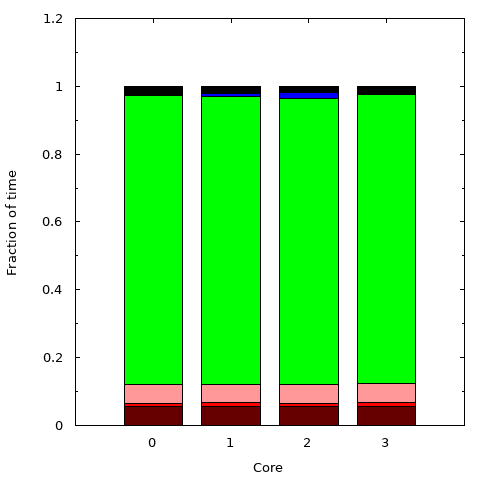
\includegraphics[width=1\textwidth]{output/splash2-ocean.cont/16way-lru/cpi-stack-chop.png}
                    \caption{}
                    \label{appfig:cpi:ocean:lru:16}
                \end{subfigure} &
                \begin{subfigure}{0.42\textwidth}
                    \centering
                    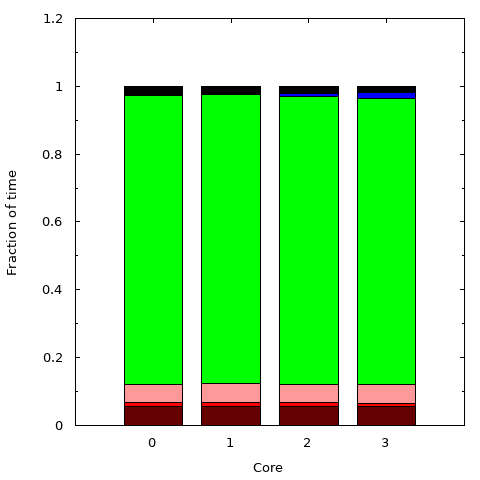
\includegraphics[width=1\textwidth]{output/splash2-ocean.cont/32way-lru/cpi-stack-chop.png}
                    \caption{}
                    \label{appfig:cpi:ocean:lru:32}
                \end{subfigure} 
            \end{tabular}
            \end{adjustwidth}
            \caption{CPI stack with an (\ref{appfig:cpi:ocean:lru:8}) 8-way, (\ref{appfig:cpi:ocean:lru:16}) 16-way, and (\ref{appfig:cpi:ocean:lru:32}) 32-way L3 cache using LRU replacement policy.}
            \label{appfig:cpi:ocean:lru}
        \end{figure}

        % SRRIP
        \begin{figure}[hbt!]
            \centering 
            \begin{adjustwidth}{-2.75cm}{}
            \begin{tabular}{ccc}
                \begin{subfigure}{0.42\textwidth}
                    \centering
                    \includegraphics[width=1\textwidth]{output/splash2-ocean.cont/8way-srrip/cpi-stack-chop.png}
                    \caption{}
                    \label{appfig:cpi:ocean:srrip:8}
                \end{subfigure} &
                \begin{subfigure}{0.42\textwidth}
                    \centering
                    \includegraphics[width=.95\textwidth]{output/splash2-ocean.cont/16way-srrip/cpi-stack-chop.png}
                    \caption{}
                    \label{appfig:cpi:ocean:srrip:16}
                \end{subfigure} &
                \begin{subfigure}{0.42\textwidth}
                    \centering
                    \includegraphics[width=1\textwidth]{output/splash2-ocean.cont/32way-srrip/cpi-stack-chop.png}
                    \caption{}
                    \label{appfig:cpi:ocean:srrip:32}
                \end{subfigure} 
            \end{tabular}
            \end{adjustwidth}
            \caption{CPI stack with an (\ref{appfig:cpi:ocean:srrip:8}) 8-way, (\ref{appfig:cpi:ocean:srrip:16}) 16-way, and (\ref{appfig:cpi:ocean:srrip:32}) 32-way L3 cache using SRRIP replacement policy.}
            \label{appfig:cpi:ocean:srrip}
        \end{figure}


        % RR
        \begin{figure}[hbt!]
            \centering 
            \begin{adjustwidth}{-2.75cm}{}
            \begin{tabular}{ccc}
                \begin{subfigure}{0.42\textwidth}
                    \centering
                    \includegraphics[width=1\textwidth]{output/splash2-ocean.cont/8way-rr/cpi-stack-chop.png}
                    \caption{}
                    \label{appfig:cpi:ocean:rr:8}
                \end{subfigure} &
                \begin{subfigure}{0.42\textwidth}
                    \centering
                    \includegraphics[width=.95\textwidth]{output/splash2-ocean.cont/16way-rr/cpi-stack-chop.png}
                    \caption{}
                    \label{appfig:cpi:ocean:rr:16}
                \end{subfigure} &
                \begin{subfigure}{0.42\textwidth}
                    \centering
                    \includegraphics[width=1\textwidth]{output/splash2-ocean.cont/32way-rr/cpi-stack-chop.png}
                    \caption{}
                    \label{appfig:cpi:ocean:rr:32}
                \end{subfigure} 
            \end{tabular}
            \end{adjustwidth}
            \caption{CPI stack with an (\ref{appfig:cpi:ocean:rr:8}) 8-way, (\ref{appfig:cpi:ocean:rr:16}) 16-way, and (\ref{appfig:cpi:ocean:rr:32}) 32-way L3 cache using round robin replacement policy.}
            \label{appfig:cpi:ocean:rr}
        \end{figure}

        % legend
        \begin{figure}
            \centering 
            \begin{adjustwidth}{-2.75cm}{}
            \begin{tabular}{ccc}
                & 
                % \begin{subfigure}{0.33\textwidth}
                %     \centering
                %     \includegraphics[width=1\textwidth]{output/npb-is/32way-rr/cpi-stack-legend.png}
                %     % \caption{}
                %     \label{appfig:cpi:is:legend1}
                % \end{subfigure} 
                & 
                \begin{subfigure}{0.33\textwidth}
                    \centering
                    \includegraphics[width=1\textwidth]{output/splash2-ocean.cont/16way-srrip/cpi-stack-legend.png}
                    % \caption{}
                    \label{appfig:cpi:ocean:legend2}
                \end{subfigure} 
            \end{tabular}
        \end{adjustwidth}
        \end{figure}

        \begin{figure}[hbt!]
            \centering
            \noindent\begin{subfigure}{0.75\textwidth}
            \lstinputlisting{output/splash2-ocean.cont/8way-lru/cpi-stack.out}
            \caption{}
            \end{subfigure}%

            \noindent\begin{subfigure}{0.75\textwidth}
            \lstinputlisting{output/splash2-ocean.cont/16way-lru/cpi-stack.out}
            \caption{}
            \end{subfigure}%
        % \end{figure}
        % \clearpage

        % \begin{figure}[hbt!]\ContinuedFloat
        %     \centering
            \noindent\begin{subfigure}{0.75\textwidth}
            \lstinputlisting{output/splash2-ocean.cont/32way-lru/cpi-stack.out}
            \caption{}
            \end{subfigure}%
            \caption{Specific values for each components' CPI stack fraction of time (See. Fig. \ref{appfig:cpi:ocean:lru}), for \texttt{splash2-ocean.cont} benchmark with (LRU) L3 associativity of (a) 8, (b) 16, and (c) 32 way.}
            \label{appfig:cpi:ocean:lru:values}
        \end{figure}
        \clearpage

        \begin{figure}[hbt!]
            \centering
            \noindent\begin{subfigure}{0.75\textwidth}
            \lstinputlisting{output/splash2-ocean.cont/8way-srrip/cpi-stack.out}
            \caption{}
            \end{subfigure}%

            \noindent\begin{subfigure}{0.75\textwidth}
            \lstinputlisting{output/splash2-ocean.cont/16way-srrip/cpi-stack.out}
            \caption{}
            \end{subfigure}%
        % \end{figure}
        % \clearpage

        % \begin{figure}[hbt!]\ContinuedFloat
        %     \centering
            \noindent\begin{subfigure}{0.75\textwidth}
            \lstinputlisting{output/splash2-ocean.cont/32way-srrip/cpi-stack.out}
            \caption{}
            \end{subfigure}%
            \caption{Specific values for each components' CPI stack fraction of time (See. Fig. \ref{appfig:cpi:ocean:srrip}), for \texttt{splash2-ocean.cont} benchmark with (SRRIP) L3 associativity of (a) 8, (b) 16, and (c) 32 way.}
            \label{appfig:cpi:ocean:srrip:values}
        \end{figure}
        \clearpage

        \begin{figure}[hbt!]
            \centering
            \noindent\begin{subfigure}{0.75\textwidth}
            \lstinputlisting{output/splash2-ocean.cont/8way-rr/cpi-stack.out}
            \caption{}
            \end{subfigure}%

            \noindent\begin{subfigure}{0.75\textwidth}
            \lstinputlisting{output/splash2-ocean.cont/16way-rr/cpi-stack.out}
            \caption{}
            \end{subfigure}%
        % \end{figure}
        % \clearpage

        % \begin{figure}[hbt!]\ContinuedFloat
        %     \centering
            \noindent\begin{subfigure}{0.75\textwidth}
            \lstinputlisting{output/splash2-ocean.cont/32way-rr/cpi-stack.out}
            \caption{}
            \end{subfigure}%
            \caption{Specific values for each components' CPI stack fraction of time (See. Fig. \ref{appfig:cpi:ocean:rr}), for \texttt{splash2-ocean.cont} benchmark with (round robin) L3 associativity of (a) 8, (b) 16, and (c) 32 way.}
            \label{appfig:cpi:ocean:rr:values}
        \end{figure}
        \clearpage

   %%%%%%%%%%%%%%%%%%%%%%%%%%%%%%%%%%%%%%%%%%%%%%%%%%%%%%%%%%%%%%%%%%%%%%


   \subsection{splash2-radix} %%%%%%%%%%%%%%%%%%%%%%%%%%%%%%%%%%%
        
        \subsubsection{Power Results} %%%%%%%%%%%%%%%%%%%%%%%%%%%%%%%%%%%

        % LRU
        \begin{figure}[hbt!]
            \centering 
            \begin{adjustwidth}{-2.75cm}{}
            \begin{tabular}{ccc}
                \begin{subfigure}{0.42\textwidth}
                    \centering
                    \includegraphics[width=1\textwidth]{output/splash2-radix/8way-lru/power-chop.png}
                    \caption{L3 energy 0.02 J; Total energy 1.30 J}
                    \label{appfig:power:radix:lru:8}
                \end{subfigure} &
                \begin{subfigure}{0.42\textwidth}
                    \centering
                    \includegraphics[width=1\textwidth]{output/splash2-radix/16way-lru/power-chop.png}
                    \caption{L3 energy 0.02 J; Total energy 1.29 J}
                    \label{appfig:power:radix:lru:16}
                \end{subfigure} &
                \begin{subfigure}{0.42\textwidth}
                    \centering
                    \includegraphics[width=1\textwidth]{output/splash2-radix/32way-lru/power-chop.png}
                    \caption{L3 energy 0.03 J; Total energy 1.30 J}
                    \label{appfig:power:radix:lru:32}
                \end{subfigure} 
            \end{tabular}
            \end{adjustwidth}
            \caption{Processor power with an (\ref{appfig:power:radix:lru:8}) 8-way, (\ref{appfig:power:radix:lru:16}) 16-way, and (\ref{appfig:power:radix:lru:32}) 32-way L3 cache using LRU replacement policy.}
            \label{appfig:power:radix:lru}
        \end{figure}

        % SRRIP
        \begin{figure}[hbt!]
            \centering 
            \begin{adjustwidth}{-2.75cm}{}
            \begin{tabular}{ccc}
                \begin{subfigure}{0.42\textwidth}
                    \centering
                    \includegraphics[width=1\textwidth]{output/splash2-radix/8way-srrip/power-chop.png}
                    \caption{L3 energy 0.02 J; Total energy 1.30 J}
                    \label{appfig:power:radix:srrip:8}
                \end{subfigure} &
                \begin{subfigure}{0.42\textwidth}
                    \centering
                    \includegraphics[width=1\textwidth]{output/splash2-radix/16way-srrip/power-chop.png}
                    \caption{L3 energy 0.02 J; Total energy 1.30 J}
                    \label{appfig:power:radix:srrip:16}
                \end{subfigure} &
                \begin{subfigure}{0.42\textwidth}
                    \centering
                    \includegraphics[width=1\textwidth]{output/splash2-radix/32way-srrip/power-chop.png}
                    \caption{L3 energy 0.03 J; Total energy 1.31 J}
                    \label{appfig:power:radix:srrip:32}
                \end{subfigure} 
            \end{tabular}
            \end{adjustwidth}
            \caption{Processor power with an (\ref{appfig:power:radix:srrip:8}) 8-way, (\ref{appfig:power:radix:srrip:16}) 16-way, and (\ref{appfig:power:radix:srrip:32}) 32-way L3 cache using SRRIP replacement policy.}
            \label{appfig:power:radix:srrip}
        \end{figure}

        % RR
        \begin{figure}[hbt!]
            \centering 
            \begin{adjustwidth}{-2.75cm}{}
            \begin{tabular}{ccc}
                \begin{subfigure}{0.42\textwidth}
                    \centering
                    \includegraphics[width=1\textwidth]{output/splash2-radix/8way-rr/power-chop.png}
                    \caption{L3 energy 0.02 J; Total energy 1.31 J}
                    \label{appfig:power:radix:rr:8}
                \end{subfigure} &
                \begin{subfigure}{0.42\textwidth}
                    \centering
                    \includegraphics[width=1\textwidth]{output/splash2-radix/16way-rr/power-chop.png}
                    \caption{L3 energy 0.02 J; Total energy 1.30 J}
                    \label{appfig:power:radix:rr:16}
                \end{subfigure} &
                \begin{subfigure}{0.42\textwidth}
                    \centering
                    \includegraphics[width=1\textwidth]{output/splash2-radix/32way-rr/power-chop.png}
                    \caption{L3 energy 0.03 J; Total energy 1.31 J}
                    \label{appfig:power:radix:rr:32}
                \end{subfigure} 
            \end{tabular}
            \end{adjustwidth}
            \caption{Processor power with an (\ref{appfig:power:radix:rr:8}) 8-way, (\ref{appfig:power:radix:rr:16}) 16-way, and (\ref{appfig:power:radix:rr:32}) 32-way L3 cache using round robin replacement policy.}
            \label{appfig:power:radix:rr}
        \end{figure}

        % legend
        \begin{figure}
            \centering 
            \begin{adjustwidth}{-2.75cm}{}
            \begin{tabular}{ccc}
                & & 
                \begin{subfigure}{0.33\textwidth}
                    \centering
                    \includegraphics[width=1\textwidth]{output/splash2-radix/8way-lru/power-legend.png}
                    % \caption{}
                    \label{appfig:power:radix:legend}
                \end{subfigure} 
            \end{tabular}
        \end{adjustwidth}
        \end{figure}
        \clearpage

        \begin{figure}[hbt!]
            \centering
            \noindent\begin{subfigure}{0.75\textwidth}
            \lstinputlisting{output/splash2-radix/8way-lru/power.out}
            \caption{}
            \end{subfigure}%

            \noindent\begin{subfigure}{0.75\textwidth}
            \lstinputlisting{output/splash2-radix/16way-lru/power.out}
            \caption{}
            \end{subfigure}%
        \end{figure}
        \clearpage

        \begin{figure}[hbt!]\ContinuedFloat
            \centering
            \noindent\begin{subfigure}{0.75\textwidth}
            \lstinputlisting{output/splash2-radix/32way-lru/power.out}
            \caption{}
            \end{subfigure}%
            \caption{Specific values for each components' power consumption (See. Fig. \ref{appfig:power:radix:lru}), for \texttt{splash2-radix} benchmark with (LRU) L3 associativity of (a) 8, (b) 16, and (c) 32 way.}
            \label{appfig:power:radix:lru:values}
        \end{figure}
        \clearpage

        \begin{figure}[hbt!]
            \centering
            \noindent\begin{subfigure}{0.75\textwidth}
            \lstinputlisting{output/splash2-radix/8way-srrip/power.out}
            \caption{}
            \end{subfigure}%

            \noindent\begin{subfigure}{0.75\textwidth}
            \lstinputlisting{output/splash2-radix/16way-srrip/power.out}
            \caption{}
            \end{subfigure}%
        \end{figure}
        \clearpage

        \begin{figure}[hbt!]\ContinuedFloat
            \centering
            \noindent\begin{subfigure}{0.75\textwidth}
            \lstinputlisting{output/splash2-radix/32way-srrip/power.out}
            \caption{}
            \end{subfigure}%
            \caption{Specific values for each components' power consumption (See. Fig. \ref{appfig:power:radix:srrip}), for \texttt{splash2-radix.cont} benchmark with (SRRIP) L3 associativity of (a) 8, (b) 16, and (c) 32 way.}
            \label{appfig:power:radix:srrip:values}
        \end{figure}
        \clearpage

        \begin{figure}[hbt!]
            \centering
            \noindent\begin{subfigure}{0.75\textwidth}
            \lstinputlisting{output/splash2-radix/8way-rr/power.out}
            \caption{}
            \end{subfigure}%

            \noindent\begin{subfigure}{0.75\textwidth}
            \lstinputlisting{output/splash2-radix/16way-rr/power.out}
            \caption{}
            \end{subfigure}%
        \end{figure}
        \clearpage

        \begin{figure}[hbt!]\ContinuedFloat
            \centering
            \noindent\begin{subfigure}{0.75\textwidth}
            \lstinputlisting{output/splash2-radix/32way-rr/power.out}
            \caption{}
            \end{subfigure}%
            \caption{Specific values for each components' power consumption (See. Fig. \ref{appfig:power:radix:rr}), for \texttt{splash2-radix} benchmark with (round robin) L3 associativity of (a) 8, (b) 16, and (c) 32 way.}
            \label{appfig:power:radix:rr:values}
        \end{figure}
        \clearpage


        %%%%%%%%%%%%%%%%%%%%%%%%%%%%%%%%%%%%%%%%%%%%%%%%%%%%%%%%%%%%%%%%%%%%%%

        \subsubsection{CPI Stacks} %%%%%%%%%%%%%%%%%%%%%%%%%%%%%%%%%%%
        % LRU
        \begin{figure}[hbt!]
            \centering 
            \begin{adjustwidth}{-2.75cm}{}
            \begin{tabular}{ccc}
                \begin{subfigure}{0.42\textwidth}
                    \centering
                    \includegraphics[width=1\textwidth]{output/splash2-radix/8way-lru/cpi-stack-chop.png}
                    \caption{}
                    \label{appfig:cpi:radix:lru:8}
                \end{subfigure} &
                \begin{subfigure}{0.42\textwidth}
                    \centering
                    \includegraphics[width=1\textwidth]{output/splash2-radix/16way-lru/cpi-stack-chop.png}
                    \caption{}
                    \label{appfig:cpi:radix:lru:16}
                \end{subfigure} &
                \begin{subfigure}{0.42\textwidth}
                    \centering
                    \includegraphics[width=1\textwidth]{output/splash2-radix/32way-lru/cpi-stack-chop.png}
                    \caption{}
                    \label{appfig:cpi:radix:lru:32}
                \end{subfigure} 
            \end{tabular}
            \end{adjustwidth}
            \caption{CPI stack with an (\ref{appfig:cpi:radix:lru:8}) 8-way, (\ref{appfig:cpi:radix:lru:16}) 16-way, and (\ref{appfig:cpi:radix:lru:32}) 32-way L3 cache using LRU replacement policy.}
            \label{appfig:cpi:radix:lru}
        \end{figure}

        % SRRIP
        \begin{figure}[hbt!]
            \centering 
            \begin{adjustwidth}{-2.75cm}{}
            \begin{tabular}{ccc}
                \begin{subfigure}{0.42\textwidth}
                    \centering
                    \includegraphics[width=1\textwidth]{output/splash2-radix/8way-srrip/cpi-stack-chop.png}
                    \caption{}
                    \label{appfig:cpi:radix:srrip:8}
                \end{subfigure} &
                \begin{subfigure}{0.42\textwidth}
                    \centering
                    \includegraphics[width=.95\textwidth]{output/splash2-radix/16way-srrip/cpi-stack-chop.png}
                    \caption{}
                    \label{appfig:cpi:radix:srrip:16}
                \end{subfigure} &
                \begin{subfigure}{0.42\textwidth}
                    \centering
                    \includegraphics[width=1\textwidth]{output/splash2-radix/32way-srrip/cpi-stack-chop.png}
                    \caption{}
                    \label{appfig:cpi:radix:srrip:32}
                \end{subfigure} 
            \end{tabular}
            \end{adjustwidth}
            \caption{CPI stack with an (\ref{appfig:cpi:radix:srrip:8}) 8-way, (\ref{appfig:cpi:radix:srrip:16}) 16-way, and (\ref{appfig:cpi:radix:srrip:32}) 32-way L3 cache using SRRIP replacement policy.}
            \label{appfig:cpi:radix:srrip}
        \end{figure}


        % RR
        \begin{figure}[hbt!]
            \centering 
            \begin{adjustwidth}{-2.75cm}{}
            \begin{tabular}{ccc}
                \begin{subfigure}{0.42\textwidth}
                    \centering
                    \includegraphics[width=1\textwidth]{output/splash2-radix/8way-rr/cpi-stack-chop.png}
                    \caption{}
                    \label{appfig:cpi:radix:rr:8}
                \end{subfigure} &
                \begin{subfigure}{0.42\textwidth}
                    \centering
                    \includegraphics[width=.95\textwidth]{output/splash2-radix/16way-rr/cpi-stack-chop.png}
                    \caption{}
                    \label{appfig:cpi:radix:rr:16}
                \end{subfigure} &
                \begin{subfigure}{0.42\textwidth}
                    \centering
                    \includegraphics[width=1\textwidth]{output/splash2-radix/32way-rr/cpi-stack-chop.png}
                    \caption{}
                    \label{appfig:cpi:radix:rr:32}
                \end{subfigure} 
            \end{tabular}
            \end{adjustwidth}
            \caption{CPI stack with an (\ref{appfig:cpi:radix:rr:8}) 8-way, (\ref{appfig:cpi:radix:rr:16}) 16-way, and (\ref{appfig:cpi:radix:rr:32}) 32-way L3 cache using round robin replacement policy.}
            \label{appfig:cpi:radix:rr}
        \end{figure}

        % legend
        \begin{figure}
            \centering 
            \begin{adjustwidth}{-2.75cm}{}
            \begin{tabular}{ccc}
                & 
                % \begin{subfigure}{0.33\textwidth}
                %     \centering
                %     \includegraphics[width=1\textwidth]{output/npb-is/32way-rr/cpi-stack-legend.png}
                %     % \caption{}
                %     \label{appfig:cpi:is:legend1}
                % \end{subfigure} 
                & 
                \begin{subfigure}{0.33\textwidth}
                    \centering
                    \includegraphics[width=1\textwidth]{output/splash2-radix/16way-srrip/cpi-stack-legend.png}
                    % \caption{}
                    \label{appfig:cpi:radix:legend2}
                \end{subfigure} 
            \end{tabular}
        \end{adjustwidth}
        \end{figure}

        \begin{figure}[hbt!]
            \centering
            \noindent\begin{subfigure}{0.75\textwidth}
            \lstinputlisting{output/splash2-radix/8way-lru/cpi-stack.out}
            \caption{}
            \end{subfigure}%

            \noindent\begin{subfigure}{0.75\textwidth}
            \lstinputlisting{output/splash2-radix/16way-lru/cpi-stack.out}
            \caption{}
            \end{subfigure}%
        % \end{figure}
        % \clearpage

        % \begin{figure}[hbt!]\ContinuedFloat
        %     \centering
            \noindent\begin{subfigure}{0.75\textwidth}
            \lstinputlisting{output/splash2-radix/32way-lru/cpi-stack.out}
            \caption{}
            \end{subfigure}%
            \caption{Specific values for each components' CPI stack fraction of time (See. Fig. \ref{appfig:cpi:radix:lru}), for \texttt{splash2-radix} benchmark with (LRU) L3 associativity of (a) 8, (b) 16, and (c) 32 way.}
            \label{appfig:cpi:radix:lru:values}
        \end{figure}
        \clearpage

        \begin{figure}[hbt!]
            \centering
            \noindent\begin{subfigure}{0.75\textwidth}
            \lstinputlisting{output/splash2-radix/8way-srrip/cpi-stack.out}
            \caption{}
            \end{subfigure}%

            \noindent\begin{subfigure}{0.75\textwidth}
            \lstinputlisting{output/splash2-radix/16way-srrip/cpi-stack.out}
            \caption{}
            \end{subfigure}%
        % \end{figure}
        % \clearpage

        % \begin{figure}[hbt!]\ContinuedFloat
        %     \centering
            \noindent\begin{subfigure}{0.75\textwidth}
            \lstinputlisting{output/splash2-radix/32way-srrip/cpi-stack.out}
            \caption{}
            \end{subfigure}%
            \caption{Specific values for each components' CPI stack fraction of time (See. Fig. \ref{appfig:cpi:radix:srrip}), for \texttt{splash2-radix} benchmark with (SRRIP) L3 associativity of (a) 8, (b) 16, and (c) 32 way.}
            \label{appfig:cpi:radix:srrip:values}
        \end{figure}
        \clearpage

        \begin{figure}[hbt!]
            \centering
            \noindent\begin{subfigure}{0.75\textwidth}
            \lstinputlisting{output/splash2-radix/8way-rr/cpi-stack.out}
            \caption{}
            \end{subfigure}%

            \noindent\begin{subfigure}{0.75\textwidth}
            \lstinputlisting{output/splash2-radix/16way-rr/cpi-stack.out}
            \caption{}
            \end{subfigure}%
        % \end{figure}
        % \clearpage

        % \begin{figure}[hbt!]\ContinuedFloat
        %     \centering
            \noindent\begin{subfigure}{0.75\textwidth}
            \lstinputlisting{output/splash2-radix/32way-rr/cpi-stack.out}
            \caption{}
            \end{subfigure}%
            \caption{Specific values for each components' CPI stack fraction of time (See. Fig. \ref{appfig:cpi:radix:rr}), for \texttt{splash2-radix} benchmark with (round robin) L3 associativity of (a) 8, (b) 16, and (c) 32 way.}
            \label{appfig:cpi:radix:rr:values}
        \end{figure}

    \clearpage
   %%%%%%%%%%%%%%%%%%%%%%%%%%%%%%%%%%%%%%%%%%%%%%%%%%%%%%%%%%%%%%%%%%%%%%

    % \section{Appendix: Aggregated Results}
    % \label{appendix:aggregate}

        % \begin{figure}[htb!]
        %     \centering
        %     \includegraphics[width=0.8\textwidth]{./allProcPeakDynamicslabeled.png}
        %     \caption{L3 cache associativity and replacement policy graphed against \textbf{Peak Dynamic Power of Processor} for all three benchmarks. }
        %     \label{fig:all:ProcPeak}
        % \end{figure}

        % \begin{figure}[htb!]
        %     \centering
        %     \includegraphics[width=0.8\textwidth]{./allL3PeakDynamicslabeled.png}
        %     \caption{L3 cache associativity and replacement policy graphed against \textbf{Peak Dynamic Power of L3} for all three benchmarks. }
        %     \label{fig:all:L3Peak}
        % \end{figure}

        % \begin{figure}[htb!]
        %     \centering
        %     \includegraphics[width=0.8\textwidth]{./allMisslabeled.png}
        %     \caption{L3 cache associativity and replacement policy graphed against \textbf{miss rate} for all three benchmarks. }
        %     \label{fig:all:Miss}
        % \end{figure}

        % \begin{figure}[htb!]
        %     \centering
        %     \includegraphics[width=0.8\textwidth]{./allIPClabeled.png}
        %     \caption{L3 cache associativity and replacement policy graphed against \textbf{IPC} for all three benchmarks. }
        %     \label{fig:all:IPC}
        % \end{figure}

\end{document}